%% LyX 2.2.0 created this file.  For more info, see http://www.lyx.org/.
%% Do not edit unless you really know what you are doing.
%\documentclass[english,notitlepage,longbibliography,showpacs,preprintnumbers,amsmath,amssymb,aps,prl,nofootinbib,12pt,superscriptaddress]{revtex4-1}
\documentclass[english,notitlepage,longbibliography,showpacs,preprintnumbers,amsmath,amssymb,aps,prx,nofootinbib,12pt,superscriptaddress]{revtex4-1}
\usepackage[T1]{fontenc}
\usepackage[latin9]{inputenc}
\setcounter{secnumdepth}{3}
%\usepackage{titling} % for moving title up
\usepackage[paper=a4paper,top=1in,bottom=1in,right=1in,left=1in]{geometry} % needed to move title page up: https://tex.stackexchange.com/questions/31705/different-margins-for-title-page
\usepackage{color}
\usepackage{xcolor}
\usepackage{verbatim}
\usepackage{units}
\usepackage{amsmath}
\usepackage{amsthm}
\usepackage{amssymb}
\PassOptionsToPackage{normalem}{ulem}
\usepackage{ulem}
\usepackage{lipsum}
\usepackage{tocloft} % so that table of contents secton numbers and section titles don't collide.
\addtolength{\cftsecnumwidth}{14pt}

%\usepackage{hyperref}

%\usepackage{cleveref}

\usepackage{scrlayer-scrpage} % used for inner-footer / outerfooter
\usepackage{textcomp} % used for copyright symbol
%\ofoot*{\textcopyright ~ HPQC Labs}

%\usepackage{xpatch}
%\xpatchcmd\bibsection{19}{19}{}{}
%\xpatchcmd\bibsection{\begingroup}{\vskip BEFOREpt\begingroup}{}{}

%\setlength{\droptitle}{-10em} % move title up (requires titling package)
\renewcommand\footnoterule{} % remove line above email address.

%pics
\usepackage[pdftex]{graphicx}

%defs
\newtheorem{theorem}{Theorem}[section]

\makeatletter
%%%%%%%%%%%%%%%%%%%%%%%%%%%%%% User specified LaTeX commands.
\usepackage{microtype}
\usepackage{xspace}
\usepackage{amsfonts}
\usepackage{palatino}
\usepackage[]{algorithm2e}
\usepackage{MnSymbol}
\usepackage{bbm}
%\usepackage{hyperref}
%\usepackage[hyphenbreaks]{breakurl1}
\usepackage{url}
\usepackage{ragged2e}
\edef\UrlBreaks{\do\-\UrlBreaks}% after loading url or hyperref
\usepackage{accents} % needed for \underbar that's same as \bar (\underaccent)
\usepackage{microtype}

\usepackage{color}

\DeclareSymbolFont{lettersslanted}{OT1}{cmr}{m}{sl}
\DeclareMathSymbol{b}{\mathalpha}{lettersslanted}{`b}
\DeclareMathSymbol{s}{\mathalpha}{lettersslanted}{`s}
\DeclareMathSymbol{x}{\mathalpha}{lettersslanted}{`x}
\DeclareMathSymbol{y}{\mathalpha}{lettersslanted}{`y}
\DeclareMathSymbol{z}{\mathalpha}{lettersslanted}{`z}


% try increasing spacing between bibliography entries according to: https://tex.stackexchange.com/questions/93859/condense-the-space-between-bibliographic-entries But not working.
\let\OLDthebibliography\thebibliography
\renewcommand\thebibliography[1]{
  \OLDthebibliography{#1}
  \setlength{\parskip}{0pt}
  \setlength{\itemsep}{0pt plus 3.3ex}
}

% Alternatively try this: http://www.math.cmu.edu/~gautam/sj/blog/20140712-bibtex-spacing.html [This way works!]
\newlength{\bibitemsep}\setlength{\bibitemsep}{0.6\baselineskip plus .05\baselineskip minus .05\baselineskip}
\newlength{\bibparskip}\setlength{\bibparskip}{0pt}
\let\oldthebibliography\thebibliography
\renewcommand\thebibliography[1]{%
  \oldthebibliography{#1}%
  \setlength{\parskip}{\bibitemsep}%
  \setlength{\itemsep}{\bibparskip}%
}


\newcommand*{\mathcolor}{}
\def\mathcolor#1#{\mathcoloraux{#1}}
\newcommand*{\mathcoloraux}[3]{%
  \protect\leavevmode
  \begingroup
    \color#1{#2}#3%
  \endgroup
}
%%% adding some commands to comment
\usepackage{color}
%Some shortcuts added for edits
%Some shortcuts added for edits
% \usepackage{ulem}
\definecolor{dred}{rgb}{.8,0.2,.2}
\definecolor{ddred}{rgb}{.8,0.5,.5}
\definecolor{dblue}{rgb}{.2,0.2,.8}
% suggested change
\newcommand{\add}[1]{\textcolor{dred}{*#1*}}
% \usepackage{ulem}
\newcommand{\out}[1]{\textcolor{ddred}{\textbf{[}#1\textbf{]}}}
% comment or remark
%\newcommand{\yo}[1]{\textcolor{dblue}{\textbf{[}#1\textbf{]}}}
% \newcommand{\todo}[1]{\textbf{\underline{\textcolor{dblue}{\textbf{[}#1\textbf{]}}}}}
%\newcommand{\jb}[1]{\textcolor{dblue}{\textbf{[}JB: #1\textbf{]}}}

\newcommand{\yo}[1]{\todo{{\textbf{[}JB: #1\textbf{]}}}}
\newcommand{\jb}[1]{\todo[inline]{{\textbf{[}JB: #1\textbf{]}}}}
%%%%%%%%%%

\makeatletter
\let\@msm@th@eqref\eqref
\renewcommand{\eqref}[1]{%
  \begingroup
  \leavevmode
  \color{violet}%
  \hypersetup{linkbordercolor=[named]{violet}}%
%  \hypersetup{textcolor=[named]{violet}}%
  \@msm@th@eqref{#1}%
  \endgroup
}
\makeatother

\def\eqref#1{\textcolor{black}{(\ref{#1})}}
%\def\cite#1{\textcolor{blue}{(\ref{#1})}}

%% Set space of itemize environment
\usepackage{enumitem} % Used for setting height of itemize environments
\setlist[itemize]{topsep=0pt}%topsep=0pt


% Bookmarks in PDF (navigation pane)
\usepackage[colorlinks,urlcolor=blue,bookmarksopen=true,linktocpage]{hyperref}
\usepackage{bookmark}

%\hypersetup{
%  colorlinks,
%  citecolor=Violet,
%  linkcolor=Red,
%  urlcolor=Blue}


\newcommand{\hi}{$H_{\rm init}$\xspace}
\newcommand{\hf}{$H_{\rm final}$\xspace}

%% Set formatting of headers
\newcommand{\secspace}{\vspace{2mm}}

\newcommand{\summarysec}{\secspace\emph{\textbf{Summary}}}
\newcommand{\prossec}{\secspace\emph{\textbf{Pros}}}
\newcommand{\conssec}{\secspace\emph{\textbf{Cons}}}
\newcommand{\costsec}{\secspace\emph{\textbf{Cost}}}
\newcommand{\examplesec}{\secspace\emph{\textbf{Example}}}
\newcommand{\refsec}{\secspace\emph{\textbf{Bibliography}}}
\newcommand{\altnamesec}{\secspace\emph{\textbf{Alternate Names}}}
\newcommand{\altformsec}{\secspace\emph{\textbf{Alternate Forms}}}
\newcommand{\notessec}{\secspace\emph{\textbf{Notes}}}

\renewcommand{\baselinestretch}{1} % Single line spacing

\makeatother

\usepackage{babel}
\begin{document}

%\noindent\rule{\textwidth}{0.4pt}
\vspace{-40mm}
\newgeometry{top=0.85in,left=0.75in,right=0.75in}
%\newgeometry{top=0.85in,left=1.2in,right=0.4in} %%%%% FOR ARXIV SUBMISSIONS, BECAUSE THEY PUT SOME WATERMARK ON THE LEFT SIDE !!!!!!!!!!!

\begin{titlepage}
\title{\vspace{-2.0cm}Quadratization in Discrete Optimization and Quantum Mechanics}

%\vspace{-2mm}

\author{\vspace{1.5mm}Nike Dattani}
\email{nike@hpqc.org}

%\noindent\rule{\textwidth}{0.4pt}
\begin{abstract}
%\noindent {\bf Abstract.}
\vspace{4mm}
An open source Book on quadratizations for classical computing, quantum annealing, and universal adiabatic quantum computing.

\vspace{-5mm}

\noindent
%{\bf Keywords.} pseudo Boolean optimization, Ising model, quadratic binary optimization, Hamiltonian gadget, penalty function\\~\\~\\
\end{abstract}

\maketitle


\title{\tableofcontents{}}

%\section{Introduction}
%\vspace{5mm} \indent
\noindent\rule{\textwidth}{0.4pt}
\vspace{-1.25mm}

\indent When optimizing discrete functions, it is often easier when the function is quadratic than if it is of higher degree. But notice that the cubic and quadratic functions:

\vspace{-4mm}

\begin{align}
b_1b_2+b_2b_3+b_3b_4 -4b_1b_2b_3 & \hspace{5mm} \textrm{(cubic)},\label{eq:intro_cubic}\\
b_1b_2 + b_2b_3 + b_3b_4 + 4b_1 -4b_1b_2 -4b_1b_3 & \hspace{5mm}\textrm{(quadratic)},\label{eq:intro_quadratic}
\end{align}

\vspace{1mm}


\noindent where each $b_i$ can either be 0 or 1, both never go below the value of -2, and all minima occur at $(b_1,b_2,b_3,b_4) = (1,1,1,0)$.  Therefore if we are interested in the ground state of a discrete function of degree $k$, we may optimize either function and get exactly the same result. { \textbf{Part \ref{partDiagonal}}} gives more than 40 different ways to do this, almost all of them published in the last 5 years.

%\vspace{15mm}

\vspace{0.5mm}
\noindent\rule{\textwidth}{0.4pt}
%\vspace{0.5mm}
\\
\vspace{-2mm}
\\
\indent The binary variables $b_i$ can be either of the eigenvalues of the matrix $b$ below, which is related to the Pauli $z$ matrix by $z=2b-\openone$. The Pauli matrices $x,y,z,\openone$ are listed below:
\vspace{0mm}
\begin{equation}
b\equiv\begin{pmatrix}1 & 0\\
0 & 0
\end{pmatrix},\,z\equiv\begin{pmatrix}1 & 0\\
                0 & -1
                \end{pmatrix},\, x\equiv\begin{pmatrix}0 & 1\\
1 & 0\end{pmatrix},\,y\equiv\begin{pmatrix}0 & -\textrm{i}\\
                      \textrm{i} & 0
                     \end{pmatrix},\,\openone\equiv\begin{pmatrix}1 & 0\\
                                      0 & 1
                     \end{pmatrix}.  \label{eq:pauli}
\end{equation}

\noindent Any Hermitian $2\times 2$ matrix can be written as a linear combination of the Pauli matrices, so we can therefore describe the Hamiltonian of any number of spin-$\nicefrac{1}{2}$ particles by a function of Pauli matrices acting on each particle, for instance:

\vspace{-5mm}

\begin{align}
x_1y_2z_3y_4 + y_1x_2z_3y_4 + x_1x_2y_3 & \hspace{5mm} \textrm{(cubic)},\label{eq:intro_quantum_cubic}\\
x_1y_4 + x_2y_4 + x_3 & \hspace{5mm} \textrm{(quadratic)},\label{eq:intro_quantum_quadratic}
\end{align}
%where each spin $s_i$ can be any of the Pauli matrices, and

\noindent where the coefficients tell us about the strengths of couplings between these particles. The Schr\"{o}dinger equation tells us that the eigenvalues of the Hamiltonian are the allowed energy levels and their eigenvectors (wavefunctions) are the corresponding physical states. More generally these do not have to be spins but can be any type of qubits, and we can encode the solution to \textit{any} problem in the ground state of a Hamiltonian, then solve the problem by finding the lowest energy state of the physical system (this is called adiabatic quantum computing). Eqs. \eqref{eq:intro_quantum_quadratic} and \eqref{eq:intro_quantum_cubic} have exactly the same energy spectra, so Eq. \eqref{eq:intro_quantum_quadratic} is one example of a type of quadratization, and many quadratizations in this book will also preserve wavefunctions.

Two-body physical interactions occur more naturally than many-body interactions so \textbf{Parts \ref{partTransverseIsing}-\ref{partGeneral}} give more than 30 different ways to quadratize general Hamiltonians (some of these methods may use $d\times d$ matrices instead of only the $2\times2$ matrices in Eq. \eqref{eq:pauli}, meaning that we can have types of qudits that are not qubits). All of these methods were published during the last 15 years.

%A quantum computer whose Hamiltonian is at least quadratic in $x$ and $z$ can find this ground state with only polynomial runtime overhead over the best alternative algorithm to find that solution.
 The optimization problems of Eqs. \eqref{eq:intro_cubic}-\eqref{eq:intro_quadratic} are specific cases of the type in Eqs. \eqref{eq:intro_quantum_cubic}-\eqref{eq:intro_quantum_quadratic}, but with only $b$ matrices.

\noindent\rule{\textwidth}{0.4pt}
\end{titlepage}
\addtocounter{page}{1}

\restoregeometry

%\section{Introduction}
%
%
%\textbf{\emph{Every}} computation can be done by minimizing a Hamiltonian
%of either one of the following forms:
%
%\begin{eqnarray}
%H = \sum_{i}^{n} \left( \alpha_{i}z_{i}+\beta_{i}x_{i} \right) + \sum_{ij}^{n} \left( \alpha_{ij} z_{i}z_{j}+\beta_{ij}x_{i}x_{j} \right), \label{eq:XX+Z} \\
%H = \sum_{i}^{n} \left( \alpha_{i}z_{i}+\beta_{i}x_{i} \right) + \sum_{ij}^{n} \left( \alpha_{ij} z_{i}z_{j}+\beta_{ij}x_{i}z_{j} \right), \label{eq:XZ+Z}
%\end{eqnarray}
%where the $z$ and $x$ variables denote the Pauli matrices:
%\begin{equation}
%z\equiv\begin{pmatrix}1 & 0\\
%0 & -1
%\end{pmatrix},\,x\equiv\begin{pmatrix}0 & 1\\
%1 & 0
%\end{pmatrix},
%\end{equation}
%the $\alpha$ and $\beta$ coefficients are real numbers; and the Appendix will teach any unfamiliar readers how to interpret this notation.
%
%We know that every computation can be done this way because the minimization can be done by adiabatic quantum computation (AQC), and it has been proven \cite{Aharonov2008,Biamonte2008} that AQC can simulate any circuit-based quantum computation with overhead that grows at most polynomially with the size of the problem, and we know that circuit-based quantum computation can simulate any classical computation with at most polynomial overhead. %% Incorrect citation:  %Mizel2007
%If we remove all the terms in Eq. \ref{eq:XX+Z} or Eq. \ref{eq:XZ+Z} that have $x$ operators, we get an Ising Hamiltonian that is quadratic:
%\begin{equation}
%H=\sum_{i}^{n}\alpha_{i}z_{i}+\sum_{ij}^{n}\alpha_{ij}z_{i}z_{j},\label{eq:ZZ+Z}
%\end{equation}
%and we no longer know of any proof that \textbf{\emph{any}} computation can be done by minimizing such a Hamiltonian with only polynomial overhead compared to circuit-based quantum computation or even classical computation, but plenty of very interesting problems can still be formulated as the minimization or approximate minimization of a quadratic Ising Hamiltonian, such as neural network training \cite{Altaisky2016}, computerized image denoising \cite{Ishikawa2009,Ishikawa2011,Ishikawa2014,Anthony2015}, integer factorization \cite{Dattani2014}, and Ramsey number determination \cite{Gaitan2012,Bian2013}, just to name a few.
%However unlike Eq. \ref{eq:XZ+Z}, plenty of devices that can minimize Ising Hamiltonians already exist, and with further restrictions on the $\alpha$ coefficients, D-Wave has made devices with $n=2000$, and this number has roughly doubled every 14 months since the first 1-qubit demonstration in 2003, a phenomenon analogous to Moore's law of classical computer growth, which has become known as Rose's Law.
%
%Furthermore,\textbf{\emph{ no classical computer has ever been able to minimize certain quadratic Ising Hamiltonians faster than the D-Wave machines to date}} \cite{Denchev2016,Mandra2016}, so being able to turn computations into the form of Eq. \ref{eq:ZZ+Z} appears to be promising in terms of demonstrating the first useful application of quantum supremacy (which is the term used for quantum devices outperforming classical computation devices).
%Moreover, for problems like neural networks and computerized image denoising, the best known classical computation algorithms also work by turning the problems into minimizations of Ising Hamiltonians, so even if you are happy with continuing to only use classical computer and have no interest in using quantum annealing devices, turning a problem into a quadratic Ising Hamiltonian minimization problem can be very powerful for some computations.
%
%For neural networks, image denoising, integer factorization, and Ramsey number determination, it is rather easy to turn the problem into the form:
%
%\begin{equation}
%H=\sum_{i}^{n}\alpha_{i}z_{i}+\sum_{ij}^{n}\alpha_{ij}z_{i}z_{j}+\sum_{ijk}^{n}\alpha_{ijk}z_{i}z_{j}z_{k}+\sum_{ijkl}^{n}\alpha_{ijkl}z_{i}z_{j}z_{k}z_{l}\ldots,\label{eq:Z+ZZ+ZZZ+ZZZZ...}
%\end{equation}
%but then \textbf{\emph{quadratizing}} Eq. \ref{eq:Z+ZZ+ZZZ+ZZZZ...} into the quadratic Ising form often requires the introduction of auxiliary variables, and since minimizing Eq. \ref{eq:Z+ZZ+ZZZ+ZZZZ...} often has cost $\mathcal{O}(2^{n})$, it is often extremely desirable to do the quadratization with \textbf{\emph{as few auxiliary variables as possible}}.
%Apart from quadratizing with minimum number of variables, it is also often desirable to reduce the number of non-zero $\alpha$ coefficients, to keep the non-zero $\alpha$ coefficients bounded or with specific values, to reduce the number of positive (non-submodular) $\alpha$ coefficients, to reduce the spectral ratio of the Hamiltonian (`maximum energy minus
%minimum energy' divided by `energy of the second minimum minus the energy of the global minimum'), and to reduce the number of energy levels close to the global minimum.
%Adjusting the energy landscape in order to accomplish all of these things apart from reducing the number of auxiliary variables needed has been termed Energy Landscape Manipulation (ELM) which is an entirely separate topic, sometimes even more important than quadratizing with as few auxiliary variables as possible, nonetheless this Review simply focuses on methods for the latter aim.
%
%It has been shown in \cite{Anthony2015} that a general function of the form Eq. \ref{eq:Z+ZZ+ZZZ+ZZZZ...} with degree $k$, can be quadratized using $O(n^{k/2})$ auxiliary variables.
%However, it is often possible to quadratize with far fewer auxiliary variables (for example when the auxiliary variables for quadratizing one term are reused to quadratize other terms that have some of the same variables in them) or to quadratize without any auxiliaries at all (ex. if a Groebner basis can be found with all basis functions being quadratic, or if some symmetries in the Hamiltonian can be found that make it possible to quadratize without auxiliaries).
%
%\begin{comment}
%Also shown in \cite{Ishikawa2011} that a PSB in $n$ variables requires at most $2^{n}-1$ auxiliary variables (by representing it as a function of degree $n$).
%
%Positive quadratic terms (non-submodular), particularly with large positive coefficients, are hard for a lot of reasons, classically (Ishikawa TGBMM....) \cite{Ishikawa2011}.
%\end{comment}

\newpage

\tableofcontents

\newpage

\part{{\normalsize{\underline{Diagonal Hamiltonians (pseudo-Boolean functions)}}}\label{partDiagonal}}

\section{Methods that introduce ZERO auxiliary variables}

\subsection{Deduction Reduction (Deduc-reduc; Tanburn, Okada, Dattani, 2015)} \label{subsec:deduc_reduc}


\vspace{-5mm}

\summarysec

We look for \emph{deductions} (e.g. $b_{1}b_{2}=0$) that must hold true at the global minimum.
These can be found by \emph{a priori} knowledge of the given problem, or by enumerating solutions of a small subset of the variables.
We can then substitute high-order terms using the low-order terms of the deduction, and add on a penalty term to preserve the ground states \cite{Tanburn2015c}.

\costsec
\begin{itemize}
\item $0$ auxiliary variables needed.%  Given a deduction, the reduction time is proportional to the number of terms in the Hamiltonian and is negligible. (but this is true of all the other reducs too)
\item For a particular value of $m$, we have $\binom{n}{m}$ different $m$-variable subsets of the $n$ variable problem, and $\binom{n}{m} 2^m$ evaluations of the objective function to find all possible $m$-variable deductions, whereas $2^n$ evaluations is enough to solve the entire problem. We therefore choose $m \lll n$.
%The computational cost of the search for deductions is difficult to estimate.
%The approximate worst-case complexity is $\mathcal{O}(n^{d+1}2^{m})$ where $m$ is the number of variables in a 'small' problem, $n$ is the total number of variables and $d$ is the maximum degree of deductions we are searching for.
%We suggest $10 \le m \le 20$, so that a small problem involves checking roughly $1,000$ to $1,000,000$ states, and $d=2$.
%See the appendix for more details.
\end{itemize}

\prossec
\begin{itemize}
\item No auxiliary variables needed.
%\item Able to use extra information about a given problem.
\end{itemize}

\conssec
\begin{itemize}
\item When deductions cannot be determined naturally (as in the Ramsey number determination problem, see Example \ref{subsec:Example_Ramsey_deduc_reduc}), deductions need to be found by `brute force', which scales exponentially with respect to $m$.
For highly connected systems (systems with a large number of non-zero coefficients), the value of $m$ required to find even one deduction can be prohibitively large.
%\item Deductions do not always exist, or are too hard to find.
\end{itemize}

\examplesec

\begin{comment}
Examples are difficult to illustrate in a paper, since they involve searching for patterns in exhaustive searches.
\end{comment}
Consider the objective function:
\vspace{-2mm}
\begin{equation}
H_{4{\rm -local}}=b_{1}b_{2}(4+b_{3}+b_{3}b_{4})+b_{1}(b_{3}-3)+b_{2}(1-2b_{3}-b_{4})+F(b_{3},b_{4},b_{5},\ldots,b_{N})
\end{equation}
where $F$ is any quadratic polynomial in $b_{i}$ for $i\ge 3$.
Since
\vspace{-2mm}
\begin{equation*}
\hspace{-4mm}H_{4{\rm -local}}\left(1, 1, b_3, b_4, ...\right) > H_{4{\rm -local}}\left(0, 0, b_3, b_4, ...\right), H_{4{\rm -local}}\left(0, 1, b_3, b_4, ...\right), H_{4{\rm -local}}\left(1, 0, b_3, b_4, ...\right),\notag
\end{equation*}
\uline{\textbf{\textit{it must be the case that $b_{1}b_{2}=0$}}}.
Specifically, for the 4 assignments of $(b_{3},b_{4})$, we see that $b_{1}b_{2}=0$ at every minimum of $H_{4{\rm -local}}-F$.

Using deduc-reduc we have:
\vspace{-2mm}
\begin{equation}
H_{2{\rm -local}}=6b_{1}b_{2}+b_{1}(b_{3}-3)+b_{2}(1-2b_{3}-b_{4})+F(b_{3},b_{4},b_{5},\ldots,b_{N}),
\end{equation}
which has the same global minima as $H_{4-\textrm{local}}$ but one fewer quartic and one fewer cubic term.
The coefficient of $b_1 b_2$ was chosen as $6$ because $6 \ge \max \left( 4+b_{3}+b_{3}b_{4} \right)$.

\refsec
\begin{itemize}
\item Original paper, with more implementation details, and application to integer factorization: \cite{Tanburn2015c}.
\end{itemize}

\newpage

\subsection{ELC Reduction (Ishikawa, 2014)}

\summarysec

An Excludable Local Configuration (ELC) is a partial assignment of variables that make it impossible to achieve the minimum.
We can therefore add a term that corresponds to the energy of this ELC without changing the solution to the minimization problem.
In practice we can eliminate all monomials with a variable in which a variable is set to 0, and reduce any variable set to 1.
Given a general objective function we can try to find ELCs by enumerating solutions of a small subset of variables in the problem \cite{Ishikawa2014}.

\costsec
\begin{itemize}
\item $0$ auxiliary variables needed.%  Given a deduction, the reduction time is proportional to the number of terms in the Hamiltonian and is negligible. (but this is true of all the other reducs too)
\item For a particular value of $m$, we have $\binom{n}{m}$ different $m$-variable subsets of the $n$ variable problem, and $\binom{n}{m} 2^m$ evaluations of the objective function to find all possible $m$-variable deductions, whereas $2^n$ evaluations is enough to solve the entire problem. We therefore choose $m \lll n$.
%\item To find every possible $m$-variable deduction for $n$ total variables would involve $3^n - 2^n -1$ evaluations of the objective function, whereas $2^n$ evaluations is enough to solve the entire problem. We therefore choose $m \lll n$.
%The computational cost of the search for deductions is difficult to estimate.
%The approximate worst-case complexity is $\mathcal{O}(n^{d+1}2^{m})$ where $m$ is the number of variables in a 'small' problem, $n$ is the total number of variables and $d$ is the maximum degree of deductions we are searching for.
%We suggest $10 \le m \le 20$, so that a small problem involves checking roughly $1,000$ to $1,000,000$ states, and $d=2$.
%See the appendix for more details.
%\item For $n$ qubits there is $\binom{n}{m}$ ways to choose $m$ of them and $2^m$ assignments of these $m$ variables, therefore $\mathcal{O}\left(2^{m}\binom{n}{m}\right)$ operations required to enumerate all possible cases for all possible subsets of size $m \le n$ variables.
\item Approximate methods exist which have been shown to be much faster and give good approximations to the global minimum \cite{Ishikawa2014}.
\end{itemize}

\prossec
\begin{itemize}
\item No auxiliary variables needed.
\end{itemize}

\conssec
\begin{itemize}
\item No known way to find ELCs except by `brute force', which scales exponentially with respect to $m$.
\item ELCs do not always exist.
\end{itemize}

\examplesec

Consider the objective function:
\begin{equation}
H_{{\rm 3-local}}=b_{1}b_{2}+b_{2}b_{3}+b_{3}b_{4}-4b_{1}b_{2}b_{3}. \label{eq:ELCexample}
\end{equation}
If $b_{1}b_{2}b_{3}=0$, no assignment of our variables will we be able to reach a lower energy than if $b_{1}b_{2}b_{3}=1$.
Hence this gives us \textit{twelve} ELCs, and one example is $(b_{1},b_{2},b_{3})=(1,0,0)$ which we can use to form the polynomial:
\begin{align}
H_{2\rm{-local}}&=H_{{\rm 3-local}}+4b_{1}(1-b_{2})(1-b_{3})\\
&=b_{1}b_{2}+b_{2}b_{3}+b_{3}b_{4}+4b_{1}-4b_{1}b_{2}-4b_{1}b_{3}. \label{eq:ELCreduced}
\end{align}
In both cases Eqs. \eqref{eq:ELCexample} and \eqref{eq:ELCreduced}, the only global minima occur when $b_1b_2b_3 = 1$.

\refsec
\begin{itemize}
\item Original paper and application to computerized image denoising: \cite{Ishikawa2014}.
\end{itemize}



\newpage
\subsection{Groebner Bases}

\begin{comment}
% Nike's old summary
A Groebner basis is a set of equations representing the zeros of a polynomial (e.g. of the form Eq. \ref{eq:Z+ZZ+ZZZ+ZZZZ...}) such that the number of variables is the same, and the zeros of Eq. \ref{eq:Z+ZZ+ZZZ+ZZZZ...} are the same as the zeros of all equations of the Groebner basis.
If a Groebner basis can be found such that all equations are quadratic, then quadratization of Eq. \ref{eq:Z+ZZ+ZZZ+ZZZZ...} is as simple as finding the Groebner basis.

\begin{comment}
Nike, this is NOT true.
Once we have the Groebner basis, we still need a single non-negative expression to minimize.
This involves finding appropriate coefficients of the equations to add together (non-trivial and what they do in the 1Qbit paper) OR squaring each one, which gives a quartic.
\end{comment}

\begin{comment}
Use the multivariate extension of Gaussian elimination to find a different set of equations which have the same vanishing set.
It has been shown these can be used to reduce and embed factorisations of all bi-primes up to 200,000 \cite{Dridi2016}.
Some work has been done in the field of ``boolean Groebner bases'', but these consider bases of a boolean ring over $\mathbb{F}_{2}$ rather than $\mathbb{Q}$.
\end{comment}

%% Old description
\begin{comment}
\textcolor{red}{Richard: too much algebra here. People come from different
backgrounds. Some people don't know what rings are, and some people
get scared when they see fancy symbols like $\mathcal{V}$. It should
be possible to describe this to A-level students because that way
we know everyone (chemists, physicists, engineers, computer scientsists,
etc.) will understand it. I guess I already did this in a way that
A-level students would understand, in the ``summary section''. For
``descriptions'' I envision that we explain exactly how to DO the
methods, and for Groebner bases, I guess this would be equivalent
to listing the known algorithms (such as Buchberger's) and known codes
available. I guess another description that could be added is the
method in the 1Qbit paper, where they have a ``max\_cutoff'' and
a ``min\_cutoff'' and Groebnerized everything in between there,
or something like that.}

Instead of solving the equations $f_{1}=f_{2}=...=f_{n}=0$ directly,
Groebner bases consider the points on which they vanish, also known
as the \emph{algebraic variety} $\mathcal{V}(f_{1},...,f_{n})$. Groebner
bases are a 'pleasant' generating set for this variety.

This is done by first defining a monomial ordering on the polynomial
ring $F[b_{1},...,b_{n}]$, chosen so that higher order mononials
are considered 'bigger' than low order monomials. Monomials of the
same degree are sorted by the lexicographic ordering of the variables.
Then define the leading term of a polynomial $f$ with respect to
the monomial ordering to be $\mathrm{LT}(f)$, the largest monomial
of $f$. Then $g_{1},...,g_{m}$ is a Grobner basis if $\mathcal{V}(f_{1},...,f_{n})$=$\mathcal{V}(g_{1},...,g_{m})$
(they have the same vanishing set) and for every function $f$ in
the ideal of $\left\langle f_{1},...f_{n}\right\rangle $, we have
that the leading term of $f$ is divisible by the leading term of
$g_{i}$ for some $i$.

Grobner bases are very useful because they allow computation of remainders,
using the multivariate division algorithm. They are useful in this
context since the polynomials of the Grobner basis will have smaller
degrees than our original function, reducing the need for reduction
by other means.
\end{comment}

\summarysec

Given a set of polynomials, a Groebner basis is another set of polynomials that have exactly the same zeros.
The advantage of a Groebner basis is it has nicer algebraic properties than the original equations, in particular they tend to have smaller degree polynomials.
The algorithms for calculating Groebner bases are generalizations of Euclid's algorithm for the polynomial greatest common divisor.

Work has been done in the field of 'Boolean Groebner bases', but while the variables are Boolean the coefficients of the functions are in $\mathbb{F}_{2}$ rather than $\mathbb{Q}$.

\costsec
\begin{itemize}
\item $0$ auxiliary variables needed.
\item $\mathcal{O}\left( 2^{2^{n}} \right)$ in general, $\mathcal{O}(d^{n^{2}})$ if the zeros of the equations form a set of discrete points, where $d$ is the degree of the polynomial and $n$ is the number of variables \cite{Bardet2002}.
\end{itemize}

\prossec
\begin{itemize}
\item No auxiliary variables needed.
\item General method, which can be used for other rings, fields or types of variables.
\end{itemize}

\conssec
\begin{itemize}
\item Best algorithms for finding Groebner bases scale double exponentially in $n$.
\item Only works for objective functions whose minimization corresponds to solving systems of discrete equations, as the method only preserves roots, not minima.
\end{itemize}

\examplesec

Consider the following pair of equations:

\begin{equation}
b_1 b_2 b_3 b_4 + b_1 b_3 + b_2 b_4 - b_3 = b_1 + b_1 b_2 + b_3 - 2 = 0.
\end{equation}

\noindent Feeding these to Mathematica's ${\tt GroebnerBasis}$ function, along with the binarizing $b_1(b_1-1)=\ldots=b_4(b_4-1)=0$ constraints, gives a Groebner basis:

\begin{equation}
\left\{ b_4 b_3 - b_4, b_2 + b_3 - 1, b_1 - 1 \right\}.
\end{equation}

From this we can immediately read off the solutions $b_1=1$, $b_2=1-b_3$ and reduce the problem to $b_3b_4-b_4=0$. Solving this gives a final solution set of: $(b_1, b_2, b_3, b_4) = (1, 0, 1, 0), (1, 0, 1, 1), (1, 1, 0, 0)$, which should be the same as the original 4-local problem.

\refsec
\begin{itemize}
%\item Standard text on Computational Algebraic Geometry: \cite{Cox2007}.
\item Reduction and embedding of factorizations of all bi-primes less than $200,000$: \cite{Dridi2016}.
\end{itemize}

\begin{comment}
To quadratize the objective function:
\begin{equation}
H_{4{\rm -local}}=(z_{1}z_{2}-z_{3}z_{4}-1)^{2},
\end{equation}
we first linearize the part that is being squared. In Mathematica,
the ${\tt GroebnerBasis}$ function gives us:

Then when we square it we get a quadratic function:

\begin{equation}
H_{2{\rm -local}}=1-2z_{1}-2z_{2}+3z_{3}+3z_{4}-2z_{3}z_{4}.
\end{equation}
In both cases, the only global minima occur when:

\begin{equation}
(z_{3,}z_{4})=1,\,z_{1}\,\text{or}\,z_{2}=0.
\end{equation}

\textcolor{red}{Wait, this is far from true!}
\end{comment}
\newpage


\subsection{Application of ELM (Dattani, 2018)}

\vspace{-3mm}

\summarysec

We use the formula from \cite{Ali2008} for representing any function of three binary variables:
\vspace{-4mm}

{\footnotesize
\begin{align}
f(b_1,b_2,b_3) &= \left( f(1,1,1) + f(1,0,0) - f(1,1,0) - f(1,0,1) - f(0,1,1) - f(0,0,0) \right. + \\
               & \left.   f(0,0,1) + f(0,1,0)  \right)b_1b_2b_3 + \left(f(0,1,1) + f(0,0,0) - f(0,0,1) - f(0,1,0)  \right)b_2b_3 ~+ \\
               & \left( f(1,0,1) + f(0,0,0) - f(0,0,1) - f(1,0,0) \right)b_1b_3 + \\
               & \left(f(1,1,0) + f(0,0,0) - f(1,0,0) - f(0,1,0)  \right)b_1b_2 ~+ \left( f(0,1,0) - f(0,0,0) \right)b_2  \\
               &  + \left(f(1,0,0) - f(0,0,0)\right)b_1 + \left(  f(0,0,1) -\left. f(0,0,0)  \right)b_3 + f(0,0,0).\right.
\end{align}
}

\vspace{-4mm}

If the cubic term is zero, then the function becomes quadratic. We can use ELM (Energy Landscape Manipulation) to change the energy landscape \textit{without} changing the ground state \cite{Tanburn2015d}. In this case, we apply ELM in order to make the cubic term zero.


\costsec
\begin{itemize}

\item No auxiliary variables.
\item May require many evaluations of the cubic function, varying coefficients in order to find the right ELM coefficients.
\item For a particular value of $m$, we have $\binom{n}{m}$ different $m$-variable subsets of the $n$ variable problem, and $\binom{n}{m} 2^m$ evaluations of the objective function to find all possible $m$-variable deductions, whereas $2^n$ evaluations is enough to solve the entire problem. We therefore choose $m \lll n$.
\end{itemize}

\prossec
\begin{itemize}
\item Can be generalized to arbitrary $k$-local functions, but the ELM constraints may become harder to achieve.
\item Can quadratize an entire cubic function (or a cubic part of a more general function) with no auxiliary qubits.
\item Can reproduce the full spectrum.
\end{itemize}

\conssec
\begin{itemize}
\item May not always be possible.
\item May require a local search to find appropriate deductions.
%\item May require many evaluations of the cubic function, varying coefficients in order to find the right ELM coefficients.
\end{itemize}

\examplesec

In order to reduce the number of constraints required for the cubic term to be zero, we will assume that Deduc-Reduc told us that $(1-b_1)(1-b_2) + (1-b_2)(1-b_3) + (1-b_1)(1-b_3) = 0$ when the overall function is minimized, which means the ground state only occurs when at least two variables are 1. This does not allow us to assign the linear terms, but assigns all quadratic terms to have $b_ib_j=1$. This also suggests that $b_1b_2b_3$ can also be reduced to a linear term, but we do not know whether it is $b_1$, $b_2$, or $b_3$. So we have the following constraint on the cubic term, after setting all $f(b_1,b_2,b_3)$ to zero if there is not at least two 1's:

\begin{align}
f(1,1,1) - f(1,1,0) - f(1,0,1) - f(0,1,1) = 0.
\end{align}

%% PLEASE DO THIS SOMEONE !!!
%We now show an example of a function for which ELM has the power to enforce this constraint:

\refsec
\begin{itemize}
\item The method was first presented in the first arXiv version of this book \cite{Dattani2019}.
\end{itemize}

\newpage













\subsection{Split Reduction (Okada, Tanburn, Dattani, 2015)}

\summarysec

It is possible to reduce a lot of the problem by conditioning on the most connected variables.
We call each of these operations a \emph{split}.

\costsec

Usually slightly sub-exponential in the number of splits, as the number of problems to solve at most doubles with every split, but often does not double (since entire cases can get eliminated by some splits, as in the example below).

\prossec
\begin{itemize}
\item This method can be applied to any problem and can be very effective on problems with a few very connected variables.
\end{itemize}

\conssec
\begin{itemize}
\item Multiple runs of the optimization procedure need to be made, and the number of runs can often grow  almost exponentially with respect to the number of splits.
\end{itemize}

\examplesec

Consider the simple objective function
\begin{equation}
H=1+b_{1}b_{2}b_{5}+b_{1}b_{6}b_{7}b_{8}+b_{3}b_{4}b_{8}-b_{1}b_{3}b_{4}.
\end{equation}
In order to quadratize $H$, we first have to choose a variable over which to split.
In this case $b_{1}$ is the obvious choice since it is present in the most terms and contributes to the quartic term.

We then obtain two different problems:
\begin{eqnarray}
H_{0} & = & 1+b_{3}b_{4}b_{8}\\
H_{1} & = & 1+b_{2}b_{5}+b_{6}b_{7}b_{8}+b_{3}b_{4}b_{8}-b_{3}b_{4}.
\end{eqnarray}

\noindent At this point, we could split $H_{0}$ again and solve it entirely, or use a variable we saved in the previous split to quadratize our only problem.

To solve $H_{1}$, we can split again on $b_{8}$, resulting in two quadratic problems:
\begin{eqnarray}
H_{1,0} & = & 1+b_{2}b_{5}-b_{3}b_{4}\\
H_{1,1} & = & 1+b_{2}b_{5}+b_{6}b_{7}.
\end{eqnarray}
Now both of these problems are quadratic.
Hence we have reduced our original, hard problem into 3 easy problems, requiring only 2 extra (much easier) runs of our minimization algorithm, and without needing any auxiliary variables.

\vspace{5mm}

Note that the number of quadratic problems to solve is 3, which is smaller than 2$^2$ which would be the "exponential" cost if the number of problems were (hypothetically) to double with each split. This is a good example of the typical \textit{\textbf{sub}}-exponential scaling of split-reduc.

\refsec
\begin{itemize}
\item Original paper and application to Ramsey number determination: \cite{Okada2015}.
\end{itemize}

\newpage
\section{Methods that introduce auxiliary variables to quadratize a SINGLE negative term (Negative Term Reductions,  NTR)}
% ABCG calls these "termwise quadratizations" https://orbi.uliege.be/bitstream/2268/184526/1/Quadratization_Revision%20April2016.pdf

\subsection{NTR-KZFD (Kolmogorov \& Zabih, 2004; Freedman\& Drineas, 2005)} \label{subsec:Negative-Monomial-Reduction}

\summarysec

For a negative term $-b_{1}b_{2}...b_{k}$, introduce a single auxiliary variable $b_a$ and make the substitution:
\begin{equation}
%-b_{1}b_{2} \ldots b_{k} = \min_{b_a} \left( (k-1-\sum_i b_{i})b_a \right).
%-b_{1}b_{2} \ldots b_{k} \rightarrow \left( (k-1-\sum_i b_{i})b_a \right).
-b_{1}b_{2} \ldots b_{k} \rightarrow (k-1)b_a - \sum_ib_ib_a.
\end{equation}

\costsec
\begin{itemize}
\item 1 auxiliary variable for each $k$-local term.
\end{itemize}

\prossec
\begin{itemize}
\item All resulting quadratic terms are submodular (have negative coefficients).
\item Can reduce arbitrary order terms with only 1 auxiliary.
\item Reproduces the full spectrum.
%\item Can be generalized so that one variable can be made to work for multiple terms.% (I can't find anyone saying this, but can be proven. Look at the commented out example below!)
\end{itemize}

\conssec
\begin{itemize}
\item Only works for negative terms.
\end{itemize}

\examplesec

\begin{align}
H_{{\rm 6-local}} & =-2b_{1}b_{2}b_{3}b_{4}b_{5}b_{6} + b_5b_6,
\end{align}
has a unique minimum energy of -1 when all $b_i=1$.

\begin{equation}
H_{{\rm 2-local}}=2\left( 5b_a-b_{1}b_a-b_{2}b_a-b_{3}b_a-b_{4}b_a-b_{5}b_a-b_{6}b_a \right) + b_5b_6
\end{equation}
has the same unique minimum energy, and it occurs at the same place (all $b_i=1$), with $b_a=1$.

\begin{comment}
\examplesec
\begin{align}
H_{{\rm 5-local}} & =-b_{1}b_{2}b_{3}b_{4}b_{5}-b_{1}b_{2}b_{3}b_{4}b_{6},
\end{align}
has a unique minimum energy of -2 when all $b$'s are 1.

\begin{equation}
H_{{\rm 3-local}}=(3-b_{1}-b_{2}-b_{3}-b_{4})(b_{5}+b_{6})a
\end{equation}
has the same unique minimum energy, and it occurs at the same place,
with $a=1$.
\end{comment}

\altformsec

\begin{align}
-b_{1}b_{2} \ldots b_{k} &= \min_{b_a} \left( (k-1-\sum_i b_{i})b_a \right)\\
&\rightarrow \left( (k-1-\sum_i b_{i})b_a \right).
\end{align}





\altnamesec
\begin{itemize}
\item "Standard quadratization" of negative monomials \cite{Anthony2017}.
\item $s_k(b,b_a)$ \cite{Anthony2017}
\end{itemize}

\refsec
\begin{itemize}
\item 2004: Kolmogorov and Zabih presented this for cubic terms \cite{Kolmogorov2004}.
\item 2005: Generalized to arbitrary order by Freedman and Drineas \cite{Freedman2005}.
\item Discussion: \cite{Ishikawa2011}, \cite{Anthony2016}.
\end{itemize}

\newpage

\subsection{NTR-ABCG (Anthony, Boros, Crama,  Gruber, 2014)} \label{subsec:Negative-Monomial-Reduction-2}

\summarysec

%%%%%%%%%%%%%%%%%%
% From Eq. the 2nd alternative form, we have for k=3:
% For n=3 we have:
%   b3ba - b1(ba -1  + b3) - b2(ba -1   +b3)
% = b3ba - b1ba  +b1 -b1b3 - b2ba  +b2  -b2b3
% = b1   + b2  -b1b3 -b2b3 - b1ba -b2ba +b3ba

% This means the first sum only goes up to k-1,
% the second term goes up to k-1,
% the third term goes up to k
% I'm not sure if this is true for general k though !!!
%%%%%%%%%%%%%%%%%%

For a negative term $-b_{1}b_{2}...b_{k}$, introduce a single auxiliary variable $b_a$ and make the substitution:
\begin{equation}
-b_{1}b_{2} \ldots b_{k} \rightarrow \sum_{i}^{k-1}b_{i}-\sum_{i}^{k-1}b_{i}b_{k}-\sum_{i}^kb_{i}b_{a}+(k-1)b_{k}b_{a}.
\end{equation}

\costsec
\begin{itemize}
\item 1 auxiliary variable for each $k$-local term.
\item 1 non-submodular term for each $k$-local termi (and it is quadratic).
\end{itemize}

\prossec
\begin{itemize}
%\item All resulting quadratic terms are submodular (have negative coefficients).
\item Can reduce arbitrary order terms with only 1 auxiliary.
\item Reproduces the full spectrum.
%\item Can be generalized so that one variable can be made to work for multiple terms.% (I can't find anyone saying this, but can be proven. Look at the commented out example below!)
\end{itemize}

\conssec
\begin{itemize}
\item Only works for negative terms.
\item Turns a symmetric term into a non-symmetric term (but only $b_{k}$ is asymmetric).
\end{itemize}

\examplesec

\begin{align}
H_{{\rm 6-local}} & =-2b_{1}b_{2}b_{3}b_{4}b_{5}b_{6} + b_5b_6,
\end{align}
has a unique minimum energy of -1 when all $b_i=1$.

$H_{2-\textrm{local}}$ has the same unique minimum energy, and it occurs at the same place (all $b_i=1$), with $b_a=1$.

\begin{comment}
\examplesec
\begin{align}
H_{{\rm 5-local}} & =-b_{1}b_{2}b_{3}b_{4}b_{5}-b_{1}b_{2}b_{3}b_{4}b_{6},
\end{align}
has a unique minimum energy of -2 when all $b$'s are 1.

\begin{equation}
H_{{\rm 3-local}}=(3-b_{1}-b_{2}-b_{3}-b_{4})(b_{5}+b_{6})a
\end{equation}
has the same unique minimum energy, and it occurs at the same place,
with $a=1$.
\end{comment}

\altformsec
\begin{align}
-b_{1}b_{2}\ldots b_{k}&\rightarrow(k-1)b_{k}b_{a}-\sum_{i}b_{i}(b_{a}+b_{k}-1)\\
                       & = (k-2)b_kb_a - \sum_i^{k-1}b_i\left( b_a + b_k -1 \right)
\end{align}


\altnamesec
\begin{itemize}
\item "Extended standard quadratization" of negative monomials (see Eqs. 25-26 of \cite{Anthony2017}).
\item $s_k(b,b_a)^+$ \cite{Anthony2017}.
\end{itemize}

\refsec
\begin{itemize}
\item 2014, First presentation: \cite{Anthony2014,Anthony2016}.
\item Further discussion: \cite{Anthony2017}.
\end{itemize}

\newpage

\subsection{NTR-ABCG-2 (Anthony, Boros, Crama,  Gruber, 2016)} \label{subsec:Negative-Monomial-Reduction-3}

\summarysec

For a negative term $-b_{1}b_{2}...b_{k}$, introduce a single auxiliary variable $b_a$ and make the substitution:
\begin{align} \label{eqn:NTR-ABCG-2}
-b_{1}b_{2}\ldots b_{k}	&\rightarrow\left(2k-1\right)b_{a}-2\sum_{i}b_{i}b_{a}
\end{align}

\costsec
\begin{itemize}
\item 1 auxiliary variable for each $k$-local term.
\item 1 non-submodular term for each $k$-local term (and it is linear).
\end{itemize}

\prossec
\begin{itemize}
%\item All resulting quadratic terms are submodular (have negative coefficients).
\item Can reduce arbitrary order terms with only 1 auxiliary.
\item Reproduces the full spectrum.
\item The non-submodular term is linear as opposed to NTR-ABCG-1 whose non-submodular term is quadratic.
%\item Can be generalized so that one variable can be made to work for multiple terms.% (I can't find anyone saying this, but can be proven. Look at the commented out example below!)
\item Symmetric with respect to all non-auxiliary variables.
\end{itemize}

\conssec
\begin{itemize}
\item Only works for negative terms.
\item Turns a symmetric term into a non-symmetric term (but only $b_{k}$ is asymmetric).
\item Coefficients of quadratic terms are twice the size of their size in NTR-KZFD or NTR-ABCG-1, and roughly twice the size for the linear term.
\end{itemize}

\examplesec

\begin{align}
H_{{\rm 6-local}} & =-2b_{1}b_{2}b_{3}b_{4}b_{5}b_{6} + b_5b_6,
\end{align}
has a unique minimum energy of -1 when all $b_i=1$.

$H_{2-\textrm{local}}$ has the same unique minimum energy, and it occurs at the same place (all $b_i=1$), with $b_a=1$.

\begin{comment}
\examplesec
\begin{align}
H_{{\rm 5-local}} & =-b_{1}b_{2}b_{3}b_{4}b_{5}-b_{1}b_{2}b_{3}b_{4}b_{6},
\end{align}
has a unique minimum energy of -2 when all $b$'s are 1.

\begin{equation}
H_{{\rm 3-local}}=(3-b_{1}-b_{2}-b_{3}-b_{4})(b_{5}+b_{6})a
\end{equation}
has the same unique minimum energy, and it occurs at the same place,
with $a=1$.
\end{comment}

\altformsec
\begin{align}
  - b_1 b_2 \dots b_k = 2 b_{a} \left(k - \frac12 - \sum_{i=1}^k b_i \right)
\end{align}

\eqref{eqn:NTR-ABCG-2} can be generalized as follows:

\begin{align} \label{eqn:NTR-ABCG-2-gen}
-b_{1}b_{2}\ldots b_{k}	&\rightarrow\left(Ck-1\right)b_{a}-C\sum_{i}b_{i}b_{a}
\end{align}
where $C \geq 1$ is a constant. NTR-KZFD is a particular case of \eqref{eqn:NTR-ABCG-2-gen} where $C = 1$.

%\altnamesec
%\begin{itemize}
%\item "Extended standard quadratization" of negative monomials \cite{Anthony2017}.
%\item $s_k(b,b_a)^+$ \cite{Anthony2017}
%\end{itemize}

\refsec
\begin{itemize}
%\item 2014, First presentation: \cite{Anthony2014,Anthony2017}.
\item Discussion: \cite{Anthony2016}.
\end{itemize}

\newpage

\subsection{NTR-GBP (``Asymmetric cubic reduction'', Gallagher, Batra, Parikh, 2011)}

% is it different from PTR-GBP?

\summarysec
\begin{align}
-b_{1}b_{2}b_{3}&\rightarrow  b_a \left( -b_1 + b_2 + b_3  \right) -b_1b_2 - b_1b_3 + b_1 \\
                &\rightarrow  b_a \left( -b_2 + b_1 + b_3  \right) -b_1b_2 - b_2b_3 + b_2 \\
                &\rightarrow  b_a \left( -b_3 + b_1 + b_2  \right) -b_2b_3 - b_1b_3 + b_3 \label{eqn:NTR-GBP,3}
\end{align}

\costsec
\begin{itemize}
\item 1 auxiliary variable per negative cubic term.
\end{itemize}

\prossec
\begin{itemize}
\item Asymmetric which allows more flexibility in cancelling with other quadratics.
\end{itemize}

\conssec
\begin{itemize}
\item Only works for negative cubic monomials.
\end{itemize}

\examplesec
\begin{eqnarray}
- b_{1}b_{2}b_{3} + b_1 b_3 - b_2 &= \min_{b_a} \left( b_a-b_{1}b_a-b_{3}b_a+b_{2}b_a+2b_{1}b_{3} \right) - b_2
\end{eqnarray}

%% SHOULD THERE BE BRACKETS IN THE EQUATION BELOW? SEEMS TO MAKE SENSE, BUT SINCE THERE'S ONLY ONE B_A ANYWAY, IT MIGHT HAVE ACTUALLY BEEN INTENTIONAL NOT TO HAVE THE BRACKETS.

\altformsec
\begin{align}
-b_{1}b_{2}b_{3}&= \min_{b_a} \left( b_a  -b_1 + b_2 + b_3   -b_1b_2 - b_1b_3 + b_1 \right)
\end{align}

\begin{itemize}
\item By starting with \eqref{eqn:NTR-GBP,3}, and flipping $b_a$ (i.e. setting $b_a \rightarrow 1- \bar{b}_a$ and relabelling $b_a \rightarrow \bar{b}_a$ since $b_a$ does not appear anywhere else in the function being quadratized), we see that NTR-GBP can actually be derived from NTR-ABCG with $k=3$).
\end{itemize}

\refsec
\begin{itemize}
\item First introduced in: \cite{Gallagher2011}.
% These were cited before 17 January 2019: \cite{Ishikawa2011}, \cite{Kahl2011} .... why?
\end{itemize}

\newpage

\subsection{NTR-YXKK (Yip, Xu, Koenig and Kumar, 2019)}
\summarysec

For $\alpha > 1$ we can quadratize a degree-$k$ negative term with one auxiliary variable $b_a$:

\begin{eqnarray}
-b_1b_2\cdots b_k \rightarrow b_a + \alpha\sum_i^k \left(1-b_i\right)\left(1-b_a\right) - 1.
\end{eqnarray}

%The CCG-based quadratization algorithm is an iterative algorithm. The CCG (Constraint composite graph) is a combinatorial structure associated with an optimization problem posed as the weighted constraint satisfaction problem.

%\begin{align}
%f\left(b_{1},b_{2},\ldots,b_{n}\right)\rightarrow1+2\sum_{ij}b_{i}b_{j}-\sum_{i}b_{i}+4\sum_{2i}^{n-1}b_{a_{i}}\left(i-\sum_{j}^{n}b_{j}\right)
%\end{align}

\costsec
\begin{itemize}
\item 1 auxiliary variable to quadratize any degree-$k$ negative term.
%\item
%Each positive monomial of degree $i$ generates 2 auxiliary variables when it is reduced to the sum of a quadratic polynomial and a monomial of degree $i-1$, which can then be combined with existing monomials of degree $i-1$ if they are composed of the same variables. This combination of monomials can take place in each iteration, until the whole pseudo-Boolean function (PBF) becomes quadratic.
%\item Same as Ishikawa's method, use 1 auxiliary variable for each negative monomial.
%\item  For a $k$-local objective function, use a factor of $k$ less of auxiliary variables asymptotically compared to Ishikawa's method.
\end{itemize}

\prossec
\begin{itemize}
\item The coefficient $\alpha$ is adjustable, so there is flexibility in its size.
\item Many of the introduced quadratic terms are submodular.
\item It is a `perfect' quadratization, meaning that after minimizing over the auxiliary variable, the original function is exactly reproduced.
%\item Smaller number of auxiliary variables than the most naive methods. % needs to be fixed
%\item Fewer non-submodular linear terms than in the analogous quadratization for its complement (the parity function). % needs to be fixed
%\item Due to the recombinations of terms during its iterative reduction process, the resulting number of auxiliary variables is less than Ishikawa's method especially for PBFs with many positive monomials and many terms (the difficult case).
%\item The higher the degree of the PBF is, the more advantageous the CCG-based quadratization method is. It
%works particularly well for problems in real life such as planning problem that requires a high-degree PBF formulation.
%\item Due to the nature of recombinations
%of terms during each iteration, the number of quadratic terms in the finalized quadratic PBFs is less than Ishikawa's method.
\end{itemize}

%\conssec
%\begin{itemize}
%\item Uses a lot of auxiliary variables.
%\item Can lead to more auxiliary variables for sparse PBFs (the number of monomials is much less than the maximum number the PBFs can have) and PBFs with low degree.
%\end{itemize}

\examplesec
%
%\begin{eqnarray}
%b_1b_2\cdots b_k \rightarrow &\hspace{-7mm} b_1b_2\cdots b_{k-1} + b_{a_1} + \alpha_1 b_{a_2} +
%\alpha_2 \sum_i^{k-1}\left(1-b_i\right)\left(1-b_{a_1}\right) + \\
%& \alpha_2\left(1-b_k\right)\left(1-b_{a_2}\right) +
%\alpha_2\left(1-b_{a_2}\right)\left(1-b_{a_1}\right) -
%\alpha_1\left(1-b_k\right) - 1  .
%\end{eqnarray}
%
%
\begin{equation}
-b_1b_2b_3b_4b_5 \rightarrow   b_a + 2\sum_{i=1}^{5}(1-b_i)(1-b_a) - 1 \,.
\end{equation}

%Each degree-\(d\) monomial in the PBF \(f(\vec x)\) in one reduction step is substituted as:
%\begin{align}
%  \begin{split}\label{eq:ccgqdr}
%ax_1\ldots x_d =& \min_{x_a, x_L} \left[ax_a + Lx_L + J\sum_{i=1}^{d-1} (1-x_i)(1-x_a)  \right. \\
%+ &\left.    J(1-x_d)(1-x_L) +J (1-x_L)(1-x_a) \vphantom{\sum_{xxx}^{xxx}}\right]\\
%- &L(1-x_d) - a + ax_1\ldots x_{d-1},
%  \end{split}\\
%  -ax_1\ldots x_d =&  \min_{x_{a'}} \left[ax_{a'} + J\sum_{i=1}^d (1-x_i)(1-x_{a'}) \right] - a \label{eq:ccgqdrnegative}
%\end{align}
%where $J \geq L > a > 0$. $x_a$ and $x_L$ are the two auxiliary variables introduced for positive monomial and $x_{a'}$ is the auxiliary variable introduced for negative monomial.


\refsec
\begin{itemize}
\item Original paper (Theorem 1): \cite{yxkk19}.
\item Inspired by Theorem 3 of \cite{vchoi08}.
\item More technical details (Constraint Composite Graph): \cite{k08}.
\end{itemize}


\newpage








\subsection{NTR-RBL (Rocchetto, Benjamin, Li, 2016)}

\summarysec

Using a ternary variable $t_q \in {-1,0,1}$ we have:

\begin{equation}
-z_1z_2z_3 \rightarrow \left(1 + 4t_a + z_1 + z_2 + z_3\right)^2 -1.
\end{equation}

\costsec

\begin{itemize}
\item 1 auxiliary ternary variable
\end{itemize}

\prossec
\begin{itemize}
\item One of the only methods designed specifically for $z$ variables.
\item Symmetric with respect to all variables.
\end{itemize}

\conssec
\begin{itemize}
\item The auxiliary variable required is ternary (a qutrit).
\item Requires all possile quadratic terms and they are all non-submodular.
\item Only reproduces the ground state manifold.
\end{itemize}

\examplesec
\begin{eqnarray}
-b_{1}b_{2}b_{3}&= \min_{b_a} b_a  -b_1 + b_2 + b_3   -b_1b_2 - b_1b_3 + b_1
\end{eqnarray}

\altformsec
\begin{eqnarray}
-z_1z_2z_3z_4\rightarrow 16\,t_a^2+4\,t_a\,\sum_{i=1}^4 z_i+2\,\sum_{i=1}^4\sum_{j>i}^4z_i\,z_j+4
\end{eqnarray}

\refsec
\begin{itemize}
\item Original paper where they introduce this gadget for the \textit{end points} in the LHZ lattice: \cite{Rocchetto2016}.
\end{itemize}

\newpage


\subsection{NTR-LHZ (Lechner, Hauke, Zoller, 2015)}

\summarysec

Extra binary or ternary variable is added to ensure that the energy of the even parity sector is zero and the energy of the odd sector is higher:

%-z_1z_2z_3z_4\rightarrow 16\,t_a^2+4\,t_a\,\sum_{i=1}^4 z_i+2\,\sum_{i=1}^4\sum_{j>i}^4z_i\,z_j+4.

\costsec
\begin{itemize}
\item 1 auxiliary ternary variable (see appendix for transformation to a binary variable)
\end{itemize}

\prossec
\begin{itemize}
\item One of the only methods designed specifically for $z$ variables.
\end{itemize}

\conssec
\begin{itemize}
\item Only reproduces the ground state manifold, not higher excited states.
\item Requires all possile quadratic terms and they are all non-submodular.
\item Only reproduces the ground state manifold.
\end{itemize}

\examplesec
%\begin{eqnarray}
%(4\,b_a+2\,\sum_{i=1}^4 b_i-6)^2\begin{cases}=0 & \mathrm{iff}\, \sum_{i=1}^4 b_i \mathrm{\, is\, odd}  \\
%>0 & \mathrm{otherwise} \end{cases}
%\end{eqnarray}
\begin{eqnarray}
-z_1z_2z_3z_4=-16\,b_1b_2b_3b_4+8\,(b_1b_2b_3+b_1b_2b_4+b_1b_3b_4+b_2b_3b_4)-\nonumber \\
4\,(b_1b_2+b_1b_3+b_1b_4+b_2b_3+b_2b_4+b_3b_4)+2\,(b_1+b_2+b_3+b_4)-1 \nonumber \\
\rightarrow 16\,t_a^2+8\,t_a\sum_{i=1}^4 b_i+8\,\sum_{i=1}^4\sum_{j>i}^4b_i\,b_j+16
\end{eqnarray}


\altformsec
%\begin{eqnarray}
%(2\,z_a+\sum_{i=1}^4z_i)^2\begin{cases}=0 & \mathrm{iff}\, \sum_{i=1}^4 z_i=\pm 2 \\
%>0 & \mathrm{otherwise} \end{cases}
%\end{eqnarray}
\begin{eqnarray}
-z_1z_2z_3z_4\rightarrow 16\,t_a^2+4\,t_a\,\sum_{i=1}^4 z_i+2\,\sum_{i=1}^4\sum_{j>i}^4z_i\,z_j+4
\end{eqnarray}

\refsec
\begin{itemize}
\item Original paper: \cite{Lechner2015} (Eq. 4).
\item Also given in Eq. 10 of \cite{Rocchetto2016} for $i+2<j$.
\end{itemize}

\newpage


\section{Methods that introduce auxiliary variables to quadratize a SINGLE positive term (Positive Term Reductions, PTR)}

\subsection{PTR-BG (Boros and Gruber, 2014)}

\summarysec

By considering the negated literals $\bar{b}_{i}=1-b_{i}$, we recursively apply NTR-KZFD to $b_{1}b_{2}\ldots b_{k}=-\bar{b}_{1}b_{2}\ldots b_{k}+b_{2}b_{3}\ldots b_{k}$.
The final identity is:
\begin{equation}\label{eq:PTR-BG}
b_{1}b_{2}\ldots b_{k}\rightarrow \left(\sum_{i=1}^{k-2}b_{a_{i}}(k-i-1+b_{i}-\sum_{j=i+1}^{k}b_{j})\right)+b_{k-1}b_{k}
%b_{1}b_{2}\ldots b_{k}=\min_{b_a}\left(\sum_{i=1}^{k-2}b_{a_{i}}(k-i-1+b_{i}-\sum_{j=i+1}^{k}b_{j})\right)+b_{k-1}b_{k}
\end{equation}


\costsec
\begin{itemize}
\item $k-2$ auxiliary variables for each $k$-local term.
\end{itemize}

\prossec
\begin{itemize}
\item Works for positive monomials.
\end{itemize}

\conssec
\begin{itemize}
\item $k-1$ non-submodular quadratic terms.
\end{itemize}

\examplesec
\begin{eqnarray}
%b_{1}b_{2}b_{3}b_{4} & = & \min_{b_a}{b_{a_{1}}(2+b_{1}-b_{2}-b_{3}-b_{4})+b_{a_{2}}(1+b_{2}-b_{3}-b_{4})}+b_{3}b_{4}
b_{1}b_{2}b_{3}b_{4} & \rightarrow {b_{a_{1}}(2+b_{1}-b_{2}-b_{3}-b_{4})+b_{a_{2}}(1+b_{2}-b_{3}-b_{4})}+b_{3}b_{4}
\end{eqnarray}

\notessec
\begin{itemize}
\item Based on the way Eq. \eqref{eq:PTR-BG} is written, the gadget graph will have an extra edge between the last two logical qubits, and a missing edge between the first logical qubit and second auxiliary qubit (for the $k=4$ case), but a slightly different graph is also possible.
\end{itemize}


\refsec
\begin{itemize}
\item Summary: \cite{Boros2014}.
\end{itemize}

\begin{comment}
By flipping and applying \ref{subsec:Negative-Monomial-Reduction} alternatively, we get a nice way to reduce a quartic using only 2 variables and with only 2 positive terms and much less connectivity:

\begin{eqnarray}
b_{1}b_{2}b_{3}b_{4} & \mapsto & b_{2}b_{3}b_{4}-\bar{b}_{1}b_{2}b_{3}b_{4}\\
 & \mapsto & b_{2}b_{3}b_{4}+\big(3a_{1}-a_{1}(\bar{b}_{1}+b_{2}+b_{3}+b_{4})\big)\\
 & \mapsto & b_{3}b_{4}-\bar{b}_{2}b_{3}b_{4}+\big(3a_{1}-a_{1}(\bar{b}_{1}+1-\bar{b}_{2}+b_{3}+b_{4})\big)\\
 & \mapsto & b_{3}b_{4}+\big(2a_{2}-a_{2}(\bar{b}_{2}+b_{3}+b_{4}\big)\big)+\big(3a_{1}-a_{1}(\bar{b}_{1}+1-\bar{b}_{2}+b_{3}+b_{4})\big)\\
 & \mapsto & b_{3}b_{4}+a_{2}+a_{2}b_{2}-a_{2}b_{3}-a_{2}b_{4}+2a_{1}+a_{1}b_{1}-a_{1}b_{2}-a_{1}b_{3}-a_{1}b_{4}
\end{eqnarray}
\end{comment}

\newpage

\subsection{PTR-Ishikawa (Ishikawa, 2011)}

\summarysec

This method re-writes a positive monomial using symmetric polynomials, so all possible quadratic terms are produced and they are all non-submodular:
\begin{equation}
%b_{1}...b_{k} = \min_{b_{a_1}, \ldots, b_{a_{n_k}}} \left( \sum_{i=1}^{n_{k}}b_{a_{i}}\left(c_{i,d}\left(-\sum_{j=1}^{k}b_{j}+2i\right)-1\right)+\sum_{i<j}b_{i}b_{j} \right)
b_{1}...b_{k} \rightarrow  \left( \sum_{i=1}^{n_{k}}b_{a_{i}}\left(c_{i,d}\left(-\sum_{j=1}^{k}b_{j}+2i\right)-1\right)+\sum_{i<j}b_{i}b_{j} \right)
\end{equation}
where $n_{k}=\left\lfloor \frac{k-1}{2}\right\rfloor $ and $c_{i,k}=\begin{cases}
1, & i=n_{d}\text{ and }k\text{ is odd,}\\
2, & \text{else.}
\end{cases}$

\costsec
\begin{itemize}
\item $\left\lfloor \frac{k-1}{2}\right\rfloor $ auxiliary variables for each $k$-order term
\item $\mathcal{O}(kt)$ for a $k$-local objective function with $t$ terms.
\end{itemize}

\prossec
\begin{itemize}
\item Works for positive monomials.
\item About half as many auxiliary variables for each $k$-order term as the previous method.
\item Reproduces the full spectrum.
\end{itemize}

\conssec
\begin{itemize}
\item $\mathcal{O}(k^{2})$ quadratic terms are created, which may make chimerization more costly.
\item $\frac{k(k-1)}{2}$ non-submodular terms.
\item Worse than the previous method for quartics, with respect to submodularity.
\end{itemize}

\examplesec
\begin{eqnarray}
%b_{1}b_{2}b_{3}b_{4} & = & \min_{b_a}(3-2b_{1}-2b_{2}-2b_{3}-2b_{4})b_a+b_{1}b_{2}+b_{1}b_{3}+b_{1}b_{4}+b_{2}b_{3}+b_{2}b_{4}+b_{3}b_{4}
\hspace{-6mm} b_{1}b_{2}b_{3}b_{4} \rightarrow (3-2b_{1}-2b_{2}-2b_{3}-2b_{4})b_a+b_{1}b_{2}+b_{1}b_{3}+b_{1}b_{4}+b_{2}b_{3}+b_{2}b_{4}+b_{3}b_{4}
\end{eqnarray}

\altformsec

For even $k$, and equivalent expression is given in \cite{Boros2018QuadratizationsOS}:

\begin{align}
b_{1}b_{2}\ldots b_{k}&\rightarrow\sum_{i}b_{i}+\sum_{ij}b_{i}b_{j}+\sum_{2i}b_{a_{2i}}\left(4i-2-\sum_{j}b_{j}\right)\\
                      &\rightarrow\sum_{i}b_{i}+2\sum_{2i}b_{a_{2i}}\left(2i-1\right)+\sum_{ij}b_{i}b_{j}-\sum_{2i,j}b_{j}b_{a_{2i}}
\end{align}

\altnamesec
\begin{itemize}
\item "Ishikawa's Symmetric Reduction" \cite{Gallagher2011}.
\item "Ishikawa Reduction"
\item "Ishikawa" %[colloquial].
\end{itemize}


\refsec
\begin{itemize}
\item Original paper and application to image denoising: \cite{Ishikawa2011}.
\item Equivalent way of writing it for even $k$, shown in \cite{Boros2018QuadratizationsOS}.
\end{itemize}
\newpage

% POSSIBLY ANOTHER METHOD TO CHECK OUT.
%% in computer vision models based on so-called ‘clique potentials’; see Kohli et al. [13, 14].
%Here again, the objective function can be quadratized by independently han-
%dling its symmetric constituents.

\subsection{PTR-ABCG (Anthony, Boros, Crama, Gruber, 2014)}

\summarysec

This is very similar to the alternative form of Ishikawa Reduction, but works for odd values of $k$, and is different from Ishikawa Reduction: % they actually only say it "seems to be different"

\begin{eqnarray}
\begin{gathered}
b_{1}b_{2}\ldots b_{k} \rightarrow \sum_{i}b_{i}+\sum_{2i-1}\left(4i-3\right)b_{a_{2i-1}}+\sum_{ij}b_{i}b_{j}-\sum_{2i-1,j}b_{j}b_{a_{2i-1}}
\end{gathered}
\end{eqnarray}

\costsec
\begin{itemize}
\item Same number of auxiliaries as Ishikawa Reduction.
\end{itemize}

\prossec
\begin{itemize}
\item Same as for Ishikawa Reduction.
%\item Reproduces
\end{itemize}

\conssec
\begin{itemize}
%\item Introduces many non-submodular terms.
\item Same as for Ishikawa Reduction.
\item Only works for odd $k$, but for even $k$ we have an analogous method which is equivalent to Ishikawa Reduction.
\end{itemize}

\altformsec
\begin{align}
b_{1}b_{2}\ldots b_{k}&\rightarrow\sum_{i}b_{i}+\sum_{ij}b_{i}b_{j}+\sum_{2i-1}b_{a_{2i-1}}\left(4i-3-\sum_{j}b_{j}\right)
\end{align}


\refsec
\begin{itemize}
\item Original paper (Theorem 4.3): \cite{Anthony2014}.
\end{itemize}

\newpage


\subsection{PTR-BCR-1 (Boros, Crama, and Rodr\'{i}guez-Heck, 2018)}

\summarysec

Let $\lceil \frac{k}{4} \rceil \le m \le \lceil \frac{k}{2} \rceil$,

\begin{align}
\begin{gathered}
%b_1 \ldots b_k &= \min_{b'_1, \ldots b'_m} \frac{1}{2} \left( X - Nb'_1 - 2Y \right)
%\left( X - Nb'_1 - 2Y - 1 \right)
b_{1}b_{2}\cdots b_{k}	\rightarrow\alpha^{b}\sum_{i}b_{i}+\alpha^{b_{a,1}}\sum_{i}b_{a_{i}}+\alpha^{b_{a,2}}b_{a_{m}}+\alpha^{bb}\sum_{ij}b_{i}b_{j}+\alpha^{bb_{a,1}}\sum_{i}\sum_{j}^{m-1}b_{i}b_{a_{j}}+\\
	\alpha^{bb_{a,2}}\sum_{i}b_{i}b_{a_{m}}+\alpha^{b_{a,1}b_{a,1}}\sum_{ij}^{m-1}b_{a_{i}}b_{a_{j}}+\alpha^{b_{a,1}b_{a,2}}\sum_{i}^{m-1}b_{a_{i}}b_{a_{m}},
\end{gathered}
\end{align}

\noindent where:

\begin{align}
\begin{pmatrix}\alpha^{b} & \alpha^{bb_{a,1}}\\
\alpha^{b_{a,1}} & \alpha^{bb_{a,2}}\\
\alpha^{b_{a,2}} & \alpha^{b_{a,1}b_{a,1}}\\
\alpha^{bb} & \alpha^{b_{a,1}b_{a,2}}
\end{pmatrix}&=\begin{pmatrix}-\nicefrac{1}{2} & -1\\
1 & -2\\
\frac{1}{2}(n-m+n^{2}-2mn+m^{2}) & -(n-m)\\
\nicefrac{1}{2} & 4(n-m)
\end{pmatrix}.
\end{align}

%%%%%%
% See also Theorem 10 of BCR 2018 bounds Paper !!!
%%%%%%

\costsec
  \begin{itemize}
  \item $\lceil \frac{k}{4} \rceil$ to $\lceil \frac{k}{2} \rceil$ auxiliary qubits per positive monomial.
\end{itemize}

\prossec
\begin{itemize}
\item Smallest number of auxiliary coefficients that scales linearly with $k$.
\item Smaller coefficients than the logarithmic reduction.
\end{itemize}

\conssec
\begin{itemize}
\item Introduces many non-submodular terms.
\end{itemize}

\examplesec

%Consider $k=4$, so that $m=1$, $N = 2$.
%Then:
We quadratize a quartic term with only 1 auxiliary (half as many as in PTR-Ishikawa):
\begin{eqnarray}
b_1 b_2 b_3 b_4 \rightarrow  \frac{1}{2}
\left( b_1 + b_2 + b_3 + b_4 - 2b_{a_1} \right)
\left( b_1 + b_2 + b_3 + b_4 - 2b_{a_1} - 1 \right)
\end{eqnarray}

\refsec
\begin{itemize}
\item Original appears in: Theorem 7 of \cite{Boros2018QuadratizationsOS}, and Theorem 10 of \cite{Boros2018boundsPaper}.
\end{itemize}

\newpage

\subsection{PTR-BCR-2 (Boros, Crama, and Rodr\'{i}guez-Heck, 2018)}

\summarysec

%This is a special case of Theorem 1 of the same paper, for the specific function f=b_{1}b_{2}\ldots b_{k}. For som p such that k\le2^{p}, we have:

%Suppose we have a monomial $b_1b_2b_3 \ldots b_k$.
Pick $m$ such that $k < 2^{m+1}$,

\begin{align}
%	=\left(2^{m}-k\right)^{2}+2\left(2^{m}-k\right)\sum_{i}b_{i}-2\left(2^{m}-k\right)\sum_{i}2^{i-1}b_{a_{i}}+\sum_{ij}b_{i}b_{j}-\sum_{ij}2^{j-1}b_{i}b_{a_{j}}+\sum_{ij}2^{i+-2}b_{a_{i}}b_{a_{j}}
b_{1}b_{2}\ldots b_{k}	&\rightarrow \alpha+\alpha^{b}\sum_{i}b_{i}+\alpha^{b_{a_{i}}}\sum_{i}2^{i-1}b_{a_{i}}+\alpha^{bb}\sum_{ij}b_{i}b_{j}+\alpha^{bb_{a}}\sum_{ij}b_{i}b_{a_{j}}+\alpha^{b_{a_{i}}b_{a_{j}}}b_{a_{i}}b_{a_{j}},
\end{align}

\noindent where,

\begin{align}
\begin{pmatrix}\alpha & \alpha^{bb}\\
\alpha^{b} & \alpha^{bb_{a}}\\
\alpha^{b_{a}} & \alpha^{b_{a}b_{a}}
\end{pmatrix}=\begin{pmatrix}\left(2^{m}-k\right)^{2} & 1\\
2\left(2^{m}-k\right) & 2^{j-1}\\
-2\left(2^{m}-k\right) & 2^{i+j-2}
\end{pmatrix}.
\end{align}

\costsec

$\lceil \log k \rceil  $ auxiliary qubits per positive monomial.

\prossec
\begin{itemize}
\item Logarithmic number of auxiliary variables.
\end{itemize}

\conssec
\begin{itemize}
\item Introduces all terms non-submodular except for the term linear in auxiliaries.
\end{itemize}

\examplesec

% HAS TO BE RE-DONE BECAUSE THIS IS JUST WHAT RICHARD GAVE FOR THE NEXT SECTION.

% Here we should really show extremely large k-local, not just 4-local

%Consider $k=4$, so that $n=2$, $N = 4$.
%Then:
\begin{eqnarray}
%b_1 b_2 b_3 b_4 = \min_{b_{a_1}, b_{a_2}} \frac{1}{2}
\hspace{-6mm}b_1 b_2 b_3 b_4 \rightarrow  \frac{1}{2}
\left( 4 + b_1 + b_2 + b_3 + b_4 - b_{a_1} - 2b_{a_2} \right)
\left( 3 + b_1 + b_2 + b_3 + b_4 - b_{a_1} - 2b_{a_2} \right)
\end{eqnarray}

\altformsec


\begin{align}
b_{1}b_{2}\ldots b_{k}	\rightarrow\left(2^{m}-k+\sum_{i}b_{i}-\sum_{i}2^{i-1}b_{a_{i}}\right)^{2}
%b_1 \ldots b_k &= \min_{b'_1, \ldots b'_n} \frac{1}{2} \left( N + X - \sum^n_{i=1} 2^i b'_i \right)
%\left( N + X - \sum^n_{i=1} 2^i b'_i - 1 \right).
\end{align}

%Or let $X = \sum b_i$ and $N = 2^{m+1} - k$,


\refsec
\begin{itemize}
\item Original paper (Theorem 4, special case of Theorem 1): \cite{Boros2018QuadratizationsOS}.
\end{itemize}

\newpage


\subsection{PTR-BCR-3 (Boros, Crama, and Rodr\'{i}guez-Heck, 2018)}

\summarysec

%Suppose we have a monomial $b_1b_2b_3 \ldots b_k$.
Pick $m$ such that $k \le 2^{m+1}$,

\begin{align}
b_1 \ldots b_k &\rightarrow   \frac{1}{2} \left( 2^{m+1}-k + \sum_ib_i - \sum^m_{i} 2^i b_{a_i} \right)
\left( 2^{m+1}-k + \sum_i b_i - \sum^m_{i} 2^i b_{a_i} - 1 \right).
\end{align}

\costsec

% $\lceil \log  k/2 \rceil  $ auxiliary qubits per positive monomial.
\begin{itemize}
\item $\lceil \log \nicefrac{k}{2}  \rceil  $ auxiliary qubits per positive monomial. % better than k/2 without \nicefrac because then it's a BIT ambiguous about if it's log(k)/2 vs log(k/2)
\item coefficients range from $-\frac{k}{4}$ to $\frac{k^2}{8}$ when $k$ is a power of 2 (best case scenario) and from $-\frac{(k-1)(k-2)}{2}$ to $\frac{(k-1)^2}{2}$ when $k$ is not a power of 2 (worst case scenario).
\end{itemize}

\prossec
\begin{itemize}
\item Logarithmic number of auxiliary variables.
\item From the original paper: "As mentioned in Section 1, Theorem 9 provides a significant improvement
over the best previously known quadratizations for the Positive monomial,
and the upper bound on the number of auxiliary variables precisely matches
the lower bound presented in Section 3."
\end{itemize}

\conssec
\begin{itemize}
\item Introduces many non-submodular terms.
\end{itemize}

\examplesec

% Here we should really show extremely large k-local, not just 4-local

%Consider $k=4$, so that $n=2$, $N = 4$.
%Then:
\begin{eqnarray}
%b_1 b_2 b_3 b_4 = \min_{b_{a_1}, b_{a_2}} \frac{1}{2}
b_1 b_2 b_3 b_4 \rightarrow  \frac{1}{2}
\left( b_1 + b_2 + b_3 + b_4 - 2b_a \right)
\left( b_1 + b_2 + b_3 + b_4 - 2b_a - 1 \right)
\end{eqnarray}

\altformsec

Let $X = \sum b_i$ and $N = 2^{m+1} - k$,

\begin{align}
b_1 \ldots b_k &= \min_{b'_1, \ldots b'_n} \frac{1}{2} \left( N + X - \sum^n_{i=1} 2^i b'_i \right)
\left( N + X - \sum^n_{i=1} 2^i b'_i - 1 \right).
\end{align}

\refsec
\begin{itemize}
\item Original paper (Theorem 5): \cite{Boros2018QuadratizationsOS}, Also in (Theorem 9): \cite{Boros2018boundsPaper}.
\end{itemize}

\newpage

\subsection{PTR-BCR-4 (Boros, Crama, and Rodr\'{i}guez-Heck, 2018)}

\summarysec

%Suppose we have a monomial $b_1b_2b_3 \ldots b_k$.
This is a more general form of the previous reduction, PTR-BCR-4, in which $k=2^{m+1}$:
\begin{align}
b_1 \ldots b_k &\rightarrow  \sum_{ij}b_ib_j + \sum_{ij}^m 2^{i+j}b_{a_i}b_{a_j} - \sum_i \sum_j^m 2^{j+1}b_ib_{a_i}.
\end{align}

\costsec

$\log(n)$ auxiliary qubits per positive monomial.

\prossec
\begin{itemize}
\item Logarithmic number of auxiliary variables.
\end{itemize}

\conssec
\begin{itemize}
\item Introduces many non-submodular terms.
\end{itemize}

\examplesec

% Here we should really show extremely large k-local, not just 4-local

%Consider $k=4$, so that $n=2$, $N = 4$.
%Then:
\begin{eqnarray}
%b_1 b_2 b_3 b_4 = \min_{b_{a_1}, b_{a_2}} \frac{1}{2}
b_1 b_2 b_3 b_4 \rightarrow
\left( b_1 + b_2 + b_3 + b_4 - 2b_a \right)^2
\end{eqnarray}

\altformsec
\\\indent Let $|x|=\sum_{i=1}^nb_i$

\begin{align}
b_1 \ldots b_k &= \left(|x| - \sum_{i=0}^m 2^i b_{a_i} \right)^2.
\end{align}

\refsec
\begin{itemize}
\item Original paper (Remark 5): \cite{Boros2018boundsPaper}.
\end{itemize}

\newpage


















































































\subsection{PTR-KZ (Kolmogorov \& Zabih, 2004)}

\summarysec

This method can be used to re-write positive or negative cubic terms in terms of 6 quadratic terms.
The identity is given by:
\begin{align}
b_{1}b_{2}b_{3} & \rightarrow 1  - \left( b_a + b_1 + b_2 + b_3 \right) + b_a \left( b_1 + b_2 + b_3 \right) + b_1 b_2 + b_1 b_3 + b_2 b_3
\end{align}

\costsec
\begin{itemize}
\item 1 auxiliary variable per positive or negative cubic term.
\end{itemize}

\prossec
\begin{itemize}
\item Works on positive or negative monomials.
\item Reproduces the full spectrum.
\end{itemize}

\conssec
\begin{itemize}
\item Introduces all 6 possible non-submodular quadratic terms.
\end{itemize}

\altnamesec
\begin{itemize}
\item "Reduction by Minimum Selection" \cite{Gallagher2011,Ishikawa2011}.
\end{itemize}


\refsec
\begin{itemize}
\item Original paper: \cite{Kolmogorov2004}.
\end{itemize}

\newpage


\subsection{PTR-KZ (in terms of $z$)}

\summarysec

The formula is almost the same as in the version of PTR-KZ on the previous page (which is written in terms of $b$), but with a factor of 2, a change of sign for the linear terms, and a slight change in the constant term. This formula can be obtained directly from the PTR-KZ quadratization formula in terms of $b$, by starting with $8b_1b_2b_3$ on the left-side, making the substitution $b_i \rightarrow (1+z_i)/2$, and removing all terms that appear on both sides of the equation. The result is:

\begin{align}
\pm z_1z_2z_3 &\rightarrow 3 \pm \left( z_1 +  z_2 + z_3 + z_a \right) + 2z_a \left(z_1 + z_2 +z_3 \right) +  z_1z_2 + z_1z_3 + z_2z_3.
\end{align}

\costsec
\begin{itemize}
\item 1 auxiliary variable per positive or negative cubic term.
\end{itemize}

\prossec
\begin{itemize}
\item Works on positive or negative monomials.
\item Reproduces the full spectrum.
\end{itemize}

\conssec
\begin{itemize}
\item Introduces all 6 possible non-submodular quadratic terms.
\end{itemize}

\refsec

\begin{itemize}
\item 2004: published by Kolmogorov and Zabih in terms of $b$ variables: \cite{Kolmogorov2004}.
\item 31 March 2016: published by Chancellor, Zohren, and Warburton in terms of $z$, and without the constant term: \cite{Chancellor2016b}.
\item 8 April 2016: published independently by Leib, Zoller, and Lechner in terms of $z$, and without the constant term \cite{Leib2016a,Leib2016}.
\end{itemize}

\newpage

\subsection{PTR-GBP (``Asymmetric reduction'', Gallagher, Batra, Parikh, 2011)}

\summarysec

Similar to other methods of reducing one term, this method can reduce a positive cubic monomial into quadratic terms using only one auxiliary variable, while introducing fewer non-submodular terms than the symmetric version.


The identity is given by:
\begin{align}
b_{1}b_{2}b_{3}\rightarrow   b_a-b_{2}b_a-b_{3}b_a+b_{1}b_a+b_{2}b_{3} \\
               \rightarrow   b_a-b_{1}b_a-b_{3}b_a+b_{2}b_a+b_{1}b_{3} \\
               \rightarrow   b_a-b_{1}b_a-b_{2}b_a+b_{3}b_a+b_{1}b_{2} .\\
\end{align}

\costsec

1 auxiliary variable per positive cubic term.

\prossec
\begin{itemize}
\item Works on positive monomials.
\item Fewer non-submodular terms than Ishikawa Reduction.
\end{itemize}

\conssec
\begin{itemize}
\item Only been shown to work for cubics.
\end{itemize}

\examplesec
\begin{eqnarray}
%b_{1}b_{2}b_{3} + b_1 b_3 - b_2 &= \min_{b_a} \left( b_a-b_{1}b_a-b_{3}b_a+b_{2}b_a+2b_{1}b_{3} \right) - b_2
b_{1}b_{2}b_{3} + b_1 b_3 - b_2 \rightarrow  \left( b_a-b_{1}b_a-b_{3}b_a+b_{2}b_a+2b_{1}b_{3} \right) - b_2
\end{eqnarray}

\refsec
\begin{itemize}
\item Original paper and application to computer vision: \cite{Gallagher2011}.
\end{itemize}

\newpage

\subsection{PTR-RBL-(3$\rightarrow$2) (Rocchetto, Benjamin, Li, 2016)}

\summarysec

Using a ternary variable $t_q \in {-1,0,1}$ we have:

\begin{equation}
z_1z_2z_3 \rightarrow (1 + 4t_a + z_1 + z_2 + z_3)^2 -1.
\end{equation}

\costsec

\begin{itemize}
\item 1 auxiliary ternary variable
\end{itemize}

\prossec
\begin{itemize}
\item One of the only methods designed specifically for $z$ variables.
\item Symmetric with respect to all variables.
\end{itemize}

\conssec
\begin{itemize}
\item The auxiliary variable required is ternary (a qutrit).
\item Requires all possile quadratic terms and they are all non-submodular.
\item Only reproduces the ground state manifold.
\end{itemize}

\examplesec
\begin{eqnarray}
-b_{1}b_{2}b_{3}&= \min_{b_a} b_a  -b_1 + b_2 + b_3   -b_1b_2 - b_1b_3 + b_1
\end{eqnarray}

\altformsec
\begin{eqnarray}
-z_1z_2z_3z_4\rightarrow 16\,t_a^2+4\,t_a\,\sum_{i=1}^4 z_i+2\,\sum_{i=1}^4\sum_{j>i}^4z_i\,z_j+4
\end{eqnarray}

\refsec
\begin{itemize}
\item Original paper where they introduce this gadget for the \textit{end points} in the LHZ lattice: \cite{Rocchetto2016}.
\end{itemize}

\newpage


\subsection{PTR-RBL-(4$\rightarrow$2) (Rocchetto, Benjamin, Li, 2016)}

\summarysec

Extra binary or ternary variable is added to ensure that the energy of the even parity sector is zero and the energy of the odd sector is higher:

\begin{equation}
z_1z_2z_3z_4\rightarrow 16\,t_a^2+4\,t_a\,\sum_{i=1}^4 z_i+2\,\sum_{i=1}^4\sum_{j>i}^4z_i\,z_j+4.
\end{equation}

\costsec
\begin{itemize}
\item 1 auxiliary ternary variable
\end{itemize}

\prossec
\begin{itemize}
\item One of the only methods designed specifically for $z$ variables.
\end{itemize}

\conssec
\begin{itemize}
\item Only reproduces the ground state manifold, not higher excited states.
\item Requires all possile quadratic terms and they are all non-submodular.
\item Only reproduces the ground state manifold.
\end{itemize}

\examplesec
%\begin{eqnarray}
%(4\,b_a+2\,\sum_{i=1}^4 b_i-6)^2\begin{cases}=0 & \mathrm{iff}\, \sum_{i=1}^4 b_i \mathrm{\, is\, odd}  \\
%>0 & \mathrm{otherwise} \end{cases}
%\end{eqnarray}
\begin{eqnarray}
-z_1z_2z_3z_4=-16\,b_1b_2b_3b_4+8\,(b_1b_2b_3+b_1b_2b_4+b_1b_3b_4+b_2b_3b_4)-\nonumber \\
4\,(b_1b_2+b_1b_3+b_1b_4+b_2b_3+b_2b_4+b_3b_4)+2\,(b_1+b_2+b_3+b_4)-1 \nonumber \\
\rightarrow 16\,t_a^2+8\,t_a\sum_{i=1}^4 b_i+8\,\sum_{i=1}^4\sum_{j>i}^4b_i\,b_j+16
\end{eqnarray}


%\altformsec
%\begin{eqnarray}
%(2\,z_a+\sum_{i=1}^4z_i)^2\begin{cases}=0 & \mathrm{iff}\, \sum_{i=1}^4 z_i=\pm 2 \\
%>0 & \mathrm{otherwise} \end{cases}
%\end{eqnarray}
%\begin{eqnarray}
%-z_1z_2z_3z_4\rightarrow 16\,t_a^2+4\,t_a\,\sum_{i=1}^4 z_i+2\,\sum_{i=1}^4\sum_{j>i}^4z_i\,z_j+4
%\end{eqnarray}

\refsec
\begin{itemize}
\item Original paper: \cite{Rocchetto2016}.
\end{itemize}

\newpage

\subsection{PTR-YXKK (Yip, Xu, Koenig and Kumar, 2019)}
\summarysec

For $\alpha_1 \ge \alpha_2 > 1$ we can reduce a degree-$k$ positive term to a degree-$(k-1)$ positive term, plus some extra terms which are at most quadratic:

\begin{eqnarray}
b_1b_2\cdots b_k \rightarrow &\hspace{-7mm} b_1b_2\cdots b_{k-1} + b_{a_1} + \alpha_1 b_{a_2} +
\alpha_2 \sum_i^{k-1}\left(1-b_i\right)\left(1-b_{a_1}\right) + \label{eq: ptryxkkgeneral1}\\
& \alpha_2\left(1-b_k\right)\left(1-b_{a_2}\right) +
\alpha_2\left(1-b_{a_2}\right)\left(1-b_{a_1}\right) -
\alpha_1\left(1-b_k\right) - 1  . \label{eq: ptryxkkgeneral2}
\end{eqnarray}

%The CCG-based quadratization algorithm is an iterative algorithm. The CCG (Constraint composite graph) is a combinatorial structure associated with an optimization problem posed as the weighted constraint satisfaction problem.

%\begin{align}
%f\left(b_{1},b_{2},\ldots,b_{n}\right)\rightarrow1+2\sum_{ij}b_{i}b_{j}-\sum_{i}b_{i}+4\sum_{2i}^{n-1}b_{a_{i}}\left(i-\sum_{j}^{n}b_{j}\right)
%\end{align}

\costsec
\begin{itemize}
\item 2 auxiliary variables for each reduction from degree-$k$ to degree-$(k-1)$.
\item $2(k-2)$ auxiliary variables to quadratize a degree-$k$ term.
%Each positive monomial of degree $i$ generates 2 auxiliary variables when it is reduced to the sum of a quadratic polynomial and a monomial of degree $i-1$, which can then be combined with existing monomials of degree $i-1$ if they are composed of the same variables. This combination of monomials can take place in each iteration, until the whole pseudo-Boolean function (PBF) becomes quadratic.
%\item Same as Ishikawa's method, use 1 auxiliary variable for each negative monomial.
%\item  For a $k$-local objective function, use a factor of $k$ less of auxiliary variables asymptotically compared to Ishikawa's method.
\end{itemize}

\prossec
\begin{itemize}
\item The coefficients $\alpha_1$ and $\alpha_2$ are adjustable, so there is flexibility in the size of the coefficients.
\item Many terms are submodular.
\item It is a `perfect' quadratization, meaning that after minimizing over the auxiliary variables, the original function is exactly reproduced.
%\item Smaller number of auxiliary variables than the most naive methods. % needs to be fixed
%\item Fewer non-submodular linear terms than in the analogous quadratization for its complement (the parity function). % needs to be fixed
%\item Due to the recombinations of terms during its iterative reduction process, the resulting number of auxiliary variables is less than Ishikawa's method especially for PBFs with many positive monomials and many terms (the difficult case).
%\item The higher the degree of the PBF is, the more advantageous the CCG-based quadratization method is. It
%works particularly well for problems in real life such as planning problem that requires a high-degree PBF formulation.
%\item Due to the nature of recombinations
%of terms during each iteration, the number of quadratic terms in the finalized quadratic PBFs is less than Ishikawa's method.
\item Can in some very special cases, also eliminate up to $(k-3)$ negative terms (at most one of each  from 3-local to $(k-1)$-local) of the user's choice, without any extra auxiliary qubits, if all of the variables in these negative terms are included in the higher-degree terms being reduced in the appropriate intermediate application of Eq. \eqref{eq: ptryxkkgeneral1}-\eqref{eq: ptryxkkgeneral2}.
\end{itemize}

\conssec
\begin{itemize}
\item Uses a lot of auxiliary variables.
%\item Can lead to more auxiliary variables for sparse PBFs (the number of monomials is much less than the maximum number the PBFs can have) and PBFs with low degree.
\end{itemize}

\examplesec
%
%\begin{eqnarray}
%b_1b_2\cdots b_k \rightarrow &\hspace{-7mm} b_1b_2\cdots b_{k-1} + b_{a_1} + \alpha_1 b_{a_2} +
%\alpha_2 \sum_i^{k-1}\left(1-b_i\right)\left(1-b_{a_1}\right) + \\
%& \alpha_2\left(1-b_k\right)\left(1-b_{a_2}\right) +
%\alpha_2\left(1-b_{a_2}\right)\left(1-b_{a_1}\right) -
%\alpha_1\left(1-b_k\right) - 1  .
%\end{eqnarray}
%
\begin{eqnarray}
b_{1}b_{2}b_{3} + b_{1}b_{3} - b_{2} \rightarrow &\hspace{-2mm}  b_1b_2 + b_{a_1} + 2b_{a_2} + 2(1-b_1)(1-b_{a_1}) + 2(1-b_2)(1-b_{a_1})\\
&\hspace{-15mm}+ 2(1-b_3)(1-b_{a_2}) + 2(1-b_{a_2})(1-b_{a_1}) -2(1-b_{3})-1 + b_{1}b_{3} - b_{2} \,.
\end{eqnarray}


%Each degree-\(d\) monomial in the PBF \(f(\vec x)\) in one reduction step is substituted as:
%\begin{align}
%  \begin{split}\label{eq:ccgqdr}
%ax_1\ldots x_d =& \min_{x_a, x_L} \left[ax_a + Lx_L + J\sum_{i=1}^{d-1} (1-x_i)(1-x_a)  \right. \\
%+ &\left.    J(1-x_d)(1-x_L) +J (1-x_L)(1-x_a) \vphantom{\sum_{xxx}^{xxx}}\right]\\
%- &L(1-x_d) - a + ax_1\ldots x_{d-1},
%  \end{split}\\
%  -ax_1\ldots x_d =&  \min_{x_{a'}} \left[ax_{a'} + J\sum_{i=1}^d (1-x_i)(1-x_{a'}) \right] - a \label{eq:ccgqdrnegative}
%\end{align}
%where $J \geq L > a > 0$. $x_a$ and $x_L$ are the two auxiliary variables introduced for positive monomial and $x_{a'}$ is the auxiliary variable introduced for negative monomial.


\refsec
\begin{itemize}
\item Original paper (Theorem 1): \cite{yxkk19}.
\item Inspired by Theorem 3 of \cite{vchoi08}.
\item More technical details (Constraint Composite Graph): \cite{k08}.
\end{itemize}


\newpage



\subsection{PTR-CZW (Chancellor, Zohren, Warburton, 2017)}

\summarysec

Auxilliary qubits can be made to ``count'' the number of logical qubits in the $1$ configuration. By applying single qubit terms to the auxilliary qubits, the spectrum of \emph{any} permutation symmetric objective function can be reproduced.

\costsec
\begin{itemize}
\item For a $k$ local coupler requires $k$ auxilliary qubits.
\end{itemize}

\prossec
\begin{itemize}
\item Natural flux qubit implementation \cite{Chancellor2017}.
\item Single gadget can reproduce any permutation symmetric spectrum.
\item High degree of symmetry means this method is natural for some kinds of quantum simulations \cite{Chancellor2016a}.
\end{itemize}

\conssec
\begin{itemize}
\item Requires coupling between all logical bits and from all logical bits to all auxilliary bits.
\item Requires single body terms of increasing strength as $k$ is increased.
%\item Sometimes requires exponentially growing number of auxiliary qubits. 5:15 of https://www.youtube.com/watch?v=aC-6hg_h3EA&feature=youtu.be
\end{itemize}

\examplesec

A  $4$ qubit gadget guarantees that the number of auxillary bits in the $-1$ state is equal to the number of logical bits in the $1$ state
%
%\begin{equation}
%H_{4-count}=  \sum_{i=2}^4 \sum_{j =1}^{i-1} z_i z_j -\frac{1}{2} \sum_{i=1}^4  z_i +  \sum_{i=1}^4 \sum_{j=1}^4 z_i z_{a_j} +   \sum_{i=1}^4  (2\,i-4+\frac{1}{2}) z_{a_i}.
%\end{equation}
%
\begin{equation}
H_{4-\rm{count}}=  4\,\sum_{i=2}^4\sum_{j=1}^{i-1}b_ib_j+4\,\sum_{i=1}^4\sum_{j=1}^4b_ib_{a_j}-15\,\sum_{i=1}^4b_i-8\,\sum_{i=1}^4b_{a_i}+(5\,b_{a_1}+b_{a_2}-3\,b_{a_3}-7\,b_{a_4})+26
\end{equation}
%
This gadget can be expressed more naturally in terms of $z$:
%
\begin{equation}
H_{4-\rm{count}}=  \sum_{i=2}^4 \sum_{j =1}^{i-1} z_i z_j -\frac{1}{2} \sum_{i=1}^4  z_i +  \sum_{i=1}^4 \sum_{j=1}^4 z_i z_{a_j}  +\frac{1}{2}\left(5z_{a_1}+ z_{a_2}-3\,z_{a_3}-7 z_{a_4}\right).
\end{equation}
%
To replicate the spectrum of $b_1b_2b_3b_4$, we add
%
\begin{equation}
H_{2-\rm{local}}=-b_{a_4}+ \lambda H_{4-\rm{count}}.
\end{equation}
%
where $\lambda$ is a large number.

For the spectrum of
%
\begin{align}
z_1z_2z_3z_4=16\,b_1b_2b_3b_4-8\,(b_1b_2b_3+b_1b_2b_4+b_1b_3b_4+b_2b_3b_4)+\nonumber \\
4\,(b_1b_2+b_1b_3+b_1b_4+b_2b_3+b_2b_4+b_3b_4)-2\,(b_1+b_2+b_3+b_4)+1,
\end{align}
 we implement,
%
\begin{equation}
H_{2-\rm{local}}=2\,b_{a_1}-2\,b_{a_2}+2\,b_{a_3}-2\,b_{a_4}+ \lambda H_{4-\rm{count}},
\end{equation}

\refsec
\begin{itemize}
\item Paper on flux qubit implementation: \cite{Chancellor2016}
\item Paper on MAX-$k$-SAT mapping: \cite{Chancellor2016} (published in a journal earlier than \cite{Chancellor2017} but put on arXiv 1 month later).
\item Talk including use in quantum simulation: \cite{Chancellor2016a}
\end{itemize}


\newpage



\subsection{Bit flipping (Ishikawa, 2011)}

\summarysec

For any variable $b$, we can consider the negation $\bar{b}=1-b$.
The process of exchanging $b$ for $\bar{b}$ is called \emph{flipping}.
Using bit-flipping, an arbitrary function in $n$ variables can be represented using at most $2^{(n-2)}(n-3)+1$ variables, though this is a gross overestimate.

Can be used in many different ways:
\begin{enumerate}
\item Flipping positive terms and using \ref{subsec:Negative-Monomial-Reduction}, recursively;
\item For $\alpha<0$, we can reduce $\alpha\bar{b}_{1}\bar{b}_{2}...\bar{b}_{k}$ very efficiently to submodular form using \ref{subsec:Negative-Monomial-Reduction}.
A generalized version exists for arbitrary combinations of flips in the monomial which makes reduction entirely submodular \cite{Ishikawa2011};
\item When we have quadratized we can minimize the number of non-submodular terms by flipping.
\item We can make use of both $b_{i}$ and $\bar{b}_{i}$ in the same objective function by adding on a sufficiently large penalty term: $\lambda(b_{i}+\bar{b}_{i}-1)^{2}=\lambda(1+2b_{i}\bar{b}_{i}-b_{i}-\bar{b}_{i})$.
This is similar to the ideas in reduction by substitution or deduc-reduc.
In this way, given a quadratic in $n$ variables we can make sure it only has at most $n$ nonsubmodular terms if we are willing to use the extra $n$ negation variables as well (so we have $2n$ variables in total).
\end{enumerate}

\costsec
\begin{itemize}
\item None, as replacing $b_{i}$ with it's negation $\bar{b}_{i}$ costs nothing except a trivial symbolic expansion.
\end{itemize}

\prossec
\begin{itemize}
\item Cheap and effective way of improving submodularity.
\item Can be used to combine terms in clever ways, making other methods more efficient.
\end{itemize}

\conssec
\begin{itemize}
\item Unless the form of the objective function is known, spotting these 'factorizations' using negations is difficult.
\item We need an auxiliary variable for each $b_i$ for which we also want to use $\bar{b_i}$ in the same objective function.
\end{itemize}


\examplesec

By bit-flipping $b_2$ and $b_4$, i.e. substituting $b_2 = 1 - \bar{b}_{2}$ and $b_4 = 1 - \bar{b}_{4}$, we see that:
\begin{eqnarray}
H & = & 3b_{1}b_{2}+b_{2}b_{3}+2b_{1}b_{4}-4b_{2}b_{4}\protect\\
 & = & -3b_{1}\bar{b}_{2}-\bar{b}_{2}b_{3}-2b_{1}\bar{b}_{4}-\bar{b}_{2}\bar{b}_{4}+5b_{1}+b_{3}+4\bar{b}_{2}+4\bar{b}_{4}-4.
\end{eqnarray}
The first expression is highly non-submodular while the second is entirely submodular.

\refsec
\begin{itemize}
\item Original paper: \cite{Ishikawa2011}.
\end{itemize}

\newpage


\section{Methods that quadratize MULTIPLE terms with the SAME auxiliaries (Case 1: Symmetric Function Reductions, SFR)}

A symmetric function is one where if we switch any of the variable names (for example $b_1 \rightarrow b_5 \rightarrow b_8 \rightarrow b_1$), the function's output is unaffected.

\subsection{SFR-ABCG-1 (Anthony, Boros, Crama, Gruber, 2014)}

\summarysec

Any $n$-variable symmetric function $f\left(b_1,b_2,\ldots b_n\right)\equiv f(b)$  can be quadratized with $n-2$ auxiliaries:

\begin{align}
f(b)&\rightarrow -\alpha_{0}-\alpha_{0}\sum_{i}b_{i}+a_{2}\sum_{ij}b_{i}b_{j}+2\sum_{i}\left(\alpha_{i}-c\right)b_{a_{i}}\left(2i-\frac{1}{2}-\sum_{j}b_{j}\right) \\
  c  &= \begin{cases}
{\rm min}\left(\alpha_{2j}\right) & ,i\in\text{even}\\
{\rm min}\left(\alpha_{2j-1}\right) & ,i\in\text{odd}
\end{cases} \\
a_2 &= \textrm{Determined from Page 12 of \cite{Anthony2015}}
\end{align}

\costsec
\begin{itemize}
\item $n-2$ auxiliaries for any $n$-variable symmetric function.
\item $n^2$ non-submodular quadratic terms (of the non-auxiliary variables).
\item $n-2$ non-submodular linear terms (of the auxiliary variables).
\end{itemize}

\prossec
\begin{itemize}
\item Quadratization is symmetric in all non-auxiliary variables (this is not always true, for example some of the methods in the  NTR section).
\item Reproduces the full spectrum.
\item When there's a large number of terms, there's fewer auxiliary variables than quadratizing each positive monomial separately.
%\item They say this is linear in the auxiliary variables, but it doesn't seem to be, because we have b_{a_{i}}b_{j} terms where b_{a_{i}} are auxiliaries.
\end{itemize}


\conssec
\begin{itemize}
\item Only works on a specific class of functions, although the quadratizations of arbitrary functions can be related to the quadratizations of symmetric functions on a larger number of variables. % this is found in the proof for the lower bound, in the ABCG paper. But it looks like n variables becomes 2^(n-1), see Lemma 5.1 or the lower bounds for symmetric vs arbitrary
\item All quadratic terms of the non-auxiliary variables are non-sub-modular.
\item All linear terms of the auxliaries are non-submodular.
\item Not meant so much to be practical, but rather an easy proof of an upper bound on the number of needed auxiliaries.
%\item Very complicated.
%\item Uses far more auxiliaries than other ... well here we're doign the whole function in one go....
\end{itemize}



\refsec
\begin{itemize}
\item 2014, original paper (Theorem 4.1, with $\alpha_i$ from Corollary 2.3): \cite{Anthony2014}.
\end{itemize}

\newpage


\subsection{SFR-BCR-1 (Boros, Crama, Rodr\'{i}guez-Heck, 2018)}

\summarysec
% actually they say =1, not "non-zero"

Any $n$-variable symmetric function $f\left(b_1,b_2,\ldots b_n\right)\equiv f(b)$  that is non-zero only when $\sum b_i = c$ where $\nicefrac{n}{2}\le c \le n$, can be quadratized with $m=\lceil \textrm{log}_2c \rceil +1$ auxiliary variables:

{\scriptsize
\begin{align}
%f(b) \rightarrow \alpha+\alpha^{b}\sum_{i}b_{i}+\alpha^{b_{a,1}}\sum_{i}^{m-1}b_{a_{i}}+\alpha^{b_{a,2}}b_{a_{m}}+\alpha^{bb}\sum_{ij}b_{i}b_{j}+\alpha^{bb_{a,1}}\sum_{i}\sum_{j}^{m-1}b_{i}b_{a_{j}}+\alpha^{bb_{a,2}}\sum_{i}b_{i}b_{a_{m}}+\alpha^{b_{a}b_{a}}\sum_{i,j}^{m-1}b_{a_{i}}b_{a_{j}},
\hspace{-5mm}
f(b) \rightarrow
\alpha
+\alpha^{b}            \hspace{-0.5mm}    \sum_{i}                                b_{i}
+\alpha_1^{b_{a}}      \hspace{-1.0mm}    \sum_{i}^{m-1}                          b_{a_{i}}
+\alpha_2^{b_{a}}                                                                 b_{a_{m}}
+\alpha^{bb}           \hspace{-0.5mm}    \sum_{ij}                               b_{i}b_{j}
+\alpha_1^{bb_{a}}     \hspace{-0.5mm}    \sum_{i} \hspace{-1.5mm}\sum_{j}^{m-1}  b_{i}b_{a_{j}}
+\alpha_2^{bb_{a}}     \hspace{-0.5mm}    \sum_{i}b_{i}                           b_{a_{m}}
+\alpha_1^{b_{a}b_{a}} \hspace{-1.2mm}    \sum_{ij}^{m-1}                         b_{a_{i}}b_{a_{j}}
+\alpha_2^{b_{a}b_{a}} \hspace{-1.2mm}    \sum_{i}^{m-1}                          b_{a_{i}}b_{a_{m}},
\end{align}
}

\noindent where:

\begin{align}
\begin{pmatrix}
\alpha           & \alpha^{bb}\\
\alpha^{b}       & \alpha_1^{bb_{a}}\\
\alpha_1^{b_{a}} & \alpha_2^{bb_{a}}\\
\alpha_2^{b_{a}} & \alpha_1^{b_{a}b_{a}}\\
\cdot            & \alpha_2^{b_{a}b_{a}}
\end{pmatrix}=\begin{pmatrix}(c+1)^{2} & 1\\
-2(c+1) & -2^{i}\\
(c+1)2^{i} & 2\left(1+2^{m-1}\right)\\
\left(1+2^{m-1}\right)\left(2^{m-1}-2c-1\right) & 2^{i+j-1}\\
\cdot  & - \left(1+2^{m-1}\right)2^{i}
\end{pmatrix}.
\end{align}

\costsec
\begin{itemize}
\item $m=\lceil \textrm{log}_2 c \rceil + 1$ auxiliary variables.
\item $n^2 + m^2$ non-submodular quadratic terms (all possible quadratic terms involving only non-auxiliary or only auxiliary variables).
\item $m$ non-submodular linear terms (all possible linear terms involving auxiliaries).
\end{itemize}

\prossec
\begin{itemize}
\item Small number of auxiliary terms
\end{itemize}

\conssec
\begin{itemize}
\item Only works for a special class of functions
\item Introduces many linear and even more quadratic non-submodular terms.
\end{itemize}

\examplesec

For $n = 4$ and $c = 2$, we have $m = 2$, and
\begin{eqnarray}
%	& &\hspace{-10mm}(b_1 b_2\!\! \!+ \!\!\!b_1 b_3\!\! \!+\! \!\!b_1 b_4\!\! \!+\!\!\! b_2 b_3\!\! \!+\!\!\! b_2 b_4\! \!\!+\!\!\! b_3 b_4)
%\!\!	\!-\!\!\! 3(b_1 b_2 b_3\!\! \!+\!\!\! b_1 b_2 b_4\!\! \!+\!\!\! b_1 b_3 b_4\!\! \!+\!\!\! b_2 b_3 b_4)\!\! \!\\&& +\!\!\! 6 b_1 b_2 b_3 b_4 \to  \left(-3\!\! \!\!+\!\!\!\! b_1\!\!\!+\!\!b_2\! \!\!\!+\!\!\! \!b_3\!\! \!\!+\!\!\! \!b_4\!\! \!\!-\!\!\! \!b_{a_1}\!\! \!\!+\!\!\!\! 3 b_{a_2}\right)^2
	& &\hspace{-13mm}(b_1 b_2 \!+ \!b_1 b_3 \!+\!b_1 b_4 \!+\! b_2 b_3 \!+\! b_2 b_4\!+\! b_3 b_4)
\!	-\! 3(b_1 b_2 b_3\!+\! b_1 b_2 b_4 \!+\! b_1 b_3 b_4 \!+\! b_2 b_3 b_4) \! +\! 6 b_1 b_2 b_3 b_4 \\ &&\to  \left(-3+ b_1+b_2+ b_3+ b_4-b_{a_1}+ 3 b_{a_2}\right)^2
\end{eqnarray}
using the alternate form below.

\altformsec
\begin{align}
f\left(b_{1},b_{2},\ldots,b_{n}\right) &\rightarrow \left(-(c+1)+\sum_{i}b_{i}-\sum_{i}^{m-1}2^{i-1}b_{a_{i}}+\left(1+2^{m-1}\right)b_{a_{m}}\right)^{2}
\end{align}


\refsec
\begin{itemize}
\item 2018, original paper (Theorem 1): \cite{Boros2018QuadratizationsOS}.
\end{itemize}

\newpage

\subsection{SFR-BCR-2 (Boros, Crama, Rodr\'{i}guez-Heck, 2018)}

\summarysec

Any $n$-variable symmetric function $f\left(b_1,b_2,\ldots b_n\right)\equiv f(b)$  that is non-zero only when $\sum b_i = c$ where $0\le c \le\nicefrac{n}{2} $, can be quadratized with $m=\lceil \textrm{log}_2(n-c) \rceil +1$ auxiliary variables:

{\scriptsize
\begin{align}
\hspace{-5mm}
f(b) \rightarrow
\alpha
+\alpha^{b}            \hspace{-0.5mm}    \sum_{i}                                b_{i}
+\alpha_1^{b_{a}}      \hspace{-1.0mm}    \sum_{i}^{m-1}                          b_{a_{i}}
+\alpha_2^{b_{a}}                                                                 b_{a_{m}}
+\alpha^{bb}           \hspace{-0.5mm}    \sum_{ij}                               b_{i}b_{j}
+\alpha_1^{bb_{a}}     \hspace{-0.5mm}    \sum_{i} \hspace{-1.5mm}\sum_{j}^{m-1}  b_{i}b_{a_{j}}
+\alpha_2^{bb_{a}}     \hspace{-0.5mm}    \sum_{i}b_{i}                           b_{a_{m}}
+\alpha_1^{b_{a}b_{a}} \hspace{-1.2mm}    \sum_{ij}^{m-1}                         b_{a_{i}}b_{a_{j}}
+\alpha_2^{b_{a}b_{a}} \hspace{-1.2mm}    \sum_{i}^{m-1}                          b_{a_{i}}b_{a_{m}},
\end{align}
}

\noindent where:

\begin{align}
\begin{pmatrix}\alpha & \alpha^{bb}\\
\alpha^{b} & \alpha_1^{bb_{a}}\\
\alpha_1^{b_{a}} & \alpha_2^{bb_{a}}\\
\alpha_2^{b_{a}} & \alpha_1^{b_{a}b_{a}}\\
\cdot  & \alpha_2^{b_{a}b_{a}}
\end{pmatrix}=\begin{pmatrix}(c-1)^{2} & 1\\
-2(c-1) & +2^{i}\\
(1-c)2^{i} &-2\left(1+2^{m-1}\right)\\
\left(1+2^{m-1}\right)\left(2^{m-1}+2c-1\right) & 2^{i+j-1}\\
\cdot  & - \left(1+2^{m-1}\right)2^{i}
\end{pmatrix}.
\end{align}

\costsec
\begin{itemize}
\item $m=\lceil \textrm{log}_2 (n-c) \rceil + 1$ auxiliary variables.
\item $n^2 + m^2$ non-submodular quadratic terms (all possible quadratic terms involving only non-auxiliary or only auxiliary variables).
\item $m$ non-submodular linear terms (all possible linear terms involving auxiliaries).
\end{itemize}

\prossec
\begin{itemize}
\item Small number of auxiliary terms
\end{itemize}

\conssec
\begin{itemize}
\item Only works for a special class of functions
\item Introduces many linear and even more quadratic non-submodular terms.
\end{itemize}

\examplesec

For $n = 4$ and $c = 2$, we have $m = 2$, and
\begin{eqnarray}
	& &\hspace{-19mm}(b_1 b_2 +b_1 b_3 \!+\! b_1 b_4 \!+\! b_2 b_3 \!+\! b_2 b_4 \!+\! b_3 b_4)
	\!-\! 3(b_1 b_2 b_3 \!+\! b_1 b_2 b_4 \!+\! b_1 b_3 b_4 \!+\! b_2 b_3 b_4) \!+\! 6 b_1 b_2 b_3 b_4 \\
	&\to&  \left(1 \!-\! b_1 \!-\!b_2 \!-\! b_3 \!-\! b_4 \!-\! b_{a_1}\! +\! 3 b_{a_2}\right)^2
\end{eqnarray}
using the alternate form below.

\altformsec
\begin{align}
f\left(b_{1},b_{2},\ldots,b_{n}\right) &\rightarrow \left((c-1)-\sum_{i}b_{i}-\sum_{i}^{m-1}2^{i-1}b_{a_{i}}+\left(1+2^{m-1}\right)b_{a_{m}}\right)^{2}
\end{align}

\refsec
\begin{itemize}
\item 2018, original paper (Theorem 1): \cite{Boros2018QuadratizationsOS}.
% SFR-BCR1 & 2 CAN BOTH BE COMBINED INTO ONE FORMULA, JUST AS SFR-BCR-3,4 WERE (SEE COMMENT IN NEXT PAGE) BUT THEY DIDN'T DO IT BECAUS THESE QUADRATIZATIONS NEED 1 EXTRA VARIABLES ANYWAY.
\end{itemize}

\newpage

\subsection{SFR-BCR-3 (Boros, Crama, Rodr\'{i}guez-Heck, 2018)}

\summarysec
% actually they say =1, not "non-zero"

Any $n$-variable symmetric function $f\left(b_1,b_2,\ldots b_n\right)\equiv f(b)$  that is non-zero only when $\sum b_i = c$ where $\nicefrac{n}{2}\le c \le n$, can be quadratized with $m=\lceil \textrm{log}_2c \rceil $ auxiliary variables $f\rightarrow$:

{\scriptsize
\begin{align}
\hspace{-5mm}
f(b) \rightarrow
\alpha
+\alpha^{b}            \hspace{-0.5mm}    \sum_{i}                                b_{i}
+\alpha_1^{b_{a}}      \hspace{-1.0mm}    \sum_{i}^{m-1}                          b_{a_{i}}
+\alpha_2^{b_{a}}                                                                 b_{a_{m}}
+\alpha^{bb}           \hspace{-0.5mm}    \sum_{ij}                               b_{i}b_{j}
+\alpha_1^{bb_{a}}     \hspace{-0.5mm}    \sum_{i} \hspace{-1.5mm}\sum_{j}^{m-1}  b_{i}b_{a_{j}}
+\alpha_2^{bb_{a}}     \hspace{-0.5mm}    \sum_{i}b_{i}                           b_{a_{m}}
+\alpha_1^{b_{a}b_{a}} \hspace{-1.2mm}    \sum_{ij}^{m-1}                         b_{a_{i}}b_{a_{j}}
+\alpha_2^{b_{a}b_{a}} \hspace{-1.2mm}    \sum_{i}^{m-1}                          b_{a_{i}}b_{a_{m}},
\end{align}
}

\noindent where:

\begin{align}
\begin{pmatrix}
\alpha           & \alpha^{bb}\\
\alpha^{b}       & \alpha_1^{bb_{a}}\\
\alpha_1^{b_{a}} & \alpha_2^{bb_{a}}\\
\alpha_2^{b_{a}} & \alpha_1^{b_{a}b_{a}}\\
\cdot                 & \alpha_2^{b_{a}b_{a}}
\end{pmatrix}=\begin{pmatrix}\frac{1}{2}(c^2+3c+2) & \frac{1}{2}\\
-c-\frac{3}{2} & -2^{i}\\
(3+c)2^{i-1} & \left(1+2^{m}\right)\\
\left(1+2^{m}\right)\left(2^{m-1}-c-1\right) & 2^{i+j-1}\\
\cdot & - \left(1+2^{m}\right)2^{i}
\end{pmatrix}.
\end{align}

\costsec
\begin{itemize}
\item $m=\lceil \textrm{log}_2 c \rceil$ auxiliary variables.
\item $n^2 + m^2$ non-submodular quadratic terms (all possible quadratic terms involving only non-auxiliary or only auxiliary variables).
\item $m$ non-submodular linear terms (all possible linear terms involving auxiliaries).
\end{itemize}

\prossec
\begin{itemize}
\item Small number of auxiliary terms
\end{itemize}

\conssec
\begin{itemize}
\item Only works for a special class of functions
\item Introduces many linear and even more quadratic non-submodular terms.
\end{itemize}

\examplesec

For $n = 4$ and $c = 2$, we have $m = 1$, and
\begin{eqnarray}
	& &\hspace{-19mm}(b_1 b_2 \!+\!b_1 b_3 \!+\! b_1 b_4 \!+\! b_2 b_3 \!+\! b_2 b_4 \!+\! b_3 b_4)
	\!-\! 3(b_1 b_2 b_3 \!+\! b_1 b_2 b_4 \!+\! b_1 b_3 b_4 \!+\! b_2 b_3 b_4) \!+\! 6 b_1 b_2 b_3 b_4 \\
	&\to&  \binom{-3+b_1 + b_2 + b_3 + b_4 + 3b_{a_1}}{2}
\end{eqnarray}
using the alternate form below.


\altformsec
\begin{align}
f\left(b_{1},b_{2},\ldots,b_{n}\right)&\rightarrow \binom{-(c+1)+\sum_{i}b_{i}-\sum_{i}^{m-1}2^{i}b_{a_{i}}+\left(1+2^{m}\right)b_{a_{m}}}{2}
\end{align}



\refsec
\begin{itemize}
\item 2018, original paper (Theorem 2): \cite{Boros2018QuadratizationsOS} and (Theorem 7): \cite{Boros2018boundsPaper}.
% ELISABETH'S PDF FROM 1ST EMAIL TO NIKE SAYS THIS IS A CASE OF THEOREM 1, NOT THEOREM 2. SAME WITH SFR-BCR-4, AND 3,4 CAN BOTH BE COMBINED INTO THEOREM 7 OF OF [26], WHICH I HAVE DONE IN SFR-BCR-8.
\end{itemize}

\newpage

\subsection{SFR-BCR-4 (Boros, Crama, Rodr\'{i}guez-Heck, 2018)}

\summarysec

Any $n$-variable symmetric function $f\left(b_1,b_2,\ldots b_n\right)\equiv f(b)$  that is non-zero only when $\sum b_i = c$ where $0\le c \le\nicefrac{n}{2} $, can be quadratized with $m=\lceil \textrm{log}_2(n-c) \rceil $ auxiliary variables $f\rightarrow$:

{\scriptsize
\begin{align}
\hspace{-5mm}
f(b) \rightarrow
\alpha
+\alpha^{b}            \hspace{-0.5mm}    \sum_{i}                                b_{i}
+\alpha_1^{b_{a}}      \hspace{-1.0mm}    \sum_{i}^{m-1}                          b_{a_{i}}
+\alpha_2^{b_{a}}                                                                 b_{a_{m}}
+\alpha^{bb}           \hspace{-0.5mm}    \sum_{ij}                               b_{i}b_{j}
+\alpha_1^{bb_{a}}     \hspace{-0.5mm}    \sum_{i} \hspace{-1.5mm}\sum_{j}^{m-1}  b_{i}b_{a_{j}}
+\alpha_2^{bb_{a}}     \hspace{-0.5mm}    \sum_{i}b_{i}                           b_{a_{m}}
+\alpha_1^{b_{a}b_{a}} \hspace{-1.2mm}    \sum_{ij}^{m-1}                         b_{a_{i}}b_{a_{j}}
+\alpha_2^{b_{a}b_{a}} \hspace{-1.2mm}    \sum_{i}^{m-1}                          b_{a_{i}}b_{a_{m}},
\end{align}
}

\noindent where:

\begin{align}
\begin{pmatrix}
\alpha           & \alpha^{bb}\\
\alpha^{b}       & \alpha_1^{bb_{a}}\\
\alpha_1^{b_{a}} & \alpha_2^{bb_{a}}\\
\alpha_2^{b_{a}} & \alpha_1^{b_{a}b_{a}}\\
\cdot            & \alpha_2^{b_{a}b_{a}}
\end{pmatrix}=\begin{pmatrix}\frac{1}{2}(c^2-3c+2) & \frac{1}{2}\\
-c+\frac{3}{2} & +2^{i}\\
(3-c)2^{i-1} &-\left(1+2^{m}\right)\\
\left(1+2^{m}\right)\left(2^{m-1}+c-1\right) & 2^{i+j-1}\\
\cdot  & - \left(1+2^{m}\right)2^{i}
\end{pmatrix}.
\end{align}


\costsec
\begin{itemize}
\item $m=\lceil \textrm{log}_2 (n-c) \rceil$ auxiliary variables.
\item $n^2 + m^2$ non-submodular quadratic terms (all possible quadratic terms involving only non-auxiliary or only auxiliary variables).
\item $m$ non-submodular linear terms (all possible linear terms involving auxiliaries).
\end{itemize}

\prossec
\begin{itemize}
\item Small number of auxiliary terms
\end{itemize}

\conssec
\begin{itemize}
\item Only works for a special class of functions
\item Introduces many linear and even more quadratic non-submodular terms.
\end{itemize}

\examplesec

For $n = 4$ and $c = 2$, we have $m = 1$, and
\begin{eqnarray}
	& &\hspace{-19mm}(b_1 b_2 \!+\!b_1 b_3 \!+\! b_1 b_4 \!+\! b_2 b_3 \!+\! b_2 b_4 \!+\! b_3 b_4)
	\!-\! 3(b_1 b_2 b_3 \!+\! b_1 b_2 b_4 \!+\! b_1 b_3 b_4 \!+\! b_2 b_3 b_4) \!+\! 6 b_1 b_2 b_3 b_4 \\
	&\to&  \binom{1 - b_1 - b_2 - b_3 - b_4 + 3b_{a_1}}{2}
\end{eqnarray}
using the alternate form below.

\altformsec
\begin{align}
f\left(b_{1},b_{2},\ldots,b_{n}\right)& \rightarrow \binom{(c-1)-\sum_{i}b_{i}-\sum_{i}^{m-1}2^{i}b_{a_{i}}+\left(1+2^{m}\right)b_{a_{m}}}{2}
\end{align}

\refsec
\begin{itemize}
\item 2018, original paper (Theorem 2): \cite{Boros2018QuadratizationsOS} and (Theorem 7): \cite{Boros2018boundsPaper}.
\end{itemize}

\newpage

\subsection{SFR-BCR-5 (Boros, Crama, Rodr\'{i}guez-Heck, 2018)}

\summarysec

For an $n$-variable symmetric function that is the sum of all variables $f\left(b_1,b_2,\ldots b_n\right) =  f(\sum b_i)$, with some large value of $\lambda > \textrm{max}(f)$, such that $f\left(|c|\right) = 0$ for $c > n$, using  $\lceil \sqrt{n+1}\rceil$ auxiliary variables, we have:

{\footnotesize
\begin{align}
\begin{gathered}
f\left(\sum b_i \right) \rightarrow  \sum_{ij}^{m}f\left((i-1)\left(m+1\right)+(j-1)\right)b_{a_{i}}b_{a_{c+j}}+\lambda\left(\left(1-\sum_{i}^{m}b_{a_{i}}\right)^{2}+\left(1-\sum_{i}^{m}b_{a_{c+i}}\right)^{2}+\right.\\
\left.\left(\sum_{i}b_{i}-\left(\left(m+1\right)\sum_{i}^{m}(i-1)y_{a_{i}}+\sum_{i}^{m}(i-1)b_{a_{c+i}}\right)\right)^{2}+\left(\sum_{i}b_{i}-\left(\left(m+1\right)\sum_{i}^{m}(i-1)y_{a_{i}}+\sum_{i}^{m}(i-1)b_{a_{c+i}}\right)\right)^{2}\right)
\end{gathered}
\end{align}
}

\costsec
\begin{itemize}
\item $m=\lceil \sqrt{n+1} \rceil $ auxiliary variables.
\item $n^2 + m^2$ non-submodular quadratic terms (all possible quadratic terms involving only non-auxiliary or only auxiliary variables).
\item $m$ non-submodular linear terms (all possible linear terms involving auxiliaries).
\end{itemize}

\prossec
\begin{itemize}
\item Small number of auxiliary terms
\end{itemize}

\conssec
\begin{itemize}
\item Only works for a special class of functions
\item Introduces many linear and even more quadratic non-submodular terms.
\end{itemize}

\examplesec

By bit-flipping $b_2$ and $b_4$, i.e. substituting $b_2 = 1 - \bar{b}_{2}$ and $b_4 = 1 - \bar{b}_{4}$, we see that:
\begin{eqnarray}
H & = & 3b_{1}b_{2}+b_{2}b_{3}+2b_{1}b_{4}-4b_{2}b_{4}\protect\\
 & = & -3b_{1}\bar{b}_{2}-\bar{b}_{2}b_{3}-2b_{1}\bar{b}_{4}-\bar{b}_{2}\bar{b}_{4}+5b_{1}+b_{3}+4\bar{b}_{2}+4\bar{b}_{4}-4.
\end{eqnarray}
The first expression is highly non-submodular while the second is entirely submodular.

\altformsec
\begin{align}
f\left(b_{1},b_{2},\ldots,b_{n}\right)& \rightarrow \binom{\frac{1}{2}\left(\left(c-1\right)-\sum_{i}b_{i}-\left(2(n-c)-2^{m-1}+1\right)b_{a_{m}}-\sum_{i}^{m-1}2^{i-1}b_{a_{i}}\right)}{2}
\end{align}

\refsec
\begin{itemize}
\item 2018, original paper (Theorem 9): \cite{Boros2018QuadratizationsOS} (contains a typo which was corrected in Theorem 6 of \cite{Boros2018boundsPaper}.
\end{itemize}

\newpage

\subsection{SFR-BCR-6 (Boros, Crama, Rodr\'{i}guez-Heck, 2018)}

\summarysec

For an $n$-variable symmetric function that is a function of a \textit{weighted} sum of all variables $f\left(b_1,b_2,\ldots b_n\right) =  f(\sum w_ib_i)$, for some large value of $\lambda > \textrm{max}(f)$, and $\max \left( f\left(\sum w_i b_i \right)\right) < (m+1)^2$:

%{\footnotesize
\begin{align}
\begin{gathered}
f\left(\sum w_{i}b_{i}\right)\rightarrow\sum_{ij}^{m}\alpha_{ij}b_{a_{i}}b_{a_{m+i}}+\lambda\left(1+\left(\sum_{i}w_{i}b_{i}-(m-1)\sum_{i}^{m}b_{a_{i}}+\sum_{i}^{m}b_{a_{c+i}}\right)^{2}\right.\\
+\left.\sum_{i}^{m-1}\left(1-b_{a_{i}}\right)b_{a_{i+1}}+\sum_{i}^{m-1}\left(1-b_{a_{i+m}}\right)b_{a_{i+m+1}}\right)
\end{gathered}
\end{align}
%}

\noindent where:

\begin{align}
\sum_{i}^{\alpha}\sum_{j}^{\beta}\alpha_{ij}&=f\left(\alpha(m+1)+\beta\right)
\end{align}

\costsec
\begin{itemize}
\item $2m$ auxiliary variables, where $m> \sqrt{\max \left( f \left( \sum w_i b_i \right)  \right)}-1$.
\item $n^2 + m^2$ non-submodular quadratic terms (all possible quadratic terms involving only non-auxiliary or only auxiliary variables).
\item $m$ non-submodular linear terms (all possible linear terms involving auxiliaries).
\end{itemize}

\prossec
\begin{itemize}
\item Small number of auxiliary terms
\end{itemize}

\conssec
\begin{itemize}
\item Only works for a special class of functions
\item Introduces many linear and even more quadratic non-submodular terms.
\end{itemize}

\examplesec

By bit-flipping $b_2$ and $b_4$, i.e. substituting $b_2 = 1 - \bar{b}_{2}$ and $b_4 = 1 - \bar{b}_{4}$, we see that:
\begin{eqnarray}
H & = & 3b_{1}b_{2}+b_{2}b_{3}+2b_{1}b_{4}-4b_{2}b_{4}\protect\\
 & = & -3b_{1}\bar{b}_{2}-\bar{b}_{2}b_{3}-2b_{1}\bar{b}_{4}-\bar{b}_{2}\bar{b}_{4}+5b_{1}+b_{3}+4\bar{b}_{2}+4\bar{b}_{4}-4.
\end{eqnarray}
The first expression is highly non-submodular while the second is entirely submodular.

\altformsec
\begin{align}
f\left(b_{1},b_{2},\ldots,b_{n}\right)& \rightarrow \binom{\frac{1}{2}\left(\left(c-1\right)-\sum_{i}b_{i}-\left(2(n-c)-2^{m-1}+1\right)b_{a_{m}}-\sum_{i}^{m-1}2^{i-1}b_{a_{i}}\right)}{2}
\end{align}

\refsec
\begin{itemize}
\item 2018, original paper (Theorem 10): \cite{Boros2018QuadratizationsOS}.
\end{itemize}

\newpage


%%%%%%%%%%%%%%%%%%%%%%%%%
%%%%%%%%%%%%%%%%%%%%%%%%%
%%%%%%%%%%%%%%%%%%%%%%%%%

\subsection{SFR-ABCG-2 (Anthony, Boros, Crama, Gruber, 2014)}

\summarysec

%(they actually say =1)
For any $n$-variable, $k$-local function that is non-zero  only if $\sum b_{i}=2m-1$, we call it the "partity function" and it can be quadratized as follows:

\begin{align}
f\left(b_{1},b_{2},\ldots,b_{n}\right)\rightarrow\sum_{i}b_{i}+2\sum_{ij}b_{i}b_{j}+4\sum_{2i-1}^{n-1}b_{a_{i}}\left(2i-1-\sum_{j}b_{j}\right).
\end{align}

\costsec
\begin{itemize}
\item $m=2\lfloor n/2 \rfloor$ auxiliary variables.
\item $\lfloor 1.5n\rfloor$ non-submodular linear terms.
\item $ n^2$ non-submodular quadratic terms.
\end{itemize}

\prossec
\begin{itemize}
\item Smaller number of auxiliary variables than the most naive methods.
\end{itemize}

\conssec
\begin{itemize}
\item Only works for a special class of functions
\item Introduces many linear and even more quadratic non-submodular terms (everything is non-submodular except for $0.5n^2$ quadratic terms involving the auxiliaries with the non-auxiliaries).
\item non-submodular terms can be rather large compared to the submodular terms (about $4n$ times as big).
\end{itemize}

\examplesec

By bit-flipping $b_2$ and $b_4$, i.e. substituting $b_2 = 1 - \bar{b}_{2}$ and $b_4 = 1 - \bar{b}_{4}$, we see that:
\begin{eqnarray}
H & = & 3b_{1}b_{2}+b_{2}b_{3}+2b_{1}b_{4}-4b_{2}b_{4}\protect\\
 & = & -3b_{1}\bar{b}_{2}-\bar{b}_{2}b_{3}-2b_{1}\bar{b}_{4}-\bar{b}_{2}\bar{b}_{4}+5b_{1}+b_{3}+4\bar{b}_{2}+4\bar{b}_{4}-4.
\end{eqnarray}
The first expression is highly non-submodular while the second is entirely submodular.

%\altformsec
%\begin{align}
%f\left(b_{1},b_{2},\ldots,b_{n}\right)& \rightarrow \binom{\frac{1}{2}\left(\left(c-1\right)-\sum_{i}b_{i}-\left(2(n-c)-2^{m-1}+1\right)b_{a_{m}}-\sum_{i}^{m-1}2^{i-1}b_{a_{i}}\right)}{2}
%\end{align}

\refsec
\begin{itemize}
\item 2014, original paper (Theorem 4.6): \cite{Anthony2014,Anthony2016}.  % need to check if it's still 4.6 in the newest version !!!!!!1
\end{itemize}

\newpage

\subsection{SFR-ABCG-3 (Anthony, Boros, Crama, Gruber, 2014)}

\summarysec

%(they actually say =1)
The complement of the parity function can be quadratized as follow:

\begin{align}
f\left(b_{1},b_{2},\ldots,b_{n}\right)\rightarrow1+2\sum_{ij}b_{i}b_{j}-\sum_{i}b_{i}+4\sum_{2i}^{n-1}b_{a_{i}}\left(i-\sum_{j}^{n}b_{j}\right)
\end{align}

\costsec
\begin{itemize}
\item $m=2\lfloor \frac{n-1}{2} \rfloor$ auxiliary variables.
\item $\lfloor 0.5n\rfloor$ non-submodular linear terms.
\item $ n^2$ non-submodular quadratic terms.
\end{itemize}

\prossec
\begin{itemize}
\item Smaller number of auxiliary variables than the most naive methods.
\item Fewer non-submodular linear terms than in the analogous quadratization for its complement (the parity function).
\end{itemize}

\conssec
\begin{itemize}
\item Only works for a special class of functions
\item Introduces many linear and even more quadratic non-submodular terms (everything is non-submodular except for $0.5n^2$ quadratic terms involving the auxiliaries with the non-auxiliaries, and all $n$ linear terms involving only the non-auxiliaries).
\item non-submodular terms can be rather large compared to the submodular terms (about $4n$ times as big).
\end{itemize}

\examplesec

By bit-flipping $b_2$ and $b_4$, i.e. substituting $b_2 = 1 - \bar{b}_{2}$ and $b_4 = 1 - \bar{b}_{4}$, we see that:
\begin{eqnarray}
H & = & 3b_{1}b_{2}+b_{2}b_{3}+2b_{1}b_{4}-4b_{2}b_{4}\protect\\
 & = & -3b_{1}\bar{b}_{2}-\bar{b}_{2}b_{3}-2b_{1}\bar{b}_{4}-\bar{b}_{2}\bar{b}_{4}+5b_{1}+b_{3}+4\bar{b}_{2}+4\bar{b}_{4}-4.
\end{eqnarray}
The first expression is highly non-submodular while the second is entirely submodular.

%\altformsec
%\begin{align}
%f\left(b_{1},b_{2},\ldots,b_{n}\right)& \rightarrow \binom{\frac{1}{2}\left(\left(c-1\right)-\sum_{i}b_{i}-\left(2(n-c)-2^{m-1}+1\right)b_{a_{m}}-\sum_{i}^{m-1}2^{i-1}b_{a_{i}}\right)}{2}
%\end{align}

\refsec
\begin{itemize}
\item 2014, original paper (Theorem 4.6): \cite{Anthony2014,Anthony2016}.
\end{itemize}

\newpage


\subsection{SFR-BCR-7 (Boros, Crama,  Rodr\'{i}guez-Heck, 2018)}

\summarysec

For a symmetric function such that $f\left(|c|\right)=0$ for $c>n$, then with with $\max\left( \lceil \log(c)\rceil , \lceil \log(n-c)\rceil  \right)$ auxiliary variables, we have:

\begin{align}
f\left(b_{1},b_{2},\ldots,b_{n}\right)\rightarrow1+2\sum_{ij}b_{i}b_{j}-\sum_{i}b_{i}+4\sum_{2i}^{n-1}b_{a_{i}}\left(i-\sum_{j}^{n}b_{j}\right)
\end{align}

\costsec
\begin{itemize}
\item $\max\left( \lceil \log(c)\rceil , \lceil \log(n-c)\rceil  \right)$ auxiliary variables.
\item $\lfloor 0.5n\rfloor$ non-submodular linear terms. % needs to be fixed
\item $ n^2$ non-submodular quadratic terms. % needs to be fixed
\end{itemize}

\prossec
\begin{itemize}
\item Smaller number of auxiliary variables than the most naive methods. % needs to be fixed
\item Fewer non-submodular linear terms than in the analogous quadratization for its complement (the parity function). % needs to be fixed
\end{itemize}

\conssec
\begin{itemize}
\item Only works for a special class of functions
\item Introduces many linear and even more quadratic non-submodular terms (everything is non-submodular except for $0.5n^2$ quadratic terms involving the auxiliaries with the non-auxiliaries, and all $n$ linear terms involving only the non-auxiliaries).% needs to be fixed
\item non-submodular terms can be rather large compared to the submodular terms (about $4n$ times as big).% needs to be fixed
\end{itemize}

\examplesec

By bit-flipping $b_2$ and $b_4$, i.e. substituting $b_2 = 1 - \bar{b}_{2}$ and $b_4 = 1 - \bar{b}_{4}$, we see that:
\begin{eqnarray}
H & = & 3b_{1}b_{2}+b_{2}b_{3}+2b_{1}b_{4}-4b_{2}b_{4}\protect\\
 & = & -3b_{1}\bar{b}_{2}-\bar{b}_{2}b_{3}-2b_{1}\bar{b}_{4}-\bar{b}_{2}\bar{b}_{4}+5b_{1}+b_{3}+4\bar{b}_{2}+4\bar{b}_{4}-4.
\end{eqnarray}
The first expression is highly non-submodular while the second is entirely submodular.

%\altformsec
%\begin{align}
%f\left(b_{1},b_{2},\ldots,b_{n}\right)& \rightarrow \binom{\frac{1}{2}\left(\left(c-1\right)-\sum_{i}b_{i}-\left(2(n-c)-2^{m-1}+1\right)b_{a_{m}}-\sum_{i}^{m-1}2^{i-1}b_{a_{i}}\right)}{2}
%\end{align}

\refsec
\begin{itemize}
\item 2018, original paper (Theorem 7): \cite{Boros2018boundsPaper}.
\end{itemize}

\newpage

\subsection{SFR-BCR-8 (Boros, Crama,  Rodr\'{i}guez-Heck, 2018)}

\summarysec

For the at least k-out-of-n function $f_{\geq k}$, using $\max\left( \lceil \log(c)\rceil , \lceil \log(n-c)\rceil  \right)$ auxiliary variables, we have:

{\normalsize
\begin{equation}
\hspace{-2mm}
\begin{split}
  \left.
  f(b_1,b_2,\dots,b_n)
  \right.
  &\rightarrow
  \alpha
  +\alpha^{b}            \hspace{-0.5mm}    \sum_{i}                                b_{i}
  +\alpha_1^{b_{a,1}}      \hspace{-1.0mm}    \sum_{i}^{m-1}                          b_{a_{i}}
  +\alpha_2^{b_{a,2}}                                                                 b_{a_{m}}
  +\alpha^{bb}           \hspace{-0.5mm}    \sum_{ij}                               b_{i}b_{j}
  +\alpha_1^{bb_{a,1}}     \hspace{-0.5mm}    \sum_{i} \hspace{-1.5mm}\sum_{j}^{m-1}  b_{i}b_{a_{j}}\\
  &+\alpha_2^{bb_{a,2}}     \hspace{-0.5mm}    \sum_{i}b_{i}                           b_{a_{m}}
  +\alpha_1^{b_{a}b_{a,1}} \hspace{-1.2mm}    \sum_{ij}^{m-1}                         b_{a_{i}}b_{a_{j}}
  +\alpha_2^{b_{a}b_{a,2}} \hspace{-1.2mm}    \sum_{i}^{m-1}                          b_{a_{i}}b_{a_{m}},
\end{split}
\end{equation}
}

\noindent where:

\begin{align}
\begin{pmatrix}
\alpha           & \alpha^{bb}\\
\alpha^{b}       & \alpha_1^{bb_{a}}\\
\alpha_1^{b_{a}} & \alpha_2^{bb_{a}}\\
\alpha_2^{b_{a}} & \alpha_1^{b_{a}b_{a}}\\
\cdot            & \alpha_2^{b_{a}b_{a}}
\end{pmatrix}=\begin{pmatrix}\frac{1}{2}(c^2+3c+4) & \frac{1}{2}\\
-\frac{1}{2}(2c+3) & -2^{i}\\
(c+2)2^{i-1} &-\left(1+2^{m}\right)\\
\frac{1}{2}\left((1+2^m)(2^m-2c-2)-2\right) & 2^{i+j-1}\\
\cdot  & - \left(1+2^{m}\right)2^{i}
\end{pmatrix}.
\end{align}

\costsec
\begin{itemize}
\item $\max\left( \lceil \log(c)\rceil , \lceil \log(n-c)\rceil  \right)$ auxiliary variables.
\item $\lfloor 0.5n\rfloor$ non-submodular linear terms. % needs to be fixed
\item $ n^2$ non-submodular quadratic terms. % needs to be fixed
\end{itemize}

\prossec
\begin{itemize}
\item Smaller number of auxiliary variables than the most naive methods. % needs to be fixed
\item Fewer non-submodular linear terms than in the analogous quadratization for its complement (the parity function). % needs to be fixed
\end{itemize}

\conssec
\begin{itemize}
\item Only works for a special class of functions
\item Introduces many linear and even more quadratic non-submodular terms (everything is non-submodular except for $0.5n^2$ quadratic terms involving the auxiliaries with the non-auxiliaries, and all $n$ linear terms involving only the non-auxiliaries).% needs to be fixed
\item non-submodular terms can be rather large compared to the submodular terms (about $4n$ times as big).% needs to be fixed
\end{itemize}

\examplesec

By bit-flipping $b_2$ and $b_4$, i.e. substituting $b_2 = 1 - \bar{b}_{2}$ and $b_4 = 1 - \bar{b}_{4}$, we see that:
\begin{eqnarray}
H & = & 3b_{1}b_{2}+b_{2}b_{3}+2b_{1}b_{4}-4b_{2}b_{4}\protect\\
 & = & -3b_{1}\bar{b}_{2}-\bar{b}_{2}b_{3}-2b_{1}\bar{b}_{4}-\bar{b}_{2}\bar{b}_{4}+5b_{1}+b_{3}+4\bar{b}_{2}+4\bar{b}_{4}-4.
\end{eqnarray}
The first expression is highly non-submodular while the second is entirely submodular.

%\altformsec
%\begin{align}
%f\left(b_{1},b_{2},\ldots,b_{n}\right)& \rightarrow \binom{\frac{1}{2}\left(\left(c-1\right)-\sum_{i}b_{i}-\left(2(n-c)-2^{m-1}+1\right)b_{a_{m}}-\sum_{i}^{m-1}2^{i-1}b_{a_{i}}\right)}{2}
%\end{align}

\refsec
\begin{itemize}
\item 2018, original paper (Theorem 8): \cite{Boros2018boundsPaper}.
\end{itemize}

\newpage


\subsection{SFR-BCR-9 (Boros, Crama,  Rodr\'{i}guez-Heck, 2018)}

\summarysec

For a non-concave symmetric function such that $f\left(x\right)=r\left(X\right)$ for $n\geq 3$, then with $m$ auxiliary variables where $m \geq \log{(n)}-1$,  we have:

\begin{align}
f\left(b_{1},b_{2},\ldots,b_{n}\right)\rightarrow\alpha\sum_{i,j}b_ib_j + \beta\sum_ib_i + \sum_i\sum_{j}^m \gamma_jb_ib_{a_j} + \sum_{i,j}^m \delta_{ij}b_{a_i}b_{a_j} + \sum_{j=1}^m \epsilon_jb_{a_j}+\phi
\end{align}

\costsec
\begin{itemize}
\item A minimum of $\log{(n)}-1$ auxiliary variables.

\end{itemize}

\prossec
\begin{itemize}
\item Logarithmic number of auxiliary variables
\end{itemize}

\conssec
\begin{itemize}
\item Only works for a special class of functions
\end{itemize}

\examplesec
\\%%Need to create an example, help would be appreciated for the numerous variables involved

%\altformsec


\refsec
\begin{itemize}
\item Original paper (Theorem 3 / Lemma 2): \cite{Boros2018boundsPaper}.
\end{itemize}

\newpage

\subsection{SFR-ABCG-4 (Anthony, Boros, Crama,  Gruber, 2016)}

\summarysec

For an arbitrary y-linear quadratization of the parity function, with $m$ auxiliary variables where $m>\sqrt{\frac{n}{4}-1}$, we have:

\begin{align}
f\left(b_{1},b_{2},\ldots,b_{n}\right)\rightarrow q(b_{1},b_{2},\ldots,b_{n}) + \sum_i^ma_i(b_{1},b_{2},\ldots,b_{n})b_{a_i}
\end{align}
where $q(b)$, and $a(b)$ are any arbitrary quadratic, and linear function respectively.

\costsec
\begin{itemize}
\item Greater than $\sqrt{\frac{n}{4}-1}$ auxiliary variables.
\end{itemize}

\prossec
\\

\conssec
\\

\examplesec
\\For $n = 4$ and $m = 1$
\begin{align}
b_1b_2b_3b_4\rightarrow b_1b_2 + b_a(b_3-1)
\end{align}


\altformsec
\begin{align}
f\left(b_{1},b_{2},\ldots,b_{n}\right)\rightarrow q(b_{1},b_{2},\ldots,b_{n}) + \sum_i^m\left(\ell_i(b_{1},b_{2},\ldots,b_{n})-\alpha_i)b_{a_i}\right)
\end{align}

\refsec
\begin{itemize}
\item 2014, original paper Definition 1.1, and Theorem 5.6: \cite{Anthony2014}.
\end{itemize}

\newpage

\subsection{PFR-BCR-1 (Boros, Crama,  Rodr\'{i}guez-Heck, 2018)}

\summarysec

The parity function for even $n$ can be quadratized with:

\begin{align}
f\left(b_{1},b_{2},\ldots,b_{n}\right)\rightarrow1+2\sum_{ij}b_{i}b_{j}-\sum_{i}b_{i}+4\sum_{2i}^{n-1}b_{a_{i}}\left(i-\sum_{j}^{n}b_{j}\right)
\end{align}

\costsec
\begin{itemize}
\item $\lceil \log \nicefrac{n}{2} \rceil $ auxiliary variables.
\item $\lfloor 0.5n\rfloor$ non-submodular linear terms. % needs to be fixed
\item $ n^2$ non-submodular quadratic terms. % needs to be fixed
\end{itemize}

\prossec
\begin{itemize}
\item Smaller number of auxiliary variables than the most naive methods. % needs to be fixed
\item Fewer non-submodular linear terms than in the analogous quadratization for its complement (the parity function). % needs to be fixed
\end{itemize}

\conssec
\begin{itemize}
\item Only works for a special class of functions
\item Introduces many linear and even more quadratic non-submodular terms (everything is non-submodular except for $0.5n^2$ quadratic terms involving the auxiliaries with the non-auxiliaries, and all $n$ linear terms involving only the non-auxiliaries).% needs to be fixed
\item non-submodular terms can be rather large compared to the submodular terms (about $4n$ times as big).% needs to be fixed
\end{itemize}

\examplesec

By bit-flipping $b_2$ and $b_4$, i.e. substituting $b_2 = 1 - \bar{b}_{2}$ and $b_4 = 1 - \bar{b}_{4}$, we see that:
\begin{eqnarray}
H & = & 3b_{1}b_{2}+b_{2}b_{3}+2b_{1}b_{4}-4b_{2}b_{4}\protect\\
 & = & -3b_{1}\bar{b}_{2}-\bar{b}_{2}b_{3}-2b_{1}\bar{b}_{4}-\bar{b}_{2}\bar{b}_{4}+5b_{1}+b_{3}+4\bar{b}_{2}+4\bar{b}_{4}-4.
\end{eqnarray}
The first expression is highly non-submodular while the second is entirely submodular.

%\altformsec
%\begin{align}
%f\left(b_{1},b_{2},\ldots,b_{n}\right)& \rightarrow \binom{\frac{1}{2}\left(\left(c-1\right)-\sum_{i}b_{i}-\left(2(n-c)-2^{m-1}+1\right)b_{a_{m}}-\sum_{i}^{m-1}2^{i-1}b_{a_{i}}\right)}{2}
%\end{align}

\refsec
\begin{itemize}
\item 2018, original paper (Theorem 11): \cite{Boros2018boundsPaper}.
\end{itemize}

\newpage
\subsection{PFR-BCR-2 (Boros, Crama,  Rodr\'{i}guez-Heck, 2018)}

\summarysec

The parity function for odd $n$ can be quadratized with:

\begin{align}
f\left(b_{1},b_{2},\ldots,b_{n}\right)\rightarrow1+2\sum_{ij}b_{i}b_{j}-\sum_{i}b_{i}+4\sum_{2i}^{n-1}b_{a_{i}}\left(i-\sum_{j}^{n}b_{j}\right)
\end{align}

\costsec
\begin{itemize}
\item $\lceil \log \nicefrac{n}{2} \rceil $ auxiliary variables.
\item $\lfloor 0.5n\rfloor$ non-submodular linear terms. % needs to be fixed
\item $ n^2$ non-submodular quadratic terms. % needs to be fixed
\end{itemize}

\prossec
\begin{itemize}
\item Smaller number of auxiliary variables than the most naive methods. % needs to be fixed
\item Fewer non-submodular linear terms than in the analogous quadratization for its complement (the parity function). % needs to be fixed
\end{itemize}

\conssec
\begin{itemize}
\item Only works for a special class of functions
\item Introduces many linear and even more quadratic non-submodular terms (everything is non-submodular except for $0.5n^2$ quadratic terms involving the auxiliaries with the non-auxiliaries, and all $n$ linear terms involving only the non-auxiliaries).% needs to be fixed
\item non-submodular terms can be rather large compared to the submodular terms (about $4n$ times as big).% needs to be fixed
\end{itemize}

\examplesec

By bit-flipping $b_2$ and $b_4$, i.e. substituting $b_2 = 1 - \bar{b}_{2}$ and $b_4 = 1 - \bar{b}_{4}$, we see that:
\begin{eqnarray}
H & = & 3b_{1}b_{2}+b_{2}b_{3}+2b_{1}b_{4}-4b_{2}b_{4}\protect\\
 & = & -3b_{1}\bar{b}_{2}-\bar{b}_{2}b_{3}-2b_{1}\bar{b}_{4}-\bar{b}_{2}\bar{b}_{4}+5b_{1}+b_{3}+4\bar{b}_{2}+4\bar{b}_{4}-4.
\end{eqnarray}
The first expression is highly non-submodular while the second is entirely submodular.

%\altformsec
%\begin{align}
%f\left(b_{1},b_{2},\ldots,b_{n}\right)& \rightarrow \binom{\frac{1}{2}\left(\left(c-1\right)-\sum_{i}b_{i}-\left(2(n-c)-2^{m-1}+1\right)b_{a_{m}}-\sum_{i}^{m-1}2^{i-1}b_{a_{i}}\right)}{2}
%\end{align}

\refsec
\begin{itemize}
\item 2018, original paper (Theorem 11): \cite{Boros2018boundsPaper}.
\end{itemize}

\newpage

\subsection{Lower bounds for SFRs (Anthony, Boros, Crama, Gruber, 2014)}

%% There's also upper bounds for example Theorem 6 of BCR-2018-boundsPaper.
%\item Corollary 4 of \cite{Boros2018boundsPaper} gives an upper bound of $d\lceil \log(n)\rceil$ for the number of auxiliary variables for the parity function.

\begin{itemize}
\item There exist symmetric functaons on $n$ variables for which no quadratization can be done without at least $\Omega\left(\sqrt{n}\right)$  auxiliary variables (Theorem 5.3 from \cite{Anthony2014,Anthony2016}.  %$2\log_2\left( 1+\sqrt{257}  \right)-8$.
\item There exist symmetric functions on $n$ variables for whcih no quadratization linear in the auxiliaries can be done without at least $\Omega\left( \frac{n}{\log_2(n)}\right)$ auxiliary variables (Theorem 5.5 from \cite{Anthony2014,Anthony2016}).
\item The parity function on $n$ variables cannot be quadratized without quadratic terms involving the auxiliary variables, unless there is at least $\sqrt{\nicefrac{n}{4}-1}+1=\Omega\left( \sqrt{n}  \right)$ auxiliary variables (Theorem 5.6 from \cite{Anthony2014,Anthony2016}).
\item Theorem 5 of \cite{Boros2018boundsPaper} gives an even tighter bound of $\lceil \log(n)\rceil -1$ for the minimum number of auxiliary variables for the parity function.
\item Corollary 5 of \cite{Boros2018boundsPaper} gives $m\ge \log\left( 1/2 - \mu\right) + \log(n) -1$.
\end{itemize}

\subsection{Lower bounds for positive monomials (Boros, Crama, Rodr\'{i}guez-Heck, 2018)}

\begin{itemize}
\item A positive monomial with $n$ variables cannot be quadratized with fewer than $\lceil \log(n)\rceil - 1$ auxiliary variables, unless there is some extra deduction we can make about the optimization problem, as in for example deduc-reduc (Corollary 1 from \cite{Boros2018boundsPaper}).
\item ALCN (at least $c$ out of $n$) and ECN (exact $c$ out of $n$) functions also cannot be quadratized with fewer than $\lceil \log(n)\rceil - 1$ auxiliary variables (Corollaries 2 and 3 from \cite{Boros2018boundsPaper}).
\item ECN (exact $c$ out of $n$) functions also cannot be quadratized with fewer than $\max\left(\lceil \log(c)\rceil , \lceil \log(n-c)\rceil  \right)-1$ auxiliary variables (Corollaries 2 and 3 from \cite{Boros2018boundsPaper}).
\end{itemize}

\newpage

\subsection{Lower bounds for ZUCs (Boros, Crama, Rodr\'{i}guez-Heck, 2018)}

\begin{itemize}
\item There exist ZUC (zero until $c$) functions such that every quadratization must involve at least $\Omega\left(2^{n/2}\right)$ auxiliary variables, no matter what the value of $c$ (Theorem 2 from \cite{Boros2018boundsPaper}). This is true for almost all ZUC functions because the set of ZUCs requiring fewer auxiliary variables has Lebesgue measure zero.
\item For any $c\ge 0$, the number of auxiliary variables is $m\ge \lceil \log(c) \rceil -1$ (Theorem 3 of \cite{Boros2018boundsPaper}).
\end{itemize}

\subsection{Lower bounds for $d$-sublinear functions (Boros, Crama, Rodr\'{i}guez-Heck, 2018)}

\begin{itemize}
\item The number of auxiliary variables $m$ is such that $2^{m+1} \ge \frac{\beta(q_1)}{2} -d +1$ (Theorem 12 from \cite{Boros2018boundsPaper}).
\item For any $c\ge 0$, the number of auxiliary variables is $m\ge \lceil \log(c) \rceil -1$ (Theorem 3 of \cite{Boros2018boundsPaper}).
\end{itemize}
































\newpage



%%%%%%%%%%%%%%%%%%%%%%%%%5
%%%%%%%%%%%%%%%%%%%%%%%%%5
%%%%%%%%%%%%%%%%%%%%%%%%%5
%%%%%%%%%%%%%%%%%%%%%%%%%5
%%%%%%%%%%%%%%%%%%%%%%%%%5
%%%%%%%%%%%%%%%%%%%%%%%%%5
%%%%%%%%%%%%%%%%%%%%%%%%%5
%%%%%%%%%%%%%%%%%%%%%%%%%5
%%%%%%%%%%%%%%%%%%%%%%%%%5
%%%%%%%%%%%%%%%%%%%%%%%%%5
%%%%%%%%%%%%%%%%%%%%%%%%%5


\section{Methods that quadratize MULTIPLE terms with the SAME auxiliaries (Case 2: Arbitrary Functions)}
\subsection{Reduction by Substitution (Rosenberg 1975)}
\summarysec

Pick a variable pair $(b_{i},b_{j})$ and substitute $b_{i}b_{j}$ with a  new auxiliary variable $b_{a_{ij}}$.
Enforce equality in the ground states by adding some scalar multiple of the penalty $P=b_{i}b_{j}-2b_{i}b_{a_{ij}}-2b_{j}b_{a_{ij}}+3b_{a_{ij}}$ or similar. Since $P > 0$ if and only if $b_{a_{ij}}\ne b_ib_j$, the minimum of the new $(k-1)$-local function will satisfy $b_{a_ij}=b_{i}b_{j})$, which means that at the minimum, we have precisely the original function. Repeat $(k-2)$ times for each $k$-local term and the resulting function will be 2-local. For an arbitrary cubic term we have:

\begin{equation}\label{eq:rosenberg}
b_ib_j b_k \rightarrow b_ab_k + b_ib_j - 2b_ib_a - 2b_jb_a + 3b_a.
\end{equation}

\costsec
\begin{itemize}
\item 1 auxiliary variable per reduction.
\item  At most $k\,t$  auxiliary variables for a $k$-local objective function of $t$ terms, but usually fewer.
\end{itemize}

\prossec
\begin{itemize}
\item Variable can be used across the entire objective function, reducing many terms at once.
\item Very easy to implement.
\item Reproduces not only the ground state, but the full spectrum.
\end{itemize}

\conssec
\begin{itemize}
\item Inefficient for single terms as it introduces many auxiliary variables compared to Ishikawa reduction, for example.
\item Introduces quadratic terms with large positive coefficients, making them highly non-submodular.
\item Determining optimal substitutions can be expensive.
\end{itemize}

\examplesec

We pick a pair, for example $b_{1},b_{2}$ and apply Eq. \eqref{eq:rosenberg}:

\begin{equation}
b_{1}b_{2}b_{3}+b_{1}b_{2}b_{4}\mapsto b_{3}b_a+b_{4}b_a+2b_{1}b_{2}-4b_{1}b_a-4b_{2}b_a+6b_a.
\end{equation}

\refsec
\begin{itemize}
\item Original paper: \cite{Rosenberg1975}
\item Re-discovered in the context of diagonal quantum Hamiltonians: \cite{Biamonte2008a}.
\item Used in: \cite{Perdomo2008, Bian2013}. %Perdomo2013 is protein folding problem, Bian2013 is Ramsey number problem.
\end{itemize}

\newpage

\subsection{FGBZ Reduction for Negative Terms (Fix-Gruber-Boros-Zabih, 2011)}

\summarysec

We consider a set $C$ of variables which can occur in multiple terms throughout the objective function.
Each application `rips out' this common component from each term \cite{Fix2011,Boros2014}.

%\begin{enumerate}
%\item $\alpha_{H}>0$
%\begin{equation}
%\sum_{H\in\mathcal{H}}\alpha_{H}\prod_{j\in H}b_{j}=\min_{b_a}\left(\sum_{H\in\mathcal{H}}\alpha_{H}\right)b_a\prod_{j\in C}b_{j}+\sum_{H\in\mathcal{H}}\alpha_{H}(1-b_a)\prod_{j\in H\setminus C}b_{j}
%\end{equation}
%\item $\alpha_{H}<0$
\begin{equation}
-\sum_{H}\alpha_{H}\prod_{j\in H}b_{j}\rightarrow\sum_{H}\alpha_{H}\left(1-\prod_{j\in C}b_{j}-\prod_{j\in H\setminus C}b_{j}\right)b_a
\end{equation}
%\end{enumerate}

\costsec
\begin{itemize}

\item One auxiliary variable per application.
\item In combination with \ref{subsec:Negative-Monomial-Reduction}, it can reduce $t$ negative terms of degree $k$ in $n$ variables using $n+t(k-2)$ auxiliary variables in the worst case.
\end{itemize}

\prossec
\begin{itemize}
\item Can reduce the connectivity of an objective function, as it breaks interactions between variables.
\end{itemize}

\conssec
\begin{itemize}
\item Cannot reduce the degree of the original function if $|C|\le 1$, and cannot quadratize anything for the other values of $|C|$ (but it can reduce their degree).
\end{itemize}

\examplesec

First let $C=b_{1}b_{2}$ and we can get:
\begin{eqnarray}
-b_{1}b_{2}b_{3}-b_{1}b_{2}b_{4} & \mapsto & (1-b_{1}b_{2}-b_{3})b_{a_1}+(1-b_{1}b_{2}-b_{4})b_{a_1}\\
 & = & 2b_{a_1}-b_{3}b_{a_1}-b_{4}b_{a_1}-2b_{1}b_{2}b_{a_1}
\end{eqnarray}
now we can use \ref{subsec:Negative-Monomial-Reduction}:

\begin{eqnarray}
\hspace{-9mm}-2b_{1}b_{2}b_{a_1} & \mapsto & 2(2-b_{1}-b_{2}-b_{a_1})b_{a_2}\\
 & = & 4b_{a_2}-2b_{1}b_{a_2}-2b_{2}b_{a_2}-2b_{a_1}b_{a_2}.
\end{eqnarray}

\refsec
\begin{itemize}
\item Original paper and application to image denoising: \citep{Fix2011}.
\item The example given here can be done with only one auxiliary variable using the theorem proved by Dattani and Chau.
\end{itemize}

\newpage

\subsection{FGBZ Reduction for Positive Terms (Fix-Gruber-Boros-Zabih, 2011)}

\summarysec

We consider a set $C$ of variables which can occur in multiple terms throughout the objective function.
Each application `rips out' this common component from each term \cite{Fix2011,Boros2014}:

%Let $\mathcal{H}$ be a function, where $C \subseteq H$ for each $H\in\mathcal{H}$ and each term has a coefficient $\alpha_{H}$.
%The algorithm comes in 2 parts: when all $\alpha_{H}>0$ and when all $\alpha_{H}<0$. Combining the 2 gives the final method:

%Each term $i$ of the objective function will involve some variables $b_{j_i}$

%\begin{enumerate}
%\item $\alpha_{H}>0$
\begin{equation}
\sum_{H}\alpha_H\prod_{j\in H} b_{j} \rightarrow \sum_{H}\alpha_{H}b_a\prod_{j\in C}b_{j}+\sum_{H}\alpha_{H}(1-b_a)\prod_{j\in H\setminus C}b_{j}.
\end{equation}
%\item $\alpha_{H}<0$
%\begin{equation}
%\sum_{H\in\mathcal{H}}\alpha_{H}\prod_{j\in H}b_{j}\rightarrow - \sum_{H\in\mathcal{H}}\alpha_{H}\left(1-\prod_{j\in C}b_{j}-\prod_{j\in H\setminus C}b_{j}\right)b_a
%\end{equation}
%\end{enumerate}

\costsec
\begin{itemize}

\item One auxiliary variable per application.
\item In combination with \ref{subsec:Negative-Monomial-Reduction}, it can reduce $t$ positive terms of degree $k$ in $n$ variables using $n+t(k-1)$ auxiliary variables in the worst case.
\end{itemize}

\prossec
\begin{itemize}
\item It is a `perfect' transformation, meaning that after minimizing over $b_a$, the original degree-$k$ function is recovered.
\item Can reduce the connectivity of an objective function, as it breaks interactions between variables.
\end{itemize}

\conssec
\begin{itemize}
\item  If $|C|=1$ the first sum will result in a quadratic but the second sum will have degree $k$. If $|C|=k-1$ the second sum will be quadratic but the first term will have degree $k$. For any other value of $|C|$, both sums will be super-quadratic, but the part of the second sum involving $b_a$ will be negative and therefore can be quadratized easily.
%\item Converts positive terms into negative ones of same order rather than reducing them, though negative terms can be quadratized more easily.
%\item $\alpha_{H}<0$ method only works for $|C|>1$, and cannot quadratize any super-quadratic terms, but it can `sub-divide' a degree-$k$ term into a degree-$(|C|+1)$ term and a degree-$(k-|C|+1)$-term, so it can in fact reduce the overall degree.
\end{itemize}

\examplesec

With $C=b_{1}$ we can get:
\begin{eqnarray}
b_{1}b_{2}b_{3}+b_{1}b_{2}b_{4} & \rightarrow & 2b_{a_1}b_{1}+(1-b_{a_1})b_{2}b_{3}+(1-b_{a_1})b_{2}b_{4}\\
 & = & 2b_{a_1}b_{1}+b_{2}b_{3}+b_{2}b_{4}-b_{a_1}b_{2}b_{3}-b_{a_1}b_{2}b_{4}
\end{eqnarray}
now we can use \ref{subsec:Negative-Monomial-Reduction} to quadratize the two negative cubic terms:

\begin{eqnarray}
\hspace{-9mm}-b_{a_1}b_{2}b_{3}-b_{a_1}b_{2}b_{4} & \mapsto & 2b_{a_2}-b_{a_1}b_{a_2}-b_{a_2}b_{2}-b_{a_2}b_{3}+2b_{a_2}-b_{a_1}b_{a_2}-b_{a_2}b_{2}-b_{a_2}b_{4}\\
 & = & 4b_{a_2}-2b_{a_1}b_{a_2}-2b_{a_2}b_{2}-b_{a_2}b_{3}-b_{a_2}b_{4}.
\end{eqnarray}

\refsec
\begin{itemize}
\item Original paper and application to image denoising: \citep{Fix2011}.
\item The example given here can be done with only one auxiliary variable using the theorem proved by Dattani and Chau.
\end{itemize}


\newpage

\subsection{Pairwise Covers (Anthony-Boros-Crama-Gruber, 2017)}

\summarysec

Let $S$ be a set of monomials, where $\mathcal{H} \subseteq S$ for each $H\in\mathcal{H}$ and each $H$ has a weight $\alpha_{H}$. $\mathcal {H}$ is a pairwise cover of the function. We can partition each term of the objective function into a product of two monomials $A(S), B(S)$, which will be replaced by auxiliary variables. Each application replaces original monomials with selected auxiliary variables \cite{Anthony2017}:

\begin{equation}
\sum_{S\in\mathcal{F}}\alpha_{S}\prod_{j\in S}b_{j}=\min_{b_a}\sum_{S\in\mathcal{F}}\alpha_{S}\prod_{H\in R(S)}b_{H}+\sum_{H\in\mathcal{H}}|\alpha_{H}|\left(b_{H}\left(2|H|-1-2\sum_{j\in H}b_{j}\right)+\prod_{j\in H}b_{j}\right)
\end{equation}

\costsec
\begin{itemize}
\item One auxiliary variable per replaced monomial.
\item Using at most $|\mathcal{H}|$ auxiliary variables.
\end{itemize}

\prossec
\begin{itemize}
\item Can quadratize complex objective functions directly
\item Can reduce the connectivity of an objective function, as it breaks interactions between variables.
\end{itemize}

\conssec
\begin{itemize}
\item Determining optimal substitutions can be expensive.
\item It can lead to a large number of quadratic terms and auxiliary variables in the quadratization result.
\end{itemize}

\examplesec

We choose $b_{a_1}=b_{1}b_{3}, b_{a_2}=b_{2}b_{4}$:
\begin{eqnarray}
&\hspace{-1cm}5b_{1}b_{2}b_{3}b_{4}+4b_{1}b_{2}b_{4}-3b_{1}b_{3}-2b_{2}b_{3}b_{4} \mapsto 5b_{a_1}b_{a_2}+4b_{1}b_{a_2}-3b_{a_1}-2b_{3}b_{a_2}+\\
&\hspace{3cm}8\left(b_{a_1}\left(3-2b_{1}-2b_{3}\right)+b_{1}b_{3}\right)+11\left(b_{a_2}\left(3-2b_{2}-2b_{4}\right)+b_{2}b_{4}\right)
\end{eqnarray}

\refsec
\begin{itemize}
\item Theorem 4 of: \cite{Anthony2017}.
\end{itemize}

\newpage

\begin{comment}

\subsection{Generalized roof duality}

(only 1 extra qubit, but only works for up to 5-qubit terms.)

Nike, where did you get the above from? When I search for this, with
the relevant authors, I only find stuff on QPBO. I've spent a while
reading papers on QPBO (fascinating stuff, very impressive and in
some ways similar to what we've been trying/will try to do. Is the
quantum community aware of their software??). I don't know what roof
duality you're referring to.

\subsection{Generalized Roof Duality (QPBO)}

\summarysec

Algorithm that takes a quadratic objective function and tries to perform as much of the optimization as possible.

\costsec

For computer image problems, it can be used with the above methods to optimize most of the image in seconds/minutes \cite{Ishikawa2014,Fix2011,Ishikawa2011}.
\end{comment}




























































\begin{comment}





%\section{Methods that reproduce the full spectrum}
%
%%All known methods to map the entire spectrum of a Hamiltonian rely on the same basic principle: auxilliary variables are added, to mediate the high-order interactions, and constraints are added to restrict the values which the axilliary variables can take. In practice, constraints are implemented as one and two term equations with much stronger energy penalties than those in the original Hamiltonian. As long as the constraints are sufficiently strong, the low energy subspace of the 2-local Hamiltonian will be exactly the spectrum of the original $k$-local Hamiltonian. Moreover, the location of the original `logical' variables is known and so the resulting configuration of the mapped variables can easily be determined.
%
%%If we want to reproduce the spectrum of  $b_1b_2b_3$, (such that the state $b_1=1,b_2=1,b_3=1$ will have energy $1$ and all others will have energy $0$)  we need to find a quadratic penalty function $P(a,b_1,b_2)$ such that if an auxilliary variable $a$ satisfies $a=b_1b_2$, $P(a,b_1,b_2)=0$, and $P(a,b_1,b_2)>0$ otherwise. If we can find such a function (we explain how to do this is subsection \ref{sub:recursive}), then the desired spectrum will be reproduced in the low energy sector of the following Hamiltonian.
%
%%\begin{equation}
%%H_{3-\rm{local}}=b_3\,a+\lambda\,P(a,b_1,b_2)
%%\end{equation}
%
%%\noindent where $\lambda$ is a large positive number.
%
\begin{comment}
These techniques will transform $k$-local functions to 2-local functions that not only have the same ground state as the $k$-local function, but also the entire input/output spectrum of the $k$-local functions will be preserved in the low-lying energy space of the corresponding 2-local function (which also has higher energy states due to the auxiliary variables added).
\end{comment}
%
%
%\subsection{Recursive Order Reduction\label{sub:recursive}}
%
%\summarysec
%
%For each $k$-local term an auxilliary variable and a quadratic penalty function to constrain the auxilliary variable, is used to reduce the term's order to $(k-1)$-local. This is repeated recursively until the term is 2-local.
%
%\costsec
%\begin{itemize}
%\item $k-2$ auxiliary variables to reduce each $k$-local terms.
%\end{itemize}
%
%\prossec
%\begin{itemize}
%\item  Simple itertive method conducive to automated reduction.
%\item Chain like structure means that long range connectivity not required.
%\end{itemize}
%
%\conssec
%\begin{itemize}
%\item Not  very symmetric with respect to variables.
%\item  Usually formulated in terms of $b_ib_j$ interactions, therefore not conducive to specialized hardware design since hardware usually has native $z_iz_j$ interactions.
%\end{itemize}
%
%\examplesec
%
%Let us assume we want to reproduce the spectrum of  $H_4=b_1b_2b_3b_4$, first note that
%\begin{equation}
% P(b_{a_k},b_i,b_j)=3b_{a_k}+b_ib_j -2b_ib_{a_k}-2b_jb_{a_k}
%\end{equation}
% will yield an energy of $E=0$ iff $b_{a_k}=b_ib_j$, and $E>0$ otherwise. We first reduce the order of the polynomial by $1$ by applying this penalty term with a large positive prefactor $\lambda$.
%\begin{equation}
%H_{3-\rm{local}}=b_1b_2b_{a_1} +\lambda(3b_{a_1}-2b_{a_1}(b_3+b_4)+b_3b_4)
%\end{equation}
% Performing the same trick again yields a $2$-local Hamiltonian:
%
%\begin{equation}
%H_{2-\rm{local}}=b_1b_{a_2}+ \lambda\left(3\,b_{a_2}-2b_{a_2}(b_2+b_{a_1})+b_2b_{a,1}\right) +\lambda\left(3\,b_{a_1}-2b_{a_1}(b_3+b_4)+b_3b_4\right)
%\end{equation}
%
%
%\refsec
%\begin{itemize}
%\item .
%%\item Paper on underlying mathematical principles \cite{Boros2002}.  Does the gadget really appear there?
%\item Used in: \cite{Perdomo2008, Bian2013}. %Perdomo2013 is protein folding problem, Bian2013 is Ramsey number problem.
%%\item Variation of these techniques used to prove unviersality of the Ising model \cite{DelasCuevasGemmaandCubitt2016}. Can the "variation of techniques" not be in their own sections?
%\end{itemize}

\subsection{Flag Based SAT Mapping\label{sub:flag_SAT}}

\summarysec

This method uses gadgets to produce separate 3-SAT clauses which allow variables which `flag' the state of pairs of other variables.

\costsec
\begin{itemize}
\item 24 auxiliary variables to quadratize $z_1z_1z_3$.
\end{itemize}

\prossec
\begin{itemize}
\item  Very general and therefore conducive to proofs.
\end{itemize}

\conssec
\begin{itemize}
\item Extremely inefficient in terms of number of auxiliary variables.
\end{itemize}

\examplesec

%To create a system which maps $(z_1=-1)\vee (z_2=-1) \vee (z_3=-1)$,  we use the following gadget:
%
%\begin{align}
%H_{3-\rm{SAT}}(z_1,z_2,z_3)=(1-\sum_{i=1}^3 z_{a_i})(1-\frac{1}{2}\sum_{i=1}^3 z_{i})+\frac{1}{2}\sum_{i<j}^3 z_{a_i} z_{a_j}-1+\frac{5}{2} \nonumber \\
%=-\sum_{i=1}^3 z_{a_i}-\frac{1}{2}\sum_{i=1}^3 z_i+\frac{1}{2}\sum_{i<j}^3 z_{a_i} z_{a_j} +\frac{1}{2} \sum_{i=1}^3 z_i z_{a_i}+\frac{5}{2}.
%\end{align}

To create a system which maps $b_1b_2b_3$,  we use the following gadget (note that this is given in terms of $z$ in the orginal work and translated to $b$ here):
%
\begin{align}
H_1(b_1,b_2,b_3)=2\sum_{i=1}^3b_ib_{a_i}+2\sum_{i<j}^3b_{a_i}b_{a_j}-4\sum_{i=1}^3b_{a_i}-2\sum_{i=1}^3b_i+\frac{23}{2}.
\end{align}

Implementing $\alpha H_1$, creates a situation where $b_3$ is a `flag' for $b_1$ and $ b_2$ in other words $b_3$ is constrained to be $1$ in the low energy manifold if $b_1=0$ and $ b_2=0$. It follows from the universality of $3-\rm{SAT}$ that these `flag' clauses can be combined to map any spin Hamiltonian. To do this, we also need anti-ferromagnetic couplings to express the `negated' variable, to do this, we define,

\begin{align}
H_2(b_1,b_{\neg1})=2\,b_1b_{\neg1}-b_i-b_{\neg 1}+1.
\end{align}


 As an explicit example, consider reproducing the spectrum of $z_1z_2z_3=(2\,b_1-1)(2\,b_2-1)(2\,b_3-1)$. In this case we need to assign a higher energy to the $(1,1,1)$, $(0,0,1)$, $(0,1,0)$, and  $(1,0,0)$ states. A flag ($b_{a_{4,1}}$) which is forced into a higher energy state if these conditions are satisfied can be constructed from two instances of $H_1$ and an auxilliary qubit, combining these leads to

{\scriptsize
\begin{align}
%\begin{gathered}
z_1z_2z_3 \rightarrow & \alpha\left(\sum_{i=1}^3 H_2(b_i,b_{\neg i})+\sum_{i=1}^{2^3} H_2(b_{a_i},b_{\neg a_i})+ H_2(b_{a_{4,1}},b_{a_{4,2}})+H_1(b_{a_{1,1}},b_{a_{1,2}},b_{\neg a_1})+H_1(b_{a_1},b_{a_{1,3}},b_{a_{4,1}}) ~+\right.  \\
 & H_1(b_{1},b_{2},b_{\neg a_2})+H_1(b_{a_2},b_{3},b_{a_{4,2}}+H_1(b_{1},b_{2},b_{\neg a_3})+H_1(b_{a_3},b_{a_{1,3}},b_{a_{4,1}})+H_1(b_{a_{1,1}},b_{a_{1,2}},b_{\neg a_4})~+ \\
 &H_1(b_{a_4},b_{3},b_{a_{4,2}}) +  H_1(b_{1},b_{a_{1,2}},b_{\neg a_5})+H_1(b_{a_5},b_{3},b_{a_{4,1}})+H_1(b_{a_{1,1}},b_{2},b_{\neg a_6})+H_1(b_{a_6},b_{a_{1,3}},b_{a_{4,2}})~+ \\
 & \left.H_1(b_{1},b_{2},b_{\neg a_7})+H_1(b_{a_7},b_{a_{1,3}},b_{a_{4,1}})+H_1(b_{a_{1,1}},b_{ a_{1,2}},b_{\neg a_8})+H_1(b_{a_8},b_{3},b_{a_{4,2}})\right)
-2\,b_{a_{4,1}}+1.
%\end{gathered}
\end{align}
}
Each of the next four lines assigns a value to the flag variable $b_{a_{4,1}}$ for a state and $b_{a_{4,2}}$, for instance the leftmost two terms of the second line enforce that $b_{a_{4,1}}=0$ if $(b_1,b_2,b_3)=(0,0,0)$, while the right two terms enforce that $b_{a_{4,1}}=1$ if $(b_1,b_2,b_3)=(1,1,1)$. Because there are $2^3=8$ possible bitstrings for $(b_1,b_2,b_3)$, and each term to enforce a flag state requires two instances of $H_1$ (and two auxilliary variables), a total of $16$ instances are required as well as $16$ auxilliary variables.


\refsec
\begin{itemize}
\item Paper showing the universality of the Ising spin models: \cite{DelasCuevasGemmaandCubitt2016}.
\end{itemize}

%\subsection{Flag Based SAT Mapping\label{sub:flag_SAT}}
%
%\summarysec
%
%This method uses gadgets to produce separate 3-SAT clauses which allow variables which `flag' the state of pairs of other variables.
%
%\costsec
%\begin{itemize}
%\item Varies, but generally higher than other methods.
%\end{itemize}
%
%\prossec
%\begin{itemize}
%\item  Highly general and therefore conducive to proofs.
%\end{itemize}
%
%\conssec
%\begin{itemize}
%\item Designed for generality rather than efficiency.
%\end{itemize}
%
%\examplesec
%
%%To create a system which maps $(z_1=-1)\vee (z_2=-1) \vee (z_3=-1)$,  we use the following gadget:
%%
%%\begin{align}
%%H_{3-\rm{SAT}}(z_1,z_2,z_3)=(1-\sum_{i=1}^3 z_{a_i})(1-\frac{1}{2}\sum_{i=1}^3 z_{i})+\frac{1}{2}\sum_{i<j}^3 z_{a_i} z_{a_j}-1+\frac{5}{2} \nonumber \\
%%=-\sum_{i=1}^3 z_{a_i}-\frac{1}{2}\sum_{i=1}^3 z_i+\frac{1}{2}\sum_{i<j}^3 z_{a_i} z_{a_j} +\frac{1}{2} \sum_{i=1}^3 z_i z_{a_i}+\frac{5}{2}.
%%\end{align}
%
%To create a system which maps $b_1b_2b_3$,  we use the following gadget (note that this is given in terms of $z$ in the orginal work and translated to $b$ here):
%%
%\begin{align}
%H_{3-\rm{SAT}}(b_1,b_2,b_3)=2\sum_{i=1}^3b_ib_{a_i}+2\sum_{i<j}^3b_{a_i}b_{a_j}-4\sum_{i=1}^3b_{a_i}-2\sum_{i=1}^3b_i+\frac{23}{2}.
%\end{align}
%
%Implementing $\lambda H_{3-\rm{SAT}}$, creates a situation where $b_3$ is a `flag' for $b_1$ and $ b_2$ in other words $b_3$ is constrained to be $1$ in the low energy manifold if $b_1=0$ and $ b_2=0$. It follows from the universality of $3-\rm{SAT}$ that these `flag' clauses can be combined to map any spin Hamiltonian. To do this, we also need anti-ferromagnetic couplings to express the `negated' variable, to do this, we define,
%
%\begin{align}
%H_{\rm{AF}}(b_1,b_{\neg1})=2\,b_1b_{\neg1}-b_i-b_{\neg 1}+1.
%\end{align}
%
%
% As an explicit example, consider reproducing the spectrum of $z_1z_2z_3=(2\,b_1-1)(2\,b_2-1)(2\,b_3-1)$. In this case we need to assign a higher energy to the $(1,1,1)$, $(0,0,1)$, $(0,1,0)$, and  $(1,0,0)$ states. A flag ($b_{f}$) which is forced into a higher energy state if these conditions are satisfied can be constructed from two instances of $H_{3-\rm{SAT}}$ and an auxilliary qubit, combining these leads to
%
%\begin{eqnarray}
%\begin{gathered}
%H_{2-\rm{local}}(b_1,b_2,b_3)=\lambda[\sum_{i=1}^3 H_{\rm{AF}}(b_i,b_{\neg i})+\sum_{i=1}^8 H_{\rm{AF}}(b_{a_i},b_{\neg a_i})+ H_{\rm{AF}}(b_{f},b_{\neg f})\nonumber \\
%+H_{3-\rm{SAT}}(b_{\neg 1},b_{\neg 2},b_{\neg a_1})+H_{3-\rm{SAT}}(b_{a_1},b_{\neg 3},b_{f})+H_{3-\rm{SAT}}(b_{1},b_{2},b_{\neg a_2})+H_{3-\rm{SAT}}(b_{a_2},b_{3},b_{\neg f})\nonumber \\
%+H_{3-\rm{SAT}}(b_{1},b_{2},b_{\neg a_3})+H_{3-\rm{SAT}}(b_{a_3},b_{\neg 3},b_{f})+H_{3-\rm{SAT}}(b_{\neg 1},b_{\neg 2},b_{\neg a_4})+H_{3-\rm{SAT}}(b_{a_4},b_{3},b_{\neg f})\nonumber \\
%+H_{3-\rm{SAT}}(b_{1},b_{\neg 2},b_{\neg a_5})+H_{3-\rm{SAT}}(b_{a_5},b_{3},b_{f})+H_{3-\rm{SAT}}(b_{\neg 1},b_{2},b_{\neg a_6})+H_{3-\rm{SAT}}(b_{a_6},b_{\neg 3},b_{\neg f})\nonumber \\
%+H_{3-\rm{SAT}}(b_{1},b_{2},b_{\neg a_7})+H_{3-\rm{SAT}}(b_{a_7},b_{\neg 3},b_{f})+H_{3-\rm{SAT}}(b_{\neg 1},b_{ \neg 2},b_{\neg a_8})+H_{3-\rm{SAT}}(b_{a_8},b_{3},b_{\neg f})]\nonumber \\
%-2\,b_{f}+1.
%\end{gathered}
%\end{eqnarray}
%
%The terms on the first line are all to enforce the relationship between a variable and its logical inverse. Each of the next four lines assigns a value to the flag variable $b_f$ for a state and it's logical inverse, for instance the leftmost two terms of the second line enforce that $b_f=0$ if $(b_1,b_2,b_3)=(0,0,0)$, while the right two terms enforce that $b_f=1$ if $(b_1,b_2,b_3)=(1,1,1)$. Because there are $2^3=8$ possible bitstrings for $(b_1,b_2,b_3)$, and each term to enforce a flag state requires two instances of $H_{3-\rm{SAT}}$ (and two auxilliary bits), a total of $16$ instances are required as well as $16$ auxilliary bits.  Finally the last line of this equation actually implements the penalty by adding an energy difference between the two states of $b_f$. Note that the total number of bits required to express this term is six for the logical bits and their inverses, $16$ for the auxilliary qubits, and two for the flag and its inverse. The total number of bits to map this three local Hamiltonian is therefore $24$.
%
%
%\refsec
%\begin{itemize}
%\item Paper showing the universality of the Ising spin models: \cite{DelasCuevasGemmaandCubitt2016}.
%\end{itemize}

\newpage

% \subsection{Chained Three Body Parity Operators}
%
% \summarysec
%
% Goal: Guarantee that $z_{a_{k}}=z_iz_j$ can be chained together to make large product terms consisting of $z$.
% %Recall that products of $b$ correspond to parity check or ${\sc xor}$ operations, while products of $b$ correspond to logical ${\sc and}$ operations.
% The penalty term $P(z_{a_k},z_i,z_j)= \mp z_{a_k}z_iz_j$ guarantees that $z_{a_k}=\pm z_iz_j$. The 3-local term can be made from gadgets.
%
% This method was originally only used to reproduce the ground state of high locality terms, but states of the "wrong" parity ($q_k=\mp z_iz_j$) will all have the same energy as well, so it reproduces the full spectrum.
%
%
% \costsec
% \begin{itemize}
% \item The best known gadget for a 3-local Ising term uses one auxilliary qubit. Based on this gadget an $n\ge4$ body Ising term can be made using $3+2(n-4)$ auxilliary qubits.
% \end{itemize}
%
% \prossec
% \begin{itemize}
% \item Natural transmon implementation \cite{Leib2016}.
% \item Chain like structure means that long range connectivity not required.
% \end{itemize}
%
% \conssec
% \begin{itemize}
% \item Does not preserve degeneracy, ground state will retain orginal degeneracy, but excited states will have degeneracy multipled by $n-3$
% \item Not very symmetric.
% \end{itemize}
%
% \vspace{-1mm}
%
% \examplesec
% \vspace{-4mm}
%
% \begin{align}
% \begin{gathered}
% H_\textrm{5-local} = z_1z_2z_3z_4z_5 =32\,b_1b_2b_3b_4b_5\nonumber \\
% -16\,(b_1b_2b_3b_4+b_1b_2b_3b_5+b_1b_2b_4b_5+b_1b_3b_4b_5+b_2b_3b_4b_5) \nonumber \\
% +8\,(b_1b_2b_3+b_1b_2b_4+b_1b_2b_5+b_1b_3b_4+b_1b_3b_5+b_1b_4b_5+b_2b_3b_4+b_2b_3b_4+b_2b_4b_5+b_3b_4b_5)\nonumber \\
% -4\,(b_1b_2+b_1b_3+b_1b_4+b_1b_5+b_2b_3+b_2b_4+b_2b_5+b_3b_4+b_3b_5+b_4b_5)\nonumber \\
% +2(b_1+b_2+b_3+b_4+b_5)-1
% \end{gathered}
% \end{align}
%
% The full spectrum of $\pm z_1z_2z_3=\pm(8\,b_1b_2b_3-4\,b_1b_2-4\,b_2b_3+2\,b_1+2\,b_2+2\,b_3-1) $ is reproduced by:
%
% %\begin{equation}
% %P_\pm(z_1,z_2,z_3;\lambda)=\lambda\left(z_1z_2+z_2z_3+z_3z_1+2z_a(z_1+z_2+z_3)\right)\mp (z_1+z_2+z_3 +2z_a).
% %\end{equation}
%
% \begin{align}
% P_\pm(b_1,b_2,b_3;\lambda)=\lambda\left(4\,(b_1b_2+b_2b_3+b_3b_1)+8\,b_a(b_1+b_2+b_3)-12\,b_a-4\,(b_1+b_2+b_3)+3\right)\nonumber \\
% \mp (2\,b_1+2\,b_2+2\,b_3 +4\,b_a-5).
% \end{align}
%
% This can be written more compactly in terms of $z$:
%
% \begin{equation}
% P_\pm(z_1,z_2,z_3;\lambda)=\lambda\left(z_1z_2+z_2z_3+z_3z_1+2z_a(z_1+z_2+z_3)\right)\mp (z_1+z_2+z_3 +2z_a).
% \end{equation}
%
% Using three copies of this 3-local gadget as a building block, and using two additional auxilliary variables, the spectrum of the 5-local term $z_1z_2z_3z_4z_5$ can be reproduced by the following Hamiltonian
%
% \begin{equation}
% H_{2-\rm{local}}=P_+(b_1,b_2,b_{a_1};\lambda)+P_+(b_{a_1},b_3,b_{a_2};\lambda)+P_+(b_{a_2},b_4,b_5;\lambda).
% \end{equation}
%
% \refsec
% \begin{itemize}
% \item Original proposal with transmon implementation: \cite{Leib2016}.
% \end{itemize}
%
% \newpage

% \subsection{Multibody Operators in PAQC}
%
% \summarysec
%
% Logical (qu)bits are mapped onto a highly non-local logical space of a Hamiltonian. These methods allow for high order terms to be directly implemented, but also require high locality terms to be implemented. While these architectures are not strictly a mapping from devices with high locality to two local ones, they may be built upon any gadget which has the same ground state manifold as $\prod_iz_i$. %In other words, PAQC schemes can reprduce the entire spectrum of a Hamiltonian, even if the gadgets which they are built on top of do not.
%
% Physical qubits describe relative parities of logical qubits. Not all configurations of these qubits will be mathematically allowed, so a constraint Hamiltonian must be applied.
%
% \costsec
% \begin{itemize}
% \item In the original (Lechner-Hauke-Zoller) scheme \cite{Lechner2015}, an $n$ body PAQC constraint requires a $2n$ local gadget which reproduces only the ground state manifold of $\prod_i^{2n}z_i$.
% \item Cost is more complicated to compute (but often lower) for other schemes.
% \end{itemize}
%
% \prossec
% \begin{itemize}
% \item Connection to stablizers allows for novel decoding \cite{Pastawski2016,Albash2016}.
% \item Natural Rydberg atom based implementation \cite{Glaetzle2017}.
% \item Some implementations are highly symmetric, which may be good for quantum simulations.
% \end{itemize}
%
% \conssec
% \begin{itemize}
% \item Requires other gadgets to implement.
% \item Numerics suggest poor performance in some cases \cite{Albash2016}.
% \end{itemize}
%
% \examplesec
%
% %Rather than considering a mapping which maps qubit values directly, let us consider a mapping which maps physical qubits to the relative parity of paris of logical qubits. If we consider only the relative parity pairs of qubits, we observe that there will be $n(n-1)$ such parity values, but not all of these parity values correspond to physically realizable configurations, for instance it is not mathematically possible for to have $z_1z_2=-1$, $z_2z_3=1$ and $z_1z_3=1$ simultaneously. We therefore need to add constraints to gaurantee that only mathematically consistant configurations are allowed. If we consider four qubits, these constraints are realized in the ground state manifold of the three qubit LHZ constraint Hamiltonian:
%
% Let us start with the LHZ constraint Hamiltonian, which constrains qubits describing 2-body parity terms to take only mathematically allowed values:
%
% \begin{equation}
% H_{\rm{LHZ}}=-z_{1,2}z_{1,3}z_{2,3}-z_{1,3}z_{1,4}z_{2,4}z_{2,3}-z_{2,3}z_{2,4}z_{3,4}. \label{eq:LHZ4}
% \end{equation}
%
% %Two local coupling between logical qubits in this state can therefore be achieved by introducing single qubit variables corresponding to each coupling, for instance adding a term $m\,z_{1,2}$ will intrduce a coupling between logical qubits $1$ and $2$ of strength $m$. If we want to add the four body constraint $z_1z_2z_3z_4$, we must add an additional physical qubit $z_{1,2,3,4}$ which is constrained to match the parity of $z_1z_2z_3z_4$. To accomplish this, we note that this total parity has to match $z_{1,2}z_{3,4}$, the Hamiltonian with added four body coupling of strength $m$ therefore takes the form:
%
% To add a four body term, we need to add a single qubit which couples to $z_{1,2}$ and $z_{3,4}$, single body constraints on this qubit correspond to a $4$ body constraint on the logical qubits.
%
%
%
% \begin{equation}
% H_{4-\rm{local}}=m\,z_{1,2,3,4}+\lambda\,(H_{LHZ}-z_{1,2}z_{3,4}z_{1,2,3,4}),
% \end{equation}
% where $\lambda$ is a large postive number.
%
% If we instead wanted to create the three body coupling $z_1z_2z_3$ of strength $m$, we would have to add an additional variable $z_1$, since Eq. \ref{eq:LHZ4} only constrains the logical qubits up to global spin inversion. By noting that  $z_1z_2z_3=z_{1}z_{2,3}$ we see that such a three body Hamiltonian can take the form:
%
% \begin{equation}
% H_{3-\rm{local}}=m\,z_{1,2,3}+\lambda\,(H_{LHZ}-z_{1}z_{2,3}z_{1,2,3}).
% \end{equation}
%
% \refsec
% \begin{itemize}
% \item Original (LHZ) paper: \cite{Lechner2015}
% \item Additional design techniques based on stabilizers: \cite{Rocchetto2016}
% \item Superconducting circuit implementations of LHZ: \cite{Leib2016,Chancellor2017}
% \item Rydberg Implementation of LHZ: \cite{Glaetzle2017}.
% \item Performance and decoding of LHZ: \cite{Pastawski2016,Albash2016}.
% \end{itemize}
%
% \newpage

\subsection{Lower bounds for arbitrary functions (Anthony, Boros, Crama, Gruber, 2015)}

\begin{itemize}
\item There exist functions on $n$ variables for which no quadratization can be done without at least $\frac{2^{\nicefrac{n}{2}}}{8}=\Omega\left(\sqrt{n}\right)$  auxiliary variables (Theorem 5.3 from \cite{Anthony2017}.  %$2\log_2\left( 1+\sqrt{257}  \right)-8$.
\item There exist symmetric functions on $n$ variables for which no quadratization linear in the auxiliaries can be done without at least $\Omega\left( \frac{2^n}{n}\right)$ auxiliary variables (Theorem 5.5 from \cite{Anthony2017}).
\end{itemize}


\newpage

\section{Strategies for combining methods}

\subsection{SCM-BCR (Boros, Crama, and Rodr\'{i}guez-Heck, 2018)}

\summarysec

Split a $k$-local monomial with odd $k$ into a $(k-1)$-local term (with even degree) and a new odd $k$-local term which has negative coefficient:

\begin{align}
\begin{gathered}
b_{1}b_{2}\cdots b_{k}	\rightarrow \prod_{i=1}^{k-1}b_{i}-\prod_{i=1}^{k-1}b_{i}(1-b_{k})
\end{gathered}
\end{align}

\noindent We can use any of the PTR methods for even $k$ on the first term, and we can use any of the NTR methods on the second term. Can be generalized to split into different-degree factors when seeking an "optimum" quadratization. Can be generalized into more splits.

\costsec
\begin{itemize}
\item Depends on the methods used for the PTR and NTR procedures.
\end{itemize}


\prossec
\begin{itemize}
\item Very flexible.
\end{itemize}

\conssec
\begin{itemize}
\item First turns one term into two terms, so might not be preferred when we wish to minimize the number of terms.
\end{itemize}

\refsec
\begin{itemize}
\item Original paper: \cite{Boros2018QuadratizationsOS}.
\end{itemize}

\newpage

\subsection{Decomposition into symmetric and anti-symmetric parts}

\summarysec

Split a any function $f$ into a symmetric part and anti-symmetric part:

\begin{align}
f\left(b_1,b_2,\ldots,b_n\right) &=  f_{\textrm{symmetric}} + f_{\textrm{anti-symmetric}}  ,\\
f_{\textrm{symmetric}}                                 &\equiv \frac{1}{2}\left( f\left(b_1,b_2,\ldots,b_n\right) + f\left(1-b_1,1-b_2,\ldots,1-b_n\right)  \right) \\
f_{\textrm{anti-symmetric}} &\equiv \frac{1}{2}\left( f\left(b_1,b_2,\ldots,b_n\right) - f\left(1-b_1,1-b_2,\ldots,1-b_n\right)  \right)
\end{align}

\noindent  We can now use any of the methods described only for symmetric functions, on the symmetric part, and use the (perhaps less powerful) general methods on the anti-symmetric part.

\costsec
\begin{itemize}
\item Depends on the methods used.
\end{itemize}


\prossec
\begin{itemize}
\item Allows non-symmetric functions to benefit from techniques designed only for symmetric functions.
\end{itemize}

\conssec
\begin{itemize}
\item May result in more terms than simply quadratizing the non-symmetric function directly.
\end{itemize}

\refsec
\begin{itemize}
\item Discussed in: \cite{Kahl2011}.
\end{itemize}

\newpage


















%\section{Strategies for combining methods}
%
%Should look at ORI graph in \cite{Gallagher2011}


\newpage


\part{\underline{{\normalsize Hamiltonians quadratic in $z$ and linear in $x$ (Transverse Field Ising Hamiltonians)}}\label{partTransverseIsing}}

The Ising Hamiltonian with a transverse field in the $x$ direction is possible to implement in hardware:

\begin{align}
H = \sum_i \left( \alpha_i^{(z)} z_i + \alpha_i^{(x)} x_i\right) + \sum_{ij}\left(\alpha_{ij}^{(zz)} z_iz_j  \right).
\end{align}

%\section*{i}  This doesn't help to make subsection be labeled as A instead of  C. strange.
\subsection{ZZZ-TI-CBBK: Transvese Ising from ZZZ, by Cao, Babbush, Biamonte, and Kais (2015)}

There is only one reduction in the literature for reducing a Hamiltonian term to the transverse Ising Hamiltonian, and it works on 3-local $zzz$ terms, by introducing an auxiliary qubit with label $a$:

{\scriptsize
\begin{align}
\alpha z_{i}z_{j}z_{k}\rightarrow\alpha^{I}+\alpha_{i}^{z}z_{i}+\alpha_{j}^{z}z_{j}+\alpha_{k}^{z}z_{k}+\alpha_{a}^{z}z_{a}+\alpha_{a}^{x}x_{a}+\alpha_{ia}^{zz}z_{i}z_{a}+\alpha_{ja}^{zz}z_{j}z_{a}+\alpha_{ka}^{zz}z_{k}z_{a}+\alpha_{ij}^{zz}z_{i}z_{j}+\alpha_{ik}^{zz}z_{i}z_{k}+\alpha_{jk}^{zz}z_{j}z_{k} \label{eq:ZZZ-TI-CBBK}
\end{align}
}

\begin{tabular}{rcl}
$\alpha^{I}$ & = & $\frac{1}{2}\left(\Delta\textcolor{red}{\ensuremath{+}}\left(\frac{\alpha}{6}\right)^{\nicefrac{2}{5}}\Delta^{\nicefrac{3}{5}}+6\left(\frac{\alpha}{6}\right)^{\nicefrac{4}{5}}\Delta^{\nicefrac{1}{5}}\right)$\tabularnewline[2mm]
$\alpha_{i}^{z}$ & = & $\alpha_{j}^{z} = \alpha_{k}^{z} = -\frac{1}{2}\left(\left(\frac{7\alpha}{6}+\left(\frac{\alpha}{6}\right)^{\nicefrac{3}{5}}\Delta^{\nicefrac{2}{5}}\right)\textcolor{red}{\ensuremath{-}}\left(\frac{\alpha\Delta^{4}}{6}\right)^{\nicefrac{1}{5}}\right)$\tabularnewline[2mm]
$\alpha_{a}^{z}$ & = & $-\frac{1}{2}\left(\Delta\textcolor{red}{\ensuremath{-}}\left(\frac{\alpha}{6}\right)^{\nicefrac{2}{5}}\Delta^{\nicefrac{3}{5}}\right)$\tabularnewline[2mm]
$\alpha_{a}^{x}$ & = & $\left(\frac{\alpha\Delta^{4}}{6}\right)^{\nicefrac{1}{5}}$\tabularnewline[2mm]
$\alpha_{ia}^{zz}$ & = & $\alpha_{ja}^{zz} = \alpha_{ka}^{zz} = -\frac{1}{2}\left(\left(\frac{7\alpha}{6}+\left(\frac{\alpha}{6}\right)^{\nicefrac{3}{5}}\Delta^{\nicefrac{2}{5}}\right)\textcolor{red}{\ensuremath{+}}\left(\frac{\alpha\Delta^{4}}{6}\right)^{\nicefrac{1}{5}}\right)$\tabularnewline[2mm]
$\alpha_{ij}^{zz}$ & = & $\alpha_{ik}^{zz} = \alpha_{jk}^{zz} = 2\left(\frac{\alpha}{6}\right)^{\nicefrac{4}{5}}\Delta^{\nicefrac{1}{5}}$\tabularnewline[2mm]
\end{tabular}


% \begin{eqnarray}
% \alpha^{I} & = & \frac{1}{2}\left(\Delta\textcolor{red}{\ensuremath{+}}\left(\frac{\alpha}{6}\right)^{\nicefrac{2}{5}}\Delta^{\nicefrac{3}{5}}\right)\\
% \alpha_{i}^{z} & = &-\frac{1}{2}\left(\left(\frac{7\alpha}{6}+\left(\frac{\alpha}{6}\right)^{\nicefrac{3}{5}}\Delta^{\nicefrac{2}{5}}\right)\textcolor{red}{\ensuremath{-}}\left(\frac{\alpha\Delta^{4}}{6}\right)^{\nicefrac{1}{5}}\right)\\
% \alpha_{j}^{z} & = & \alpha_{i}^{(z)}\\
% \alpha_{k}^{z} & = &\alpha_{i}^{(z)}\\
% \alpha_{a}^{z} & = &\frac{1}{2}\left(\Delta\textcolor{red}{\ensuremath{-}}\left(\frac{\alpha}{6}\right)^{\nicefrac{2}{5}}\Delta^{\nicefrac{3}{5}}\right)\\
% \alpha_{a}^{x} & = &\left(\frac{\alpha\Delta^{4}}{6}\right)^{\nicefrac{1}{5}}\\
% \alpha_{ia}^{zz} & = &-\frac{1}{2}\left(\left(\frac{7\alpha}{6}+\left(\frac{\alpha}{6}\right)^{\nicefrac{3}{5}}\Delta^{\nicefrac{2}{5}}\right)\textcolor{red}{\ensuremath{+}}\left(\frac{\alpha\Delta^{4}}{6}\right)^{\nicefrac{1}{5}}\right)\\
% \alpha_{ja}^{zz} & = &\alpha_{ia}^{(zz)}\\
% \alpha_{ka}^{zz} & = &\alpha_{ja}^{(zz)}\\
% \end{eqnarray}

\vspace{5mm}
Including all coefficients and factorizing, we get:

\begin{align}
\alpha z_iz_jz_k \rightarrow & \left( \Delta + \left(\frac{\alpha \Delta^4}{6}\right)^{\nicefrac{1}{5}} \left(z_i+z_j+z_k \right)  \right)\left( \frac{1-z_a}{2}\right) + \left(\left(\frac{\alpha\Delta^4}{6}\right)^{\nicefrac{1}{5}}\right)  x_a\\
&+ \left( \left(\frac{\alpha}{6}\right)^{\nicefrac{2}{5}} \Delta^{\nicefrac{3}{5}} - \left( \frac{7\alpha}{6} + \left(\frac{\alpha}{6} \right)^{\nicefrac{3}{5}} \Delta^{\nicefrac{2}{5}} \right)\left(z_i + z_j + z_k \right)        \right)\left(\frac{1+z_a}{2} \right)\\
&+ \left(\left(\frac{\alpha}{6}\right)^{\nicefrac{4}{5}}\Delta^{\nicefrac{1}{5}}\right)\left(3 + 2z_{i}z_{j} + 2z_{i}z_{k} + 2z_{j}z_{k}\right)
\end{align}


The low-lying spectrum (eigenvalues \textbf{\textit{and}} eigenvectors) of the right side of Eq. \eqref{eq:ZZZ-TI-CBBK} will match those of the left side to within a spectral error of $\epsilon$ as long as $\Delta = \mathcal{O}\left(\epsilon^{-5}\right)$.

\costsec
\begin{itemize}
\item 1 auxiliary qubit
\item 8 auxiliary terms not proportional to \openone.
\end{itemize}

%\examplesec

\refsec
\begin{itemize}
\item Original paper (Eq. 53-54): \cite{Cao2015}.
\end{itemize}


%\subsection{1B1-TI: 1-by-1 gadget for $ZZ\ldots Z\rightarrow$ Transverse Ising (Present Work)}
%
%\costsec
%\begin{itemize}
%\item $k-2$ auxiliary qubits
%\item  auxiliary terms not proportional to \openone.
%\end{itemize}
%
%\examplesec
%
%\newpage
%
%\subsection{SD-TI: Sub-division gadget for $ZZ\ldots Z\rightarrow$ Transverse Ising (Present Work)}
%
%\costsec
%\begin{itemize}
%\item  $k/2$
%\end{itemize}
%
%\examplesec

\newpage

\part{\underline{{\normalsize{General Quantum Hamiltonians}}}}\label{partGeneral}
%
%The most general time-independent Hamiltonian for $n$ qubits acted on only by Pauli operators is:
%
%\tiny
%%\begin{eqnarray}
%%H =& \sum_i^n \left(\alpha_i^{(z)}z_i + \alpha_i^{(x)}x_i + \alpha_i^{(y)}y_i \right) + \sum_{ij}^n + \\
%%& \left(\alpha_{ij}^{(zz)}z_iz_j + \alpha_{ij}^{(zx)}z_ix_j + \alpha_{ij}^{(zy)}z_iy_j + \alpha_{ij}^{(xx)}x_ix_j + \alpha_{ij}^{(xz)}x_iz_j +\alpha_{ij}^{(xy)}+\alpha_{ij}^{(xy)}x_iy_i+
%%      \alpha_{ij}^{(yz)}y_iz_j + \alpha_{ij}^{(yx)}y_ix_j + \alpha_{ij}^{(yy)}y_iy_j \right) + \\
%%&\left(\alpha_{ijk}^{(zzz)}z_iz_jz_k + \alpha_{ijk}^{(zzx)}z_iz_jx_k + \alpha_{ijk}^{(zzy)}z_iz_jy_k + \alpha_{ijk}^{(xx)}x_ix_j + \alpha_{ij}^{(xz)}x_iz_j +\alpha_{ij}^{(xy)}+\alpha_{ij}^{(xy)}x_iy_i+\right)
%%\end{eqnarray}
%
%%\begin{eqnarray}
%%H &= \sum_i^n \left(\alpha_i^{(z)}z_i + \alpha_i^{(x)}x_i + \alpha_i^{(y)}y_i \right) + \sum_{ij}^n + \\
%%& \left(\alpha_{ij}^{(zz)}z_iz_j + \alpha_{ij}^{(zx)}z_ix_j + \alpha_{ij}^{(zy)}z_iy_j + \alpha_{ij}^{(xx)}x_ix_j + \alpha_{ij}^{(xz)}x_iz_j +\alpha_{ij}^{(xy)}+\alpha_{ij}^{(xy)}x_iy_i+
%%      \alpha_{ij}^{(yz)}y_iz_j + \alpha_{ij}^{(yx)}y_ix_j + \alpha_{ij}^{(yy)}y_iy_j \right) + \\
%%&\left(\alpha_{ijk}^{(zzz)}z_iz_jz_k + \alpha_{ijk}^{(zzx)}z_iz_jx_k + \alpha_{ijk}^{(zzy)}z_iz_jy_k + \alpha_{ijk}^{(xx)}x_ix_j + \alpha_{ij}^{(xz)}x_iz_j +\alpha_{ij}^{(xy)}+\alpha_{ij}^{(xy)}x_iy_i+\right)
%%\end{eqnarray}
%
%\begin{align}
%H & =\alpha I+\sum_{i}^{n}\left(\alpha_{i}^{(z)}z_{i}+\alpha_{i}^{(x)}x_{i}+\alpha_{i}^{(y)}y_{i}\right)+\label{eq:mostGeneralH}\\
% & \sum_{ij}^{n}\left(a_{ij}^{(zz)}z_{i}z_{j}+a_{ij}^{(zx)}z_{i}x_{j}+a_{ij}^{(zy)}z_{i}y_{j}+a_{ij}^{(xz)}x_{i}z_{j}+a_{ij}^{(xx)}x_{i}x_{j}+a_{ij}^{(xy)}x_{i}y_{j}+a_{ij}^{(yz)}y_{i}z_{j}+a_{ij}^{(yx)}y_{i}x_{j}+a_{ij}^{(yy)}y_{i}y_{j}\right)+\\
% & \sum_{ijk}^{n}\left(a_{ijk}^{(zzz)}z_{i}z_{j}z_{k}+a_{ijk}^{(zzx)}z_{i}z_{j}x_{k}+a_{ijk}^{(zzy)}z_{i}z_{j}y_{k}+a_{ijk}^{(zxz)}z_{i}x_{j}z_{k}+\cdots+a_{ijk}^{(yyy)}y_{i}y_{j}y_{k}\right)+\\
% & \sum_{ijkl\cdots n}^{n}\left(a_{ijkl\cdots n}^{(zzzz\cdots z)}z_{i}z_{j}z_{k}z_{l}\cdots z_{n}+a_{ijkl\cdots n}^{(zzz\cdots x)}z_{i}z_{j}z_{k}\cdots x_{n}+a_{ijkl\cdots n}^{(zzz\cdots y)}z_{i}z_{j}z_{k}\cdots y_{n}+a_{ijkl\cdots n}^{(zz\cdots xz)}z_{i}z_{j}\cdots x_{n-1}z_{n}+\cdots+a_{ijkl\cdots n}^{(yyy\cdots y)}y_{i}y_{j}y_{k}\cdots y_{n}\right)
%\end{align}
%\normalsize
%
%% of the form of Eq. \eqref{eq:XZ+Z} or Eq. \eqref{eq:XX+Z}
%\noindent We wish to find a 2-local Hamiltonian  that is equivalent to Eq. \eqref{eq:mostGeneralH} in terms of reproducing certain desired properties (e.g. same ground state(s), same ground eigenvalue(s), same full eigenspectrum, etc.) to within the desired precision.
%
%\begin{comment}
%\section{Brute force numerical}
%
%If our only wish is for the 2-local Hamiltonian to preserve the ground state of the original $k$-local Hamiltonian, we can optimize the coefficients of the 2-local Hamiltonian so that the difference between the ground state of the original Hamiltonian and the ground state of the 2-local Hamiltonian is minimized under some desired measure. For example, if we wish for the dot product of the lowest energy eigenvector of the original $H$ and that of the new $H_{\rm{2-local}}$ to be 0.9, then the following two Hamiltonians are equivalent for our purposes:
%
%\footnotesize
%\begin{align}
%z_1z_2 +  y_1x_2z_3 \mapsto \alpha_1z_1 + \alpha_2z_2 + \alpha_3z_3 + \alpha_4z_4 + \alpha_5x_1 + \alpha_6x_2 + \alpha_7x_3 + \alpha_8x_4 + \alpha_9z_1z_1 + \alpha_{10}z_1z_2 + \cdots + \alpha_{72}z_4x_4
%\end{align}
%\normalsize
%
%{\color{red} This should be easy to optimize in MATLAB, assuming that 1 auxiliary qubit is enough. Most $\alpha$ are probably 0 because the characteristic polynomial of the left side is of degree 8, so there's far more unknowns than equations. We can then put numerical values above, in place of the $\alpha$'s}.
%
%% (relative to the difference between the lowest and highest eigenvalues of the Hamiltonian)
%
%Likewise, if we only wish for the lowest eigenvalue $E_0$ of the original $H$ to be recovered to within 0.01, for example, we can minimize the function $(E_{0,k-\rm{local}}-E_{0,\rm{2-local}})^2$ with respect to the ${\alpha}$ coefficients of the 2-local Hamiltonian until the objective function evaluates to a number smaller than 0.1$^2$. For example:
%
%\footnotesize
%\begin{align}
%z_1z_2 +  y_1x_2z_3 \mapsto \alpha_1z_1 + \alpha_2z_2 + \alpha_3z_3 + \alpha_4z_4 + \alpha_5x_1 + \alpha_6x_2 + \alpha_7x_3 + \alpha_8x_4 + \alpha_9z_1z_1 + \alpha_{10}z_1z_2 + \cdots + \alpha_{72}z_4x_4
%\end{align}
%\normalsize
%
%{\color{red} This should be even easier to optimize in MATLAB}.
%
%\noindent It is also possible to preserve more eigenvalues and/or eigenvectors than just the lowest, for example by minimizing the objective function:
%
%\begin{align}
%\sum_i^{i_{\rm{max}}}A(E_{i,k-\rm{local}}-E_{i,\rm{2-local}})^2 + B\frac{1}{\langle \psi_i| \psi_i\rangle}
%\end{align}
%
%\noindent where one can choose $A$ and $B$ according to whether preserving the eigenvalues ($A$) or the eigenvectrs ($B$) is more important.
%
%The more auxiliary qubits included in the 2-local Hamiltonian, the more parameters that can be optimized in attempt to make the ground state arbitrarily close to the orginal ground state.
%
%\prossec
%
%\begin{itemize}
%\item Very general.
%\item Can control which aspects of the 2-local Hamiltonion are most important
%\item Can likely even gadgetize a "universal" Hamiltonian into an Ising one of larger sized Hilbert space
%\end{itemize}
%
%\conssec
%\begin{itemize}
%\item Doing the transformation costs more than solving the problem itself (only useful for testing what's theoretically possible).
%\end{itemize}
%
%\refsec
%\begin{itemize}
%\item In June 2017 Ref. https://arxiv.org/pdf/1706.03637.pdf was posted on arXiv but it is not clear to me why they have the constraint (7d), the definiion of their matrix norm in (7c) doesn't seem to be given as far as I can see, and their (7a) uses a square while (7d) uses an absolute value which means that one of them is being treated more preferentially than the other, even when they say they are (think they are) using "equal weights".
%\end{itemize}
%
%\end{comment}

\section{Non-perturbative Gadgets}


\subsection{NP-OY (Ocko \& Yoshida, 2011)}

\summarysec

For the 8-body Hamiltonian:

%\begin{centering}
\begin{eqnarray}
\begin{gathered}
%\centering
%H_\textrm{8-local} = -J\sum_{ij} \left(x_{4i+3,j}x_{4i+2,j+1}x_{4i+4,j}x_{4i+5,j}x_{4i+7,j}x_{4i+6,j+1}x_{4i+4,j+1}x_{4i+5,j+1}\right.\\
%\left.+ z_{4i+1,j}z_{4i+2,j}z_{4i+3,j}z_{4i+4,j} + z_{4i,j}z_{4i+1,j} + z_{4i+2,j}z_{4i+3,j-1} + z_{4i+3,j}z_{4i+3,j+1} + z_{4i+4,j}z_{4i+5,j}\right)
H_{8\textrm{-body}}	=-J\sum_{ij}\left(x_{i,j,3}x_{i,j+1,2}x_{i,j,4}x_{i,j+1,4}x_{i+1,j,1}x_{i+1,j+1,1}x_{i+1,j,3}x_{i+1,j+1,2}+\right. \\
	\left.z_{i,j,1}z_{i,j,2}z_{i,j,3}z_{i,j,4}+z_{i-1,j,4}z_{i,j,1}+z_{i,j,2}z_{i,j-1,3}+z_{i,j,4}z_{i+1,j,1}+z_{i,j,3}z_{i,j+1,2}\right),
%\centering
\end{gathered}
\end{eqnarray}
%\end{centering}

\noindent we define auxiliary qubits labeled by $a_{ijk}$, two auxiliaries for each pair $ij$: labeled $a_{ij1}$ and $a_{ij2}$. Then the 8-body Hamiltonian has the same low-lying eigenspace as the 4-body Hamiltonian:

%\begin{centering}
\begin{eqnarray}
\begin{gathered}
H_{4\textrm{-body}}	=\sum_{ij}J\left(-z_{i,j,1}z_{i,j,2}z_{i,j,3}z_{i,j,4} - z_{i,j-1,4}z_{i,j,1} - z_{i,j,2}z_{i,j-1,3} - z_{i,j,4}z_{i+1,j,1} - z_{i,j,3}z_{i,j+1,2}+\right.\\
	\left(1 - z_{a_{ij1}} + z_{a_{ij2}} + z_{a_{ij1}}z_{a_{ij2}}\right)\left(z_{a_{i,j+1,1}}+z_{a_{i,j+1,2}}+z_{a_{i,j+1,1}}z_{a_{i,j+1,2}} - 1\right)+\\
	\left.\left(1 + z_{a_{ij1}} - z_{a_{ij2}} + z_{a_{ij1}}z_{a_{ij2}}\right)\left(1 - z_{a_{i+1,j1}} - z_{a_{i+1,j2}} - z_{a_{i+1,j1}}z_{a_{i+1,j2}}\right)\right)-\\
	\frac{U}{2}\left(z_{a_{ij1}}+z_{a_{ij2}}+z_{a_{ij1}}z_{a_{ij2}}-1\right)-\\
	\frac{t}{2}\left(\left(x_{a_{ij2}}+z_{a_{ij1}}x_{a_{ij2}}\right)x_{i,j,3}x_{i,j,4}+\left(x_{a_{ij1}}x_{a_{ij2}} + y_{a_{ij1}}y_{a_{ij2}}\right)x_{i,j+1,2}x_{i,j+1,4}+\right.\\
\left.	\left.\left(x_{a_{ij2}}-z_{a_{ij1}}x_{a_{ij2}}\right)x_{i+1,j+1,1}x_{i+1,j+1,2}+\left(x_{a_{ij1}}x_{a_{ij2}}-y_{a_{ij1}}y_{a_{ij2}}\right)x_{i+1,j,1}x_{i+1,j,3}\right)\right).
\end{gathered}
\end{eqnarray}

\noindent Now by defining the following ququits (spin-${3/2}$ particles, or 4-level systems):

\begin{align}
s_{ijki^{\prime}j^{\prime}k^{\prime}}^{zz}	&=z_{ijk}z_{i^{\prime}j^{\prime}k^{\prime}}\\
s_{a_{ij}1}^{zz}	&=\left(1-z_{a_{ij1}}+z_{a_{ij2}}+z_{a_{ij1}}z_{a_{ij2}}\right)\\
s_{a_{ij}2}^{zz}	&=\left(z_{a_{ij1}}+z_{a_{ij2}}+z_{a_{ij1}}z_{a_{ij2}}-1\right)\\
s_{a_{ij}3}^{zz}	&=\left(1+z_{a_{ij1}}-z_{a_{ij2}}+z_{a_{ij1}}z_{a_{ij2}}\right)\\
s_{a_{ij}1}^{xz}	&=\left(x_{a_{ij2}}+z_{a_{ij1}}x_{a_{ij2}}\right)\\
s_{a_{ij}2}^{xz}	&=\left(x_{a_{ij2}}-z_{a_{ij1}}x_{a_{ij2}}\right)\\
s_{ijki^{\prime}j^{\prime}k^{\prime}}^{xx}	&=x_{ijk}x_{i^{\prime}j^{\prime}k^{\prime}}\\
s_{a_{ij}1}^{xy}	&=\left(x_{a_{ij1}}x_{a_{ij2}}+y_{a_{ij1}}y_{a2_{ij2}}\right)\\
s_{a_{ij}2}^{xy}	&=\left(x_{a_{ij1}}x_{a_{ij2}}-y_{a_{ij1}}y_{a_{ij2}}\right)
\end{align}

\subsection*{NP-OY (Ocko \& Yoshida, 2011) [Continued]}
\noindent We can write the 4-body Hamiltonian on qubits as a 2-body Hamiltonian on ququits:

{\scriptsize
\begin{eqnarray}
\begin{gathered}
H_{2\textrm{-body}}	=\sum_{ij}\left(J\left(-s_{ij1ij2}^{zz}s_{ij3ij4}^{zz}-s_{ij-1,4ij1}^{zz}-s_{ij2ij-1,3}^{zz}-s_{ij4i+1j1}^{zz}-s_{ij3ij+1,2}^{zz}+s_{a_{ij}1}^{zz}s_{a_{ij+1}2}^{zz}-s_{a_{ij}3}^{zz}s_{a_{i+1j}3}^{zz}\right)\right.\\
	\left.-\frac{U}{2}s_{a_{ij},2}^{zz}-\frac{t}{2}\left(s_{a_{ij}1}^{xz}s_{ij3ij4}^{xx}+s_{a_{ij}1}^{xy}s_{ij+1,2ij+1,4}^{xx}+s_{a_{ij}2}^{xz}s_{i+1,j+1,1i+1,j+1,2}^{xx}+s_{a_{ij}2}^{xy}s_{i+1j1,i+1,j3}^{xx}\right)\right).
\end{gathered}
\end{eqnarray}
}

\noindent The low-lying eigenspace of $H_{2-\textrm{body}}$ is \textit{exactly} the same as for $H_{4-\textrm{local}}$.

% \newpage

\costsec
\begin{itemize}
\item 2 auxiliary ququits for each pair $ij$.
\item 6 more total terms (6 terms in the 8-body version becomes 12 terms: \\
11 of them 2-body and 1 of them 1-body).
\end{itemize}


\prossec
\begin{itemize}
\item Non-perturbative. No prohibitive control precision requirement.
\item Only two auxiliaries required for each pair $ij$.
\item 8-body to 2-body transformation can be accomplished in 1 step, rather than a 1B1 gadget which would take 6 steps or an SD + $(3\rightarrow2)$ gadget combination which would take 4 steps.
\end{itemize}

\conssec
\begin{itemize}
\item Increase in dimension from working with only 2-level systems (spin-1/2 particles or $2\times2$ matrices) to working with 4-level systems (spin-3/2 particles).
\item Until now, only derived for a very specific Hamiltonian form.
\item This appraoch may become more demanding for Hamiltonians that are more than 8-local.
\end{itemize}

%\examplesec

\refsec
\begin{itemize}
\item Original paper (Eq. 1): \cite{Ocko2011}.
\end{itemize}


\newpage

\subsection{NP-SJ (Subasi \& Jarzynski, 2016)}

% CAN'T THIS BE DONE FO THE CASE WHERE THE \THETA IN EQ. 30 OF THEIR PAPER IS A SUM OF TERMS RATHER THAN JUST 1 TERM?

%Non-locality from the original Hamiltonian, is transfered into a unitary transformation operator, which when applied to a $k$-local Hamiltonian, can reduce the $k$-locality of high order terms at the expense of increasing the $k$-locality of other terms which were chosen to be at most $(k-2)-$local.

\summarysec

Determine the $k$-local term, $H_{k-\rm{local}}$, whose degree we wish to reduce, and factor it into two commuting factors: $H_{k^\prime-\rm{local}}H_{(k-k^\prime)-\rm{local}}$, where $k^\prime$ can be as low as 0. Separate all terms that are at most $(k-1)$-local into ones that commmute with one of these factors (it does not matter which one, but without loss of generality we assume it to be the $(k-k^\prime)$-local one)  and ones that anti-commute with it:

\begin{align}
%H_{k-\rm{local}} + H_{(k-1)\rm{-local}}^{\rm{commuting}} + H_{(k-1)\rm{-local}}^{\rm{anti-commuting}}
 H_{ <k \rm{-local}}^{\rm{commuting}} +H_{ <k \rm{-local}}^{\rm{anti-commuting}}  + \alpha H_{k^\prime-\rm{local}}H_{(k-k^\prime)-\rm{local}}
\end{align}

\noindent Introduce one auxiliary qubit labeled by $a$ and the Hamiltonian:

\begin{align}
\alpha x_aH_{k^\prime-\rm{local}} +  H_{ <k \rm{-local}}^{\rm{commuting}} + z_aH_{ <k \rm{-local}}^{\rm{anti-commuting}}
\end{align}

\noindent no longer contains $H_{k-\rm{local}}$ but $H_{<k-{\rm{local}}}^{\rm{anti-commuting}}$ is now one degree higher.

\costsec
\begin{itemize}
\item 1 auxiliary qubit to reduce $k$-local term to $(k^\prime+1)$-local where $k^\prime$ can even be 0-local, meaning the $k$-local term is reduced to a 1-local one.
\item Raises the $k$-locality of $H_{ <k \rm{-local}}^{\rm{anti-commuting}}$ by 1 during each application. It can become $(>k)$-local!
\end{itemize}


\prossec
\begin{itemize}
\item Non-perturbative
\item Can linearize a term of arbitrary degree in one step.
\item Requires very few auxiliary qubits.
\end{itemize}

\conssec
\begin{itemize}
\item Can introduce many new non-local terms as an expense for reducing only one $k$-local term.
\item If the portion of the Hamiltonian that does not commute with the $(k-k^\prime)$-local term has termms of degree $k-1$ (which can happen if $k^\prime=0$) they will all become $k$-local, so there is no guarantee that this method reduces $k$-locality.
\item If any terms were more than 1-local, this method will not fully quadratize the Hamiltonian (it must be combined with other methods).
\item It only works when the Hamiltonian's terms of degree at most $k-1$  all either commute or anti-commmute with the $k$-local term to be eliminated.
\end{itemize}

\vspace{-1mm}

\examplesec
\vspace{-3mm}

%example comes from Table VII of original Subasi paper
\begin{align}
\vspace{-1mm}
4z_5 -3 x_1 + 2z_1y_2x_5 + 9x_1x_2x_3x_4 -x_1y_2z_3x_5 \rightarrow 9x_{a_{1}} + 4z_{a_2}z_5   -3z_{a_3}x_1  -z_{a_3}x_{a_2}   +2x_{a_3}x_5
\end{align}

\refsec
\begin{itemize}
\item Original paper, and description of the choices of terms and factors used for the given example \cite{Subas2016}.
\end{itemize}

\subsection{NP-Nagaj-1 (Nagaj, 2010)}

\summarysec
\vspace{-1mm}
The Feynman Hamiltonian can be written as \cite{Feynman1985a}:
\vspace{-5mm}

\begin{align}
\frac{1}{4}\left(x_{1}x_{2}-{\rm i}y_{1}x_{2}+{\rm i}x_{1}y_{2}+y_{1}y_{2}\right)U_{{\rm 2-local}}+\frac{1}{4}\left(x_{1}x_{2}+{\rm i}y_{1}x_{2}-{\rm i}x_{1}y_{2}+y_{1}y_{2}\right)U_{{\rm 2-local}}^{\dagger},
\end{align}

\noindent where $U_{{\rm 2-{\rm local}}}$ is an arbitrary 2-local unitary matrix that acts on qubits different from the ones labeled by "1" and "2". This Hamiltonian that is 4-local on qubits can be transformed into one that is 2-local in qubits and qutrits. Here we show the 2-local Hamiltonian for the case where $U_{{\rm 2-local}}={\rm CNOT}\equiv\frac{1}{2}\left(\openone+z_{3}+x_{4}-z_{3}x_{4}\right).$ We start with the specific 4-local Hamiltonian:

\vspace{-5mm}

\begin{align}
H_{{\rm 4-local}}=\frac{1}{4}\left(x_{1}x_{2}+y_{1}y_{2}+x_{1}x_{2}z_{3}+x_{1}x_{2}x_{4}+y_{1}y_{2}z_{3}+y_{1}y_{2}x_{4}-x_{1}x_{2}z_{3}x_{4}-y_{1}y_{2}z_{3}x_{4}\right),
\end{align}

\noindent and after adding 4 auxiliary qubits labeled by $a_{1}$ to $a_{4}$ and 6 auxiliary qutrits labeled by $a_{5}$ to $a_{10}$ and acted on by the Gell-Mann matrices $\lambda_{1}$ to $\lambda_{9}$, we get the following 2-local Hamiltonian:

\vspace{-5mm}

\begin{align}
H_{{\rm 2-local}}      &=\nicefrac{1}{2}\left(2\lambda_{6,a_{8}} + x_{1}\lambda_{1,a_{5}}+y_{1}\lambda_{2,a_{5}}+\lambda_{6,a_{5}}-z_{3}\lambda_{6,a_{5}}+x_{a_{1}}\lambda_{4,a_{5}}+y_{a_{1}}\lambda_{5,a_{5}}+x_{a_{1}}\lambda_{1,a_{6}} + \right.\\
                       &y_{a_{1}}\lambda_{2,a_{6}}+2x_{4}\lambda_{6,a_{6}}+x_{a_{2}}\lambda_{4,a_{6}}+y_{a_{2}}\lambda_{5,a_{6}}+x_{a_{2}}\lambda_{1,a_{7}}+y_{a_{2}}\lambda_{2,a_{7}}+\lambda_{6,a_{7}}-z_{a_{1}}\lambda_{6,a_{7}}+\\
&x_{2}\lambda_{4,a_{7}}+y_{2}\lambda_{5,a_{7}}+x_{1}\lambda_{1,a_{8}}+ 	y_{1}\lambda_{2,a_{8}}+z_{3}\lambda_{6,a_{8}}+x_{a_{5}}\lambda_{4,a_{9}}+y_{a_{5}}\lambda_{5,a_{9}}+\lambda_{6,a_{9}}+ \\
&\left.x_{a_{6}}\lambda_{4,a_{9}}+y_{a_{6}}\lambda_{5,a_{9}}+x_{a_{6}}\lambda_{1,a_{10}}+y_{a_{6}}\lambda_{2,a_{10}}+\lambda_{6,a_{10}}+z_{3}\lambda_{6,a_{10}}+x_{2}\lambda_{4,a_{10}}+y_{2}\lambda_{5,a_{10}}\right),
\end{align}

\noindent whose low-lying  spectrum is equivalent to the spectrum of  $H_{2-{\rm local}}$.

\costsec
\begin{itemize}
\item 6 auxiliary qutrits and 4 auxiliary qubits
\item 2 quartic, 4 cubic, and 2 quadratic terms becomes 27 quadratic terms and 5 linear terms in the Pauli-GellMann basis.
\end{itemize}

\prossec
\begin{itemize}
\item Exact (non-perturbative). No special control precision demands.
\item All coefficients are equal to each other, with a value of $\nicefrac{1}{2}$, except one which is equal to 1.
\item With more auxiliary qubits, can be further reduced to only containing qubits.
\end{itemize}

\conssec
\begin{itemize}
\item Involves qutrits in all 32 terms.
\item Only derived (so far) for the Feynman Hamiltonian.
\item High overhead in terms of number of auxiliary qubits and number of terms.
\end{itemize}

\examplesec

The transformation presented above was for the case of $U_{2-\textrm{local}}={\rm CNOT}\equiv\frac{1}{2}\left(\openone+z_{3}+x_{4}-z_{3}x_{4}\right)$, but similar transformations can be derived for any arbitrary unitary matrix $U_{2-\textrm{local}}$.


\refsec
\begin{itemize}
\item Original paper: \cite{Nagaj2010}.
\end{itemize}



\newpage

\subsection{NP-Nagaj-2 (Nagaj, 2012)}

\summarysec

Similar to NP-Nagaj-1 but instead of using qutrits, we use two qubits  for each qutrit, according to:

\vspace{-7mm}

\begin{align}
|0\rangle \rightarrow |00\rangle , \qquad  |1\rangle \rightarrow  \frac{1}{\sqrt{2}}\left( |01\rangle + |10\rangle  \right),  \qquad |2\rangle \rightarrow \frac{1}{\sqrt{2}} \left( |01\rangle - |10\rangle   \right).
\end{align}

\noindent which leads to the following transformations:
\vspace{-5mm}

\begin{align}
|01\rangle\langle10|_{ij}+h.c. &\rightarrow \frac{1}{\sqrt{2}}\left(|01\rangle\langle10|_{ij_{1}}+|01\rangle\langle10|_{ij_{2}}\right)+h.c.\\
|02\rangle\langle10|_{ij}+h.c. &\rightarrow \frac{1}{\sqrt{2}}\left(|01\rangle\langle10|_{ij_{1}}-|01\rangle\langle10|_{ij_{2}}\right)+h.c.\\
|1\rangle\langle2|_{j}+h.c.    &\rightarrow \frac{1}{2}(z_{j_{1}}-z_{j_{2}}),
\end{align}

% the part with lambdas is still in terms of lamndas, which is wrong.
\noindent and the following 2-local Hamiltonian involving only qubits:
\vspace{-3mm}

{\small
\begin{eqnarray}
\begin{gathered}
H_{2-\textrm{local}}=\nicefrac{1}{4}\left(z_{a_{5}} - z_{a_{6}}- z_{a_{5}}z_{3} + z_{a_{6}}z_{3} + z_{a_{9}} - z_{a_{10}} - z_{a_{9}}z_{3} + z_{a_{10}}z_{3} + z_{a_{11}} - z_{a_{12}} +\right. \\
\left.z_{a_{11}}z_{3} - z_{a_{12}}z_{3} + z_{a_{15}} - z_{a_{16}} + z_{a_{15}}z_{3} - z_{a_{16}}z_{3}\right) + \nicefrac{1}{2}\left(z_{a_{7}}x_{3} - z_{a_{8}}x_{3} + z_{a_{13}} - z_{a_{14}}\right)+\\
\frac{1}{2\sqrt{2}}\left(x_{1}x_{a_{5}} + y_{1}y_{a_{5}} + x_{1}x_{a_{6}} + y_{1}y_{a_{6}} - x_{a_{5}}x_{a_{1}} - y_{a_{5}}y_{a_{1}} + x_{a_{6}}x_{a_{1}} + y_{a_{6}}y_{a_{1}}\right. + \\
x_{a_{1}}x_{a_{7}} + y_{a_{1}}y_{a_{7}} + x_{a_{1}}x_{a_{8}} + y_{a_{1}}y_{a_{8}} - x_{a_{7}}x_{a_{2}} - y_{a_{7}}y_{a_{2}} + x_{a_{8}}x_{a_{2}} + y_{a_{8}}y_{a_{2}} + x_{a_{2}}x_{a_{9}} + y_{a_{2}}y_{a_{9}} + \\
x_{a_{2}}x_{a_{10}} + y_{a_{2}}y_{a_{10}} - x_{a_{9}}x_{2} - y_{a_{9}}y_{2} + x_{a_{10}}x_{2} + y_{a_{10}}y_{2} + x_{1}x_{a_{11}} + y_{1}y_{a_{11}} + x_{1}x_{a_{12}} + y_{1}y_{a_{12}} - \\
x_{a_{11}}x_{a_{3}} - y_{a_{11}}y_{a_{3}} + x_{a_{12}}x_{a_{3}} + y_{a_{12}}y_{a_{3}} + x_{a_{3}}x_{a_{13}} + y_{a_{3}}y_{a_{13}} + x_{a_{3}}x_{a_{14}} + y_{a_{3}}y_{a_{14}} - x_{a_{13}}x_{a_{4}} - y_{a_{13}}y_{a_{4}} + \\
\left. x_{a_{14}}x_{a_{4}} + y_{a_{14}}y_{a_{4}} + x_{a_{4}}x_{a_{15}} + y_{a_{4}}y_{a_{15}} + x_{a_{4}}x_{a_{16}} + y_{a_{4}}y_{a_{16}} - x_{a_{15}}x_{2} - y_{a_{15}}y_{2} + x_{a_{16}}x_{2} + y_{a_{16}}y_{2}\right)
\end{gathered}
\end{eqnarray}
}

\vspace{2mm}

\noindent whose low-lying  spectrum is equivalent to the spectrum of  $H_{2-{\rm local}}$.

\costsec
\begin{itemize}
\item 16 auxiliary qubits.
%\item 2 quartic, 4 cubic, and 2 quadratic terms becomes 27 quadratic terms and 5 linear terms in the Pauli-GellMann basis.
\end{itemize}

\prossec
\begin{itemize}
\item Exact (non-perturbative). No special control precision demands.
\item Only involves qubits (as opposed to NP-Nagaj-1 which contains qutrits and NP-OY which contains ququits.
%\item All coefficients are equal to each other, with a value of $\nicefrac{1}{2}$.
%\item With more auxiliary qubits, can be further reduced to only containing qubits.
\end{itemize}

\conssec
\begin{itemize}
%\item Involves qutrits in all 32 terms.
\item Only derived (so far) for the Feynman Hamiltonian.
\item High overhead in terms of number of auxiliary qubits and number of terms.
\end{itemize}

\examplesec

The transformation presented above was for the case of $U_{2-\textrm{local}}={\rm CNOT}\equiv\frac{1}{2}\left(\openone+z_{3}+x_{4}-z_{3}x_{4}\right)$, but similar transformations can be derived for any arbitrary unitary matrix $U_{2-\textrm{local}}$.


\refsec
\begin{itemize}
\item Original paper: \cite{Nagaj2012}.
\end{itemize}

\newpage

\section{Perturbative $(3\rightarrow2)$ Gadgets}

The first gadgets for arbitrary Hamiltonians acting on some number of qubits, were designed to reproduce the spectrum of a 3-local Hamiltonian in the low-lying spectrum of a 2-local Hamiltonian.

\subsection{P$(3\rightarrow2)$-DC1  (Duan, Chen, 2011)} %The paper says "the terms in the product have to commute, but it's not clear if they mean each of the 3 terms of the product, or just the terms inside those terms, which would be much better.

% THERE IS A NEGATIVE SIGN DIFFERENCE FROM KKR, WHICH CAN'T BE ABSORVED INTO ANYTHING FOR THE SAME REASON WHY WE CAN'T ABSORB THE 6. IT'S BECAUSE THE 2-LOCAL HAMILTONIAN WILL HAVE TO ATTAIN THE NEGATIVE SIGN TOO, WHICH WE DON'T WANT BECAUSE WE JUST WANT TO WRITE THE 2-LOCAL TO 2-LOCAL TRANSFORMATION WITHOUT H_2LOCAL BEING PART OF THE FORUMA. NEGATING H_2LOCAL WOULD BE PART OF THE FORMULA OTHERWISE.

\summarysec

 For any group of 3-local terms that can be factored into a product of three 1-local factors, we can define three auxiliary qubits (regardless of the number of qubits we have in total) labeled by $a_{i}$  and  make the transformation:
%Group all $3$-local terms together and express their sum as a sum of products of commuting matrices $s_{ij}$:

%\begin{align}
%H_{3-\rm{local}} = \sum_i\prod_j^3 s_{ij} + H_{2-\rm{local}}. \label{eq:klocalInKempeMethod}
%\end{align}

\begin{align}
\prod_i^3 \sum_j \alpha_{ij}s_{i} \rightarrow \alpha + \alpha_i^{ss} \sum_i \left(\sum_j \alpha_{ij}s_{ij}\right)^2 + \alpha_i^{sx}\sum_i \sum_j \alpha_{ij} s_{ij}x_{a_i} + \alpha^{zz} \sum_{ij} z_{a_i}z_{a_j}
\end{align}


\begin{align}
\begin{pmatrix} \alpha & \alpha^{ss} \\
\alpha^{sx} & \alpha^{zz}
\end{pmatrix} = \begin{pmatrix} \frac{\Delta}{8} & \frac{\Delta^{\nicefrac{1}{3}}}{6} \\[2mm]
-\frac{\Delta^{\nicefrac{2}{3}}}{6} & -\frac{\Delta}{24}
\end{pmatrix}
% \alpha    &= \frac{1}{8}\Delta \\
% \alpha^{ss} &= \frac{1}{6}\Delta^{\nicefrac{1}{3}} \\
% \alpha^{sx} &= - \frac{1}{6}\Delta^{\nicefrac{2}{3}} \\
% \alpha^{zz} &= -  \frac{1}{24}\Delta
\end{align}

\noindent The result will be a 2-local Hamiltonian whose low-lying spectrum is equivalent to the spectrum of $H_{3-\rm{local}}$ to within $\epsilon$ as long as $\Delta=\Theta\left(\epsilon^{-3}\right)$.

\costsec

\begin{itemize}
\item 3 auxiliary qubits for each group of 3-local terms that can be factored into three 1-local factors. %\eqref{eq:klocalInKempeMethod}.
\item $\Delta =\Theta\left(\epsilon^{-3}\right)$
\end{itemize}

\prossec
\begin{itemize}
\item Very few auxiliary qubits needed
\end{itemize}

\conssec
\begin{itemize}
\item Will not work for Hamiltonians that do not factorize appropriately.
\end{itemize}

\examplesec

{\footnotesize
\begin{align}
\left(x_1+3x_2\right)z_3y_4 + z_1x_2 \rightarrow & \alpha + \alpha^{xx}_{12}\left(x_1 + 3x_2\right)^2 + \alpha^{zz}_{3}z_3^2 + \alpha^{yy}_{4}y_4^2 + \alpha^{xx}\left(x_1x_{a_{1}}  + 3x_2x_{a_{1}}\right)\\
& + \alpha^{zx}z_3x_{a_{2}} + \alpha^{yx}y_4x_{a_{3}} + \alpha^{zz}\left(z_{a_{1}}z_{a_{2}} + z_{a_{1}}z_{a_{3}} + z_{a_{2}}z_{a_{3}}\right) + z_1x_2
\end{align}
}

\refsec

\begin{itemize}
\item Original paper (Eqs. 33-36): \cite{Duan2011}
\end{itemize}


\newpage



\subsection{P$(3\rightarrow2)$-DC2 (Duan, Chen, 2011)} %The paper says s_i are Pauli matrices, but I'd bet that they just have to be commuting, well they don't have the s_i^2 terms, which would not be = 1 if they were general commuting matrices.

\summarysec

 For any 3-local term (product of Pauli matrices $s_i$) in the Hamiltonian, we can define \textit{one} auxiliary qubit labeled by $a$  and  make the transformation:
%Group all $3$-local terms together and express their sum as a sum of products of commuting matrices $s_{ij}$:

%\begin{align}
%H_{3-\rm{local}} = \sum_i\prod_j^3 s_{ij} + H_{2-\rm{local}}. \label{eq:klocalInKempeMethod}
%\end{align}

\begin{align}
a\prod_i^3 s_{i} \rightarrow \alpha + \alpha^s s_3 + \alpha^z z_a +\alpha^{ss} \left(s_1 + s_2 \right)^2 + \alpha^{sz}s_3z_a  +  + \alpha^{sx}\left(s_1x_a + s_2x_a  \right)
\end{align}

%{\scriptsize
\begin{align}
\begin{pmatrix}\alpha & \alpha^{s} & \alpha^{z}\\
\alpha^{ss} & \alpha^{sz} & \alpha^{sx}
\end{pmatrix}=\begin{pmatrix}\frac{\Delta}{2} & a\left(\frac{\Delta^{\nicefrac{2}{3}}}{4}-1\right) & \frac{\Delta}{2} \\[2mm]
\Delta^{\nicefrac{1}{3}} & \frac{a\Delta^{\nicefrac{2}{3}}}{4} & \Delta^{\nicefrac{2}{3}}
\end{pmatrix}
%\alpha      &= \frac{\Delta}{2} \\
%\alpha^s    &= a\left(\frac{\Delta^{\nicefrac{2}{3}}}{4}-1\right) \\
%\alpha^z    &= \frac{\Delta}{2} \\
%\alpha^{ss} &= \Delta^{\nicefrac{1}{3}} \\
%\alpha^{sz} &= \frac{a\Delta^{\nicefrac{2}{3}}}{4} \\
%\alpha^{sx} &= \Delta^{\nicefrac{2}{3}} \\
\end{align}
%}

\noindent The result will be a 2-local Hamiltonian whose low-lying spectrum is equivalent to the spectrum of $H_{3-\rm{local}}$ to within $\epsilon$ as long as $\Delta=\Theta\left(\epsilon^{-3}\right)$.

\costsec

\begin{itemize}
\item 1 auxiliary qubit for each 3-local term. %\eqref{eq:klocalInKempeMethod}.
\item $\Delta =\Theta\left(\epsilon^{-3}\right)$ % need to check this. Assumed it.
\end{itemize}

\begin{comment}
\prossec
\begin{itemize}
\item
\item
\end{itemize}

\conssec
\begin{itemize}
\item
\item
\end{itemize}
\end{comment}

\examplesec

% NOTE WE CAN CHANGE THE 1,2,3 (BECAUSE THINGS COMMUTE) SO WE MIGHT BE ABLE TO  DO THIS IN A WAY IN WHICH THERE'S FEWER INDEPENDENT COEFFICIENTS TO DEFINE. ESPECIALLY WHEN LOOKING WHAT WHICH 2-LOCAL TERMS WERE ALREADY IN THE ORIGINAL HAMILTONIAN!!

{\footnotesize
\begin{align}
x_1z_2y_3 - 3x_1x_2y_4 + z_1x_2 &\rightarrow 2\alpha + \alpha^{y}_{1}y_3 + \alpha^{y}_{2}y_4 +  \alpha^z(z_{a_1} + z_{a_2}) + \alpha^{xz}_{12}(x_1 + z_2)^2 +\alpha^{xx}_{12} (x_1 + x_2)^2\\
&    + \alpha^{yz}_{1}y_3z_{a_1} + \alpha^{yz}_{2}y_4z_{a_2} + \alpha^{zx}z_2x_{a_1} + \alpha^{xx}\left( x_1x_{a_1} + x_1x_{a_2} + x_2x_{a_2} \right) + z_1x_2
\end{align}
}

\refsec

\begin{itemize}
\item Original paper (Eq. 2-5, and 19-22 which are equivalent): \cite{Duan2011}
\end{itemize}

\newpage


\subsection{P$(3\rightarrow2)$-KKR (Kempe, Kitaev, Regev, 2004)}

\summarysec

 For any 3-local term (product of commuting matrices $s_i$) in the Hamiltonian, we can define three auxiliary qubits labeled by $a_{i}$  and  make the transformation:
%Group all $3$-local terms together and express their sum as a sum of products of commuting matrices $s_{ij}$:

%\begin{align}
%H_{3-\rm{local}} = \sum_i\prod_j^3 s_{ij} + H_{2-\rm{local}}. \label{eq:klocalInKempeMethod}
%\end{align}

\begin{align}
\prod_i^3 s_{i} \rightarrow \alpha   + \alpha^{ss} \sum_i s_i^2 + \alpha^{sx}\sum_i  s_ix_{a_i} + \alpha^{zz} \sum_{ij} z_{a_i}z_{a_j}
\end{align}

\begin{align}
\begin{pmatrix} \alpha & \alpha^{ss} \\
\alpha^{sx} & \alpha^{zz}
\end{pmatrix} = \begin{pmatrix} -\frac{\Delta}{8} & -\frac{\Delta^{\nicefrac{1}{3}}}{6} \\[2mm]
\frac{\Delta^{\nicefrac{2}{3}}}{6} & \frac{\Delta}{24}
\end{pmatrix}
% \alpha      &= -\frac{1}{8}\Delta \\
% \alpha^{ss} &= -\frac{1}{6}\Delta^{\nicefrac{1}{3}}\\
% \alpha^{sx} &=  \frac{1}{6}\Delta^{\nicefrac{2}{3}} \\
% \alpha^{zz} &=  \frac{1}{24}\Delta
\end{align}

\noindent The result will be a 2-local Hamiltonian whose low-lying spectrum is equivalent to the spectrum of $H_{3-\rm{local}}$ to within $\epsilon$ as long as $\Delta=\Theta\left(\epsilon^{-3}\right)$.

\notessec

For a term on the right-hand-side (the quadratic Hamiltonian) such as $x_1x_2$ or $x_2x_{a_3}$ the choice of whether to use $\alpha^{ss}$ or $\alpha^{sx}$ may seem ambiguous since we would get $xx$ in both cases by seting $s=x$, however the defining formula for this quadratization shows that $\alpha^{ss}$ is to be used when both $x$ operators are acting on logical qubits, whereas $\alpha^{sx}$ is only used when one of the qubits is an auxiliary qubit.

\costsec

\begin{itemize}
\item 3 auxiliary qubits for each 3-local term. %\eqref{eq:klocalInKempeMethod}.
\item $\Delta =\Theta\left(\epsilon^{-3}\right)$
\end{itemize}

\begin{comment}
\prossec
\begin{itemize}
\item
\item
\end{itemize}

\conssec
\begin{itemize}
\item
\item
\end{itemize}
\end{comment}

\examplesec

{\scriptsize
\begin{align}
z_1x_2 - x_1z_2y_3 - 3x_1x_2y_4 \rightarrow & z_1x_2 - 4\alpha - 12\alpha^{ss} - \alpha^{sx}\left(x_1x_{a_{11}} + z_2x_{a_{12}}+  y_3x_{a_{13}}\right) - 3\alpha^{sx}\left(x_1x_{a_{21}} + x_2x_{a_{22}} + y_4x_{a_{23}}\right)\\
& - \alpha^{zz}\left(z_{a_{11}}z_{a_{12}} + z_{a_{11}}z_{a_{13}} + z_{a_{12}}z_{a_{13}}\right) - 3\alpha^{zz}\left(z_{a_{21}}z_{a_{22}} + z_{a_{21}}z_{a_{23}} + z_{a_{22}}z_{a_{23}}\right)
\end{align}
}

\altformsec

{\footnotesize
\begin{equation}
-6s_1s_2s_3 \rightarrow \frac{3\Delta}{4} + \Delta^{\nicefrac{1}{3}}\left( s_1^2 + s_2^2 + s_3^2 \right) - \Delta^{\nicefrac{2}{3}}\left(s_1x_{a_1} + s_2x_{a_2} + s_3x_{a_3} \right) - \frac{\Delta}{4}\left( z_{a_1}z_{a_2} + z_{a_1}z_{a_3} + z_{a_2}z_{a_3}\right)
\end{equation}
}

\refsec

\begin{itemize}
\item Original paper on arXiv (Eq. 13): \cite{Kempe2004a}
\item Journal publication two years later (Eq. 6.2): \cite{Kempe2006}
% there's also a conference paper published in 2005 proceedings: FSTTC 2004: Foundations of Software Technology and Theoretical Computer Science (Springer Berlin Heidelberg, Berlin, Heidelberg, 2005) pp. 372-383
\end{itemize}

\newpage





\subsection{P$(3\rightarrow2)$-OT (Oliveira-Terhal, 2005)}

\summarysec

 For any 3-local term which is a product of 1-local  matrices $s_i$, we can define one auxiliary qubit labeled by $a$  and  make the transformation:
%Group all $3$-local terms together and express their sum as a sum of products of commuting matrices $s_{ij}$:

%\begin{align}
%H_{3-\rm{local}} = \sum_i\prod_j^3 s_{ij} + H_{2-\rm{local}}. \label{eq:klocalInKempeMethod}
%\end{align}

{\footnotesize
\begin{align}
a\prod_i^3 s_{i} \rightarrow \alpha   + \alpha_1^{s} s_1^2 + \alpha_2^s s_2^2 + \alpha_3^s s_3 + \alpha_a^z z_a + \alpha_{12}^{ss} s_1s_2 + \alpha_{13}^{ss} s_1^2s_3 + \alpha_{23}^{ss} s_2^2s_3 + \alpha_{3a}^{sz} s_3z_a + \alpha_{1a}^{sx}s_1x_a+\alpha_{2a}^{sx}s_2x_a
\end{align}
}

\begin{align}
\begin{pmatrix}\alpha & \alpha_{12}^{ss}\\[2mm]
\alpha_{1}^{s} & \alpha_{13}^{ss}\\[2mm]
\alpha_{2}^{s} & \alpha_{23}^{ss}\\[2mm]
\alpha_{3}^{s} & \alpha_{3a}^{sz}\\[2mm]
\alpha_{a}^{z} & \alpha_{1a}^{sx}\\[2mm]
 \textrm{N/A} & \alpha_{2a}^{sx}
\end{pmatrix}&=\begin{pmatrix}\frac{\Delta}{2} & -\Delta^{1/3}a^{2/3}\\[2mm]
\frac{a^{2/3}\Delta^{1/3}}{2} & \frac{a}{2}\\[2mm]
\frac{a^{2/3}\Delta^{1/3}}{2} & \frac{a}{2}\\[2mm]
-\frac{a^{1/3}\Delta^{2/3}}{2} & \frac{a^{1/3}\Delta^{2/3}}{2}\\[2mm]
-\frac{\Delta}{2} & -\frac{a^{1/3}\Delta^{2/3}}{\sqrt{2}}\\[2mm]
\textrm{N/A} & \frac{a^{1/3}\Delta^{2/3}}{\sqrt{2}}
\end{pmatrix}
%\alpha      &= \frac{\Delta}{2} \\
%\alpha^{s}_1 &= -\frac{\alpha^{2/3}\Delta^{1/3}}{2} \\
%\alpha^{s}_2 &= \frac{\alpha^{2/3}\Delta^{1/3}}{2}  \\
%\alpha^{s}_3 &= -\frac{\alpha^{1/3}\Delta^{2/3}}{2}  \\
%\alpha^{z}_a &=- \frac{\Delta}{2}  \\
%\alpha^{ss}_{12} &= -\Delta^{1/3}  \\
%\alpha^{ss}_{13} &= \alpha\frac{1}{2}\\
%\alpha^{ss}_{23} &= \alpha\frac{1}{2} \\
%\alpha^{sz}_{3a} &= \frac{\alpha^{1/3}\Delta^{2/3}}{2} \\
%\alpha^{sx}_{1a} &= -\frac{\alpha^{1/3}\Delta^{2/3}}{\sqrt{2}} \\
%\alpha^{sx}_{2a} &= \frac{\alpha^{1/3}\Delta^{2/3}}{\sqrt{2}}
\end{align}

 Including all coefficients and factorizing, we get:
\begin{align}
a\prod_i^3 s_{i} \rightarrow & \left(\Delta - a^{\nicefrac{1}{3}}\Delta^{\nicefrac{2}{3}}s_{3}\right)\left(\frac{1 - z_{a}}{2}\right) + \frac{a^{\nicefrac{1}{3}}\Delta^{\nicefrac{2}{3}}}{\sqrt{2}}(s_{2} - s_{1})x_{a} \\
& + \frac{a^{\nicefrac{2}{3}}\Delta^{\nicefrac{1}{3}}}{2}(s_{2} - s_{1})^{2} + \frac{a}{2}(s_{1}^{2} + s_{2}^{2})s_{3}
\end{align}

\noindent A $k$-local Hamiltonian with a 3-local term replaced by this 2-local Hamiltonian will have an equivalent low-lying spectrum to within $\epsilon$ as long as $\Delta=\Omega\left(\epsilon^{-3}\right)$.

\costsec

\begin{itemize}
\item 1 auxiliary qubit for each 3-local term. %\eqref{eq:klocalInKempeMethod}.
\item $\Delta =\Omega\left(\epsilon^{-3}\right)$
% !!!!!!!!!!!!!! There's another restriction but it's written in terms of the z in the self-energy G(z), see original paper Eq.27
\end{itemize}

\begin{comment}
\prossec
\begin{itemize}
\item
\item
\end{itemize}

\conssec
\begin{itemize}
\item
\item
\end{itemize}
\end{comment}

\examplesec
{\scriptsize
\begin{align}
3y_{1}z_{2}x_{3} + 4z_{1}x_{2}y_{3} - z_{1}y_{2} \rightarrow & 2\alpha + \alpha^{y}_{1}y_{1}^{2} + \alpha^{z}_{1}z_{1}^{2} 
+ \alpha^{z}_{2}z_{2}^{2} + \alpha^{x}_{2}x_{2}^{2} + \alpha^{x}_{3}x_{3} + \alpha^{y}_{3}y_{3} + \alpha^{z}_{a}(z_{a_{1}} + z_{a_{2}}) \\
& + \alpha^{yz}_{12}y_{1}z_{2} + \alpha^{zx}_{12}z_{1}x_{2} + \alpha^{yx}_{13}y_{1}^{2}x_{3} + \alpha^{zy}_{13}z_{1}^{2}y_{3} + \alpha^{zx}_{23}z_{2}^{2}x_{3} + \alpha^{xy}_{23}x_{2}^{2}y_{3} \\
& + \alpha^{xz}_{3a}x_{3}z_{a_{1}} + \alpha^{yz}_{3a}y_{3}z_{a_{2}} + \alpha^{yx}_{1a}y_{1}x_{a_{1}} + \alpha^{zx}_{1a}z_{1}x_{a_{2}} + \alpha^{zx}_{2a}z_{2}x_{a_{1}}+ \alpha^{xx}_{2a}x_{2}x_{a_{2}} - z_{1}y_{2}
\end{align}
}

\refsec
\begin{itemize}
\item Original paper where $\alpha=1$: \cite{Oliveira2008}. For arbitrary $\alpha$ see the 2005 v1 from arXiv, or \cite{Bravyi2008}. Connection to improved version: \cite{Cao2015}.
\end{itemize}



%{\tiny
%\begin{align}
%x_1z_2y_3 - 3x_1x_2y_4 + z_1x_2 \rightarrow \alpha^I + \alpha^{zx}_{2a_{12}}z_2x_{a_12}+ \alpha^{xx}_{12} x_1x_2 + \alpha^{xx}_{1a_{11}}x_1x_{a_{11}} + \alpha^{xx}_{1a_{21}}x_1x_{a_{21}}  + \alpha^{xx}_{2a_{22}}x_2x_{a_{22}} + \alpha^{yz}_{3a_{13}}y_3x_{a_{13}} + \alpha_{4a_{23}}^{yx}y_4x_{a_{23} }
%\end{align}
%}
%
\newpage



\subsection{P$(3\rightarrow2)$-CBBK (Cao, Babbush, Biamonte, Kais, 2015)}

\summarysec

 For any 3-local term which is a product of 1-local  matrices $s_i$, we can define one auxiliary qubit labeled by $a$  and  make the transformation:
\begin{align}
a \prod_i^3 s_{i} \rightarrow & \alpha^{I} + \alpha^{s}_{3}s_{3} + \alpha^{z}_{a}z_{a} + \alpha^{ss}_{12}s_{1}s_{2} + \alpha^{sz}_{3a}s_{3}z_{a}
+ \alpha^{sx}_{1a}s_{1}x_{a} + \alpha^{sx}_{2a}s_{2}x_{a}
\end{align}

\begin{tabular}{rcl}
$\alpha^{I}$ & = & $\frac{\Delta}{2} + \frac{1}{2}\left(\frac{a}{2}\right)^{\nicefrac{2}{3}}\Delta^{\nicefrac{1}{2}}({\rm sgn}^2(a) + 1) - {\rm sgn}^2(a)\left(\frac{a}{2}\right)^{\nicefrac{4}{3}}({\rm sgn}^2(a) + 1)$\tabularnewline[2mm]
$\alpha^{s}_{3}$ & = & $\frac{1}{2}\left(\frac{a}{2}\right)^{\nicefrac{1}{3}}\Delta^{\nicefrac{1}{2}} - \frac{a}{4}({\rm sgn}^2(a) + 1)$\tabularnewline[2mm]
$\alpha^{z}_{a}$ & = & $-\frac{\Delta}{2} + \frac{1}{2}\left(\frac{a}{2}\right)^{\nicefrac{2}{3}}\Delta^{\nicefrac{1}{2}}({\rm sgn}^2(a) + 1) - {\rm sgn}^2(a)\left(\frac{a}{2}\right)^{\nicefrac{4}{3}}({\rm sgn}^2(a) + 1)$\tabularnewline[2mm]
$\alpha^{ss}_{12}$ & = & $2{\rm sgn}(a)\left(\frac{a}{2}\right)^{\nicefrac{2}{3}}\Delta^{\nicefrac{1}{2}} - 4{\rm sgn}(a)\left(\frac{a}{2}\right)^{\nicefrac{4}{3}}$\tabularnewline[2mm]
$\alpha^{sz}_{3a}$ & = & $-\frac{1}{2}\left(\frac{a}{2}\right)^{\nicefrac{1}{3}}\Delta^{\nicefrac{1}{2}} - \frac{a}{4}({\rm sgn}^2(a) + 1)$\tabularnewline[2mm]
$\alpha^{sx}_{1a}$ & = & ${\rm sgn}(a)\left(\frac{a}{2}\right)^{\nicefrac{1}{3}}\Delta^{\nicefrac{3}{4}}$\tabularnewline[2mm]
$\alpha^{sx}_{2a}$ & = & $\left(\frac{a}{2}\right)^{\nicefrac{1}{3}}\Delta^{\nicefrac{3}{4}}$\tabularnewline
\end{tabular}

\vspace{5mm}

 Including all coefficients and factorizing, we get:

{\small
\begin{align}
a \prod_i^3 s_{i} \rightarrow & \left(\Delta + \left(\frac{a}{2}\right)^{\nicefrac{1}{3}}\Delta^{\nicefrac{1}{2}}s_{3}\right)\left(\frac{1-z_{a}}{2}\right) \\
& - \frac{a^{\nicefrac{2}{3}}}{2}({\rm sgn}^2(a) + 1)\left((2a)^{\nicefrac{2}{3}}{\rm sgn}^2(a) + a^{\nicefrac{1}{3}}s_{3} - \sqrt[3]{2}\Delta^{\nicefrac{1}{2}}\right)\left(\frac{1 + z_{a}}{2}\right) \\
& + \left(\frac{a}{2}\right)^{\nicefrac{1}{3}}\Delta^{\nicefrac{3}{4}}({\rm sgn}(a)s_{1} + s_{2})x_{a} + {\rm sgn}(a)\left(\sqrt[3]{2}a^{\nicefrac{2}{3}}\Delta^{\nicefrac{1}{2}} - 4\left(\frac{a}{2}\right)^{\nicefrac{4}{3}}\right)s_{1}s_{2}
\end{align}
}

\costsec
\begin{itemize}
\item 1 auxiliary qubit for each 3-local term.
\item $\Delta = \Theta\left(\epsilon^{-3}\right)$.
\end{itemize}

\begin{comment}

\prossec
\begin{itemize}
\item
\item
\end{itemize}

\conssec
\begin{itemize}
\item
\item
\end{itemize}

\end{comment}

\examplesec
{\footnotesize
\begin{align}
3x_{1}z_{2}y_{3} + 2y_{1}x_{2}z_{4} - z_{1}x_{2} \rightarrow & \alpha^{I}_{1} + \alpha^{I}_{2} + \alpha^{y}_{3}y_{3} + \alpha^{z}_{4}z_{4}
+ \alpha^{z}_{a_{1}}z_{a_{1}} + \alpha^{z}_{a_{2}}z_{a_{2}} + \alpha^{xz}_{12}x_{1}z_{2} + \alpha^{yx}_{12}y_{1}x_{2} + \alpha^{yz}_{3a}y_{3}z_{a_{1}} \\
& + \alpha^{zz}_{4a}z_{4}x_{a_{2}} + \alpha^{xx}_{1a}x_{1}x_{a_{1}} + \alpha^{yx}_{1a}y_{1}x_{a_{2}}
+ \alpha^{zx}_{2a}z_{2}x_{a_{1}} + \alpha^{xx}_{2a}x_{2}x_{a_{2}} - z_{1}x_{2}
\end{align}
}

\refsec
\begin{itemize}
\item Original paper (Eq. 28-29): \cite{Cao2015}.
\end{itemize}

\newpage

\subsection{P$(3\rightarrow2)$-CBBK2 (Cao, Babbush, Biamonte, Kais, 2015)}
\summarysec

 Given a sum of $m$ 3-local terms, we can define $m$ auxiliary qubits and make the following transformation:
{\footnotesize
\begin{align}
\sum_{i = 1}^{m}a_{i}s_{1_{i}}s_{2_{i}}s_{3_{i}} \rightarrow & \sum_{i = 1}^{m}\left(\left(\Delta + \left(\frac{|a_{i}|}{2}\right)^{\nicefrac{1}{3}}\Delta^{\nicefrac{1}{2}}s_{3_{i}}\right)\left(\frac{1 - z_{a_{i}}}{2}\right)\right) \\
& + \sum_{i = 1}^{m}\left(\left(\frac{|a_{i}|}{2}\right)^{\nicefrac{1}{3}}\Delta^{\nicefrac{3}{4}}({\rm sgn}(a_{i})s_{1_{i}} + s_{2_{i}}) + \left(\frac{|a_{i}|}{2}\right)^{\nicefrac{1}{3}}\Delta^{\nicefrac{1}{2}}({\rm sgn}(a_{i})s_{1_{i}} + s_{2_{i}})^{2}\right) \\
& + \sum_{i = 1}^{m}\left(-\left(\frac{|a_{i}|}{2}\right)({\rm sgn}^{2}(a_{i}) + 1)s_{3_{i}} - \left(\frac{|a_{i}|}{2}\right)^{\nicefrac{4}{3}}({\rm sgn}(a_{i})s_{1_{i}} + s_{2_{i}})^{4}\right) \\
& + \sum_{i = 1}^{m}\sum_{j = 1, j \neq i}^{m}[-\alpha_{1}^{(i,j)}{\rm sgn}^{2}(a_{i}){\rm sgn}^2(a_{j})\left(\frac{|a_{i}|}{2}\right)^{\nicefrac{2}{3}}\left(\frac{|a_{j}|}{2}\right)^{\nicefrac{2}{3}} \\
& - 2\alpha_{2}^{(i,j)}\left(\frac{|a_{i}|}{2}\right)^{\nicefrac{2}{3}}\left(\frac{|a_{j}|}{2}\right)^{\nicefrac{2}{3}}\left({\rm sgn}^2(a_{i}){\rm sgn}^2(a_{j}) - {\rm sgn}(a_{i}){\rm sgn}(a_{j})s_{1_{i}}s_{1_{j}}s_{2_{i}}s_{2_{j}}\right)]
\end{align}
}

\begin{tabular}{rcl}
$\alpha_{1}^{(i,j)}$ & = & $\alpha_{11}^{(i,j)} + \alpha_{12}^{(i,j)}$\tabularnewline[2mm]
$\alpha_{11}^{(i,j)}$ & = & $\begin{cases}
	1 & if \hspace{2mm} \begin{cases} [s_{1_{i}}, s_{1_{j}}] \neq 0 \\ [s_{2_{i}}, s_{2_{j}}] = 0 \end{cases} or \hspace{2mm} \begin{cases} [s_{2_{i}}, s_{2_{j}}] \neq 0 \\ [s_{1_{i}}, s_{1_{j}}] = 0 \end{cases} \\
	0 & otherwise
\end{cases}$\tabularnewline[2mm]
$\alpha_{12}^{(i,j)}$ & = & $\begin{cases}
	1 & [s_{1_{i}}, s_{2_{j}}] \neq 0 \hspace{2mm} or \hspace{2mm} [s_{2_{i}}, s_{1_{j}}] \neq 0 \\
	0 & otherwise
	\end{cases}$\tabularnewline[2mm]
$\alpha_{2}^{(i,j)}$ & = & $\begin{cases} 1 & [s_{1_{i}}, s_{1_{j}}] \neq 0 \hspace{2mm} and \hspace{2mm} [s_{2_{i}}, s_{2_{j}}] \neq 0 \\
0 & otherwise
\end{cases}$\tabularnewline
\end{tabular}



\costsec
\begin{itemize}
\item One auxiliary qubit for each 3-local term.
\item $\Delta = \Theta\left(\epsilon^{-2}\right)$
\end{itemize}

\prossec

\conssec

\examplesec
{\scriptsize
\begin{align}
3x_{1}z_{2}y_{3} + 5y_{1}x_{2}z_{4} - z_{1}x_{2} \rightarrow & \left(\Delta + \left(\frac{3}{2}\right)^{\nicefrac{1}{3}}\Delta^{\nicefrac{1}{2}}y_{3}\right)\left(\frac{1 - z_{a_{1}}}{2}\right) + \left(\frac{3}{2}\right)^{\nicefrac{1}{3}}\Delta^{\nicefrac{3}{4}}(x_{1} + z_{2})x_{a_{1}} + \left(\frac{3}{2}\right)^{\nicefrac{2}{3}}\Delta^{\nicefrac{1}{2}}(x_{1} + z_{2})^{2} - 3y_{3} \\
& - \left(\frac{3}{2}\right)^{\nicefrac{4}{3}}(x_{1} + z_{2})^{4} + \left(\Delta + \left(\frac{5}{2}\right)^{\nicefrac{1}{3}}\Delta^{\nicefrac{1}{2}}z_{4}\right)\left(\frac{1 - z_{a_{2}}}{2}\right) + \left(\frac{5}{2}\right)^{\nicefrac{1}{3}}\Delta^{\nicefrac{3}{4}}(y_{1} + x_{2})x_{a_{2}} \\
& + \left(\frac{5}{2}\right)^{\nicefrac{2}{3}}\Delta^{\nicefrac{1}{2}}(y_{1} + x_{2})^{2} - 5z_{4} - \left(\frac{5}{2}\right)^{\nicefrac{4}{3}}(y_{1} + x_{2})^{4} \\
& - \left(2\left(\frac{3}{2}\right)^{\nicefrac{2}{3}}\left(\frac{5}{2}\right)^{\nicefrac{2}{3}} - 2\left(\frac{3}{2}\right)^{\nicefrac{2}{3}}\left(\frac{5}{2}\right)^{\nicefrac{2}{3}}x_{1}y_{1}z_{2}x_{2}\right) - z_{1}x_{2}
\end{align}
}

\refsec
\begin{itemize}
\item Original paper (Eq. A2 - A9): \cite{Cao2015}.
\end{itemize}

\newpage

%\subsection{$(3\rightarrow2)$-BDLT (Bravyi, DiVincenzo, Loss, Terhal, 2008)}
%
%\summarysec
%
% For any 3-local term which is a product of 1-local  matrices $s_i$, we can define one auxiliary qubit labeled by $a$  and  make the transformation:
%%Group all $3$-local terms together and express their sum as a sum of products of commuting matrices $s_{ij}$:
%
%%\begin{align}
%%H_{3-\rm{local}} = \sum_i\prod_j^3 s_{ij} + H_{2-\rm{local}}. \label{eq:klocalInKempeMethod}
%%\end{align}
%
%{\footnotesize
%\begin{align}
%\prod_i^3 s_{i} \rightarrow \alpha^I + \alpha_1^{s} s_1^2 + \alpha_2^s s_2^2 + \alpha_3^s s_3 + \alpha_a^z z_a + \alpha_{12}^{ss} s_1s_2 + \alpha_{13}^{ss} s_1^2s_3 + \alpha_{23}^{ss} s_2^2s_3 + \alpha_{3a}^{sz} s_3z_a + \alpha_{1a}^{sx}s_1x_a+\alpha_{2a}^{sx}s_2x_a
%\end{align}
%}
%
%\begin{align}
%\alpha^I    &= \frac{\Delta}{2} \\
%\alpha^{s}_1 &= \frac{\Delta^{1/3}}{2} \\
%\alpha^{s}_2 &= \frac{\Delta^{1/3}}{2}  \\
%\alpha^{s}_3 &= -\frac{\Delta^{2/3}}{2}  \\
%\alpha^{z}_a &=- \frac{\Delta}{2}  \\
%\alpha^{ss}_{12} &= -\Delta^{1/3}  \\
%\alpha^{ss}_{13} &= \frac{1}{2}\\
%\alpha^{ss}_{23} &= \frac{1}{2} \\
%\alpha^{sz}_{3a} &= \frac{\Delta^{2/3}}{2} \\
%\alpha^{sx}_{1a} &= \frac{\Delta^{2/3}}{\sqrt{2}} \\
%\alpha^{sx}_{2a} &= \frac{\Delta^{2/3}}{\sqrt{2}}
%\end{align}
%
%\noindent A $k$-local Hamiltonian with a 3-local term replaced by this 2-local Hamiltonian will have an equivalent low-lying spectrum to within $\epsilon$ as long as $\Delta=\Omega\left(\epsilon^{-3}\right)$.
%
%\costsec
%
%\begin{itemize}
%\item 1 auxiliary qubit for each 3-local term. %\eqref{eq:klocalInKempeMethod}.
%\item $\Delta =\Omega\left(\epsilon^{-3}\right)$
%% !!!!!!!!!!!!!! There's another restriction but it's written in terms of the z in the self-energy G(z), see original paper Eq.27
%\end{itemize}
%
%\begin{comment}
%\prossec
%\begin{itemize}
%\item
%\item
%\end{itemize}
%
%\conssec
%\begin{itemize}
%\item
%\item
%\end{itemize}
%\end{comment}
%
%\examplesec
%
%%{\tiny
%%\begin{align}
%%x_1z_2y_3 - 3x_1x_2y_4 + z_1x_2 \rightarrow \alpha^I + \alpha^{zx}_{2a_{12}}z_2x_{a_12}+ \alpha^{xx}_{12} x_1x_2 + \alpha^{xx}_{1a_{11}}x_1x_{a_{11}} + \alpha^{xx}_{1a_{21}}x_1x_{a_{21}}  + \alpha^{xx}_{2a_{22}}x_2x_{a_{22}} + \alpha^{yz}_{3a_{13}}y_3x_{a_{13}} + \alpha_{4a_{23}}^{yx}y_4x_{a_{23} }
%%\end{align}
%%}
%%
%\newpage

\section{Perturbative 1-by-1 Gadgets}

A 1B1 gadget allows $k$-local terms to be quadratized one step at a time, where at each step the term's order is reduced by at most one. In each step, a $k$-local term is reduced to $\left(k-1\right)$-local, contrary to SD (sub-division) gadgets which can reduce $k$-local terms to $\left(\nicefrac{k}{2}\right)$-local in one step.


\subsection{P1B1-OT (Oliveira \& Terhal, 2008)}

\summarysec

We wish to reduce the $k$-local term:

\begin{align}
H_{k-\rm{local}} = \alpha \prod_j^k s_{j} .  \label{eq:klocalInKempeMethod}
\end{align}

\noindent

Define one auxiliary qubit labeled by $a$ and make the transformation:

\begin{align}
H_{k-{\rm local}} \rightarrow & \left(\Delta - \left(\frac{\alpha}{2}\right)^{\nicefrac{1}{3}}\Delta^{\nicefrac{2}{3}}s_{k}\right)\left(\frac{1-z_{a}}{2}\right) 
+ \frac{\alpha^{\nicefrac{1}{3}}\Delta^{\nicefrac{2}{3}}}{\sqrt{2}}\left(s_{k-1} - \prod_{j}^{k - 2}s_{j}\right)x_{a} \\
& +\frac{\alpha^{\nicefrac{2}{3}}\Delta^{\nicefrac{1}{3}}}{2}\left(s_{k-1} - \prod_{j}^{k-2}s_{j}\right)^{2} 
+ \frac{\alpha}{2}\left(\left(\prod_{j}^{k - 2}s_{j}\right)^{2} + s_{k - 1}^2\right)s_{k}
\end{align}

\noindent The result will be a $(k-1)$-local Hamiltonian with the same low-lying spectrum as $H_{k-\rm{local}}$ to within $\epsilon$ as long as $\Delta=\Omega\left(\epsilon^{-3}\right)$.


\costsec
\begin{itemize}
\item Only 1 auxiliary qubit.
\item $\Delta =\Omega\left(\epsilon^{-3}\right)$
\end{itemize}

\begin{comment}
\prossec
\begin{itemize}
\item only one auxiliary qubit for each 3-local term.
\item
\end{itemize}

\conssec
\begin{itemize}
\item
\item
\end{itemize}
\end{comment}

\examplesec
\begin{align}
3y_{1}z_{2}x_{3}x_{4}y_{5} \rightarrow & \left(\Delta - \left(\frac{3}{2}\right)^{\nicefrac{1}{3}}\Delta^{\nicefrac{2}{3}}y_{5}\right)\left(\frac{1-z_{a}}{2}\right) 
+ \frac{3^{\nicefrac{1}{3}}\Delta^{\nicefrac{2}{3}}}{\sqrt{2}}\left(x_{4} - y_{1}z_{2}x_{3}\right)x_{a} \\
& +\frac{3^{\nicefrac{2}{3}}\Delta^{\nicefrac{1}{3}}}{2}\left(x_{4} - y_{1}z_{2}x_{3}\right)^{2} 
+ \frac{3}{2}\left((y_{1}z_{2}x_{3})^{2} + x_{4}^2\right)y_{5}
\end{align}

\refsec
\begin{itemize}
\item Described in: \cite{Cao2015}, based on: \cite{Oliveira2008}.
\end{itemize}



\newpage
\subsection{P1B1-CBBK (Cao, Babbush, Biamonte, Kais, 2015)}

\summarysec

Define one auxiliary qubit labeled by $a$ and make the transformation:


\begin{align}
H_{k-\rm{local}} \rightarrow &	\left(\Delta+\left(\frac{\alpha}{2}\right)^{\nicefrac{1}{3}}\Delta^{\nicefrac{1}{2}}s_{k}\right)\left(\frac{1-z_{a}}{2}\right) + \left(\frac{\alpha}{2}\right)^{\nicefrac{1}{3}}\Delta^{\nicefrac{3}{4}}\left({\rm sgn}(\alpha)\prod_j^{k-2} s_{j} + s_{k-1}\right)x_{a} \\
& - \frac{\alpha^{\nicefrac{2}{3}}}{2}\left(1 + {\rm sgn^{2}\alpha}\right)\left(\left(2\alpha\right)^{\nicefrac{2}{3}}{\rm sgn}^{2}\alpha + \alpha^{\nicefrac{1}{3}}s_{k} - \sqrt[3]{2}\Delta^{\nicefrac{1}{2}}\right)\left(\frac{1 + z_{a}}{2}\right) \\
& + {\rm sgn}(\alpha)\left(\sqrt[3]{2}\alpha^{\nicefrac{2}{3}}\Delta^{\nicefrac{1}{2}} - 4\left(\frac{\alpha}{2}\right)^{\nicefrac{4}{3}}\right)\prod_j^{k-1}s_j
\end{align}


\noindent The result is $(k-1)$-local and its low-lying spectrum is the same as that of  $H_{k-\rm{local}}$ when $\Delta$ is large enough.

\costsec
\begin{itemize}
\item Only 1 auxiliary qubit.
\item $\Delta =\Omega\left(\epsilon^{-3}\right)$
\end{itemize}

\begin{comment}
\prossec
\begin{itemize}
\item only one auxiliary qubit for each 3-local term.
\item
\end{itemize}

\conssec
\begin{itemize}
\item
\item
\end{itemize}
\end{comment}

\examplesec
\begin{align}
3x_{1}z_{2}y_{3}y_{4}x_{5} - z_{1}x_{3} \rightarrow & \left(\Delta + \left(\frac{3}{2}\right)^{\nicefrac{1}{3}}\Delta^{\nicefrac{1}{3}}x_{5}\right) \left(\frac{1 - z_{a}}{2}\right) + \left(\frac{3}{2}\right)^{\nicefrac{1}{3}}\Delta^{\nicefrac{3}{4}}(x_{1}z_{2}y_{3} + y_{4})x_{a} \\
& - 3^{\nicefrac{2}{3}}\left(6^{\nicefrac{2}{3}} + 3^{\nicefrac{1}{3}}x_{5} - \sqrt[3]{2}\Delta^{\nicefrac{1}{2}}\right)\left(\frac{1 + z_{a}}{2}\right) \\
& + \left(3^{\nicefrac{2}{3}}\sqrt[3]{2}\Delta^{\nicefrac{1}{2}} - 4\left(\frac{3}{2}\right)^{\nicefrac{4}{3}}\right)x_{1}z_{2}y_{3}y_{4} - z_{1}x_{3}
\end{align}

\refsec
\begin{itemize}
\item Described in: \cite{Cao2015}, based on: \cite{Oliveira2008}.
\end{itemize}
\newpage

\section{Perturbative Subdivision Gadgets}

% !!!!!! Do we really need A and B to be non-overlapping, or is okay simply if they commute, which is a more general statement containing non-overlapping as a specific case?

Instead of recursively reducing $k$-local to $(k-1)$-local one reduction at a time, we can reduce $k$-local terms to $(k/2)$-local terms directly for even $k$, or to $(k+1)/2$-local terms directly for odd $k$. Since when $k$ is odd we can add an identity operator to the $k$-local term to make it even, we will assume in the following that $k$ is even, in order to avoid having to write floor and ceiling functions.

\subsection{PSD-OT (Oliveira \& Terhal, 2008)}

\summarysec

We factor a $k$-local term into a product of three factors: operators $H_1,H_2$ acting on non-overlapping spaces, and scalar $\alpha$. Then introduce an auxiliary qubit labelled by $a$ and make the transformation:
%We factor a $k$-local term into a product of two factors $H_1,H_2$ acting on non-overlapping spaces, then introduce an auxiliary qubit labelled by $a$ and make the transformation:

{\scriptsize
\begin{align}
H_{k-\rm{local}} \rightarrow \Delta \left(\frac{1-z_a}{2}\right) +  \frac{\alpha}{2}H_1^2   + \frac{\alpha}{2}H_2^2  +    \sqrt{\frac{\alpha\Delta}{2}}\left(  - H_1 + H_2   \right)x_a.
\end{align}
}

The resulting Hamiltonian has a degree of 1 larger than the degree of whichever factor  $H_1$ or $H_2$ has a larger degree, and the low-lying spectrum is equivalent to the original one to within $\mathcal{O}\left(\alpha\epsilon\right)$ for sufficiently large $\Delta$.

\costsec
\begin{itemize}
\item 1 auxiliary qubit for each $k$-local term that can be factored into two non-overlapping subspaces, is enough to reduce the degree down to  $\nicefrac{k}{2}+1$.
\item $\Delta =\frac{\alpha\left(||H_{(\rm{else})} + \Omega(\sqrt{2}) \textrm{max}\left( ||H_1||,||H_2||  \right) ||\right)^6}{\epsilon^2} =\Omega\left(\alpha\epsilon^{-2}\right)$.
%\item $\Delta =\Theta\left(\epsilon^{-2}\right)$.
% $\Delta =\Theta\left(\epsilon^{-1}\right)$ ????
\end{itemize}

\prossec
\begin{itemize}
%\item only one qubit to reduce $k$ to $\lceil k/2\rceil +1$
\item Potentially very few auxiliary qubits needed.
\end{itemize}

\conssec
\begin{itemize}
\item Requires the ability to factor $k$-local terms into non-overlapping subspaces that are at most $\left(k-2\right)$-local in order to reduce $k$-locality. This is not possible for $z_1x_2x_3 + z_2z_3x_4$, for example.
\item $\Delta$ needs to be rather large.
\item Cannot reduce 3-local to 2-local unless we generalize to a factor of 3 non-overlapping subspaces instead of 2. Needs to be combined with $3-\rightarrow2$ gadgets, for example.
\item A lot of work may be needed to find the optimal reduction, since each $k$-local term can be factored in many ways, and some of these ways may affect the ability to reduce other $k$-local terms.
%\item Only beneficial for $k\ge5$.
\end{itemize}

\examplesec
{\scriptsize
\begin{align}
3x_{1}z_{2}y_{3}z_{4}x_{5}y_{6} \rightarrow & \Delta \left(\frac{1 - z_{a}}{2}\right) + \frac{3}{2}(x_{1}z_{2}y_{3})^{2} + \frac{3}{2}(z_{4}x_{5}y_{6})^{2} + \sqrt{ \frac{3\Delta}{2} }(-x_{1}z_{2}y_{3} + z_{4}x_{5}y_{6})x_{a}
\end{align}
}

\refsec
\begin{itemize}
\item Original paper where $\alpha=1$: \cite{Oliveira2008}. For arbitrary $\alpha$ see the 2005 v1 from arXiv, or \cite{Bravyi2008}. Connection to improved version: \cite{Cao2015}.
\end{itemize}

\newpage

%\subsection{SD-BDLT (Bravyi, DiVincenzo, Loss, Terhal, 2008)}
%
%\summarysec
%
%We factor a $k$-local term into a product of three factors: operators $H_1,H_2$ acting on non-overlapping spaces, and scalar $\alpha$. Then introduce an auxiliary qubit labelled by $a$ and make the transformation:
%
%\begin{align}
%H_{k-\rm{local}} \rightarrow \Delta \frac{1-z_a}{2} +  \frac{1}{2}H_1^2   + \frac{1}{2}H_2^2  +    \sqrt{\frac{\Delta}{2}}\left(  H_2 -H_1  \right)x_a.
%\end{align}
%
%The resulting Hamiltonian has a degree of 1 larger than the degree of whichever factor  $H_1$ or $H_2$ has a larger degree, and the low-lying spectrum is equivalent to the original one to within $\mathcal{O}\left(\epsilon\right)$ for sufficiently large $\Delta$.
%
%\costsec
%\begin{itemize}
%\item 1 auxiliary qubit for each $k$-local term that can be factored into two non-overlapping subspaces, is enough to reduce the degree down to  $\nicefrac{k}{2}+1$.
%\item $\Delta =\frac{\left(||H_{(\rm{else})} + \Omega(\sqrt{2}) \textrm{max}\left( ||H_1||,||H_2||  \right) ||\right)^6}{\epsilon^2} =\Omega\left(\epsilon^{-2}\right)$.
%%\item $\Delta =\Theta\left(\epsilon^{-2}\right)$.
%% $\Delta =\Theta\left(\epsilon^{-1}\right)$ ????
%\end{itemize}
%
%\prossec
%\begin{itemize}
%%\item only one qubit to reduce $k$ to $\lceil k/2\rceil +1$
%\item Potentially very few auxiliary qubits needed.
%\end{itemize}
%
%\conssec
%\begin{itemize}
%\item Requires the ability to factor $k$-local terms into non-overlapping subspaces that are at most $\left(k-2\right)$-local in order to reduce $k$-locality. This is not possible for $z_1x_2x_3 + z_2z_3x_4$, for example.
%\item $\Delta$ needs to be rather large.
%\item Cannot reduce 3-local to 2-local unless we generalize to a factor of 3 non-overlapping subspaces instead of 2. Needs to be combined with $3-\rightarrow2$ gadgets, for example.
%\item A lot of work may be needed to find the optiml reduction, since each $k$-local term can be factored in many ways, and some of these ways may affect the ability to reduce other $k$-local terms.
%%\item Only beneficial for $k\ge5$.
%\end{itemize}
%
%\examplesec
%
%\refsec
%\begin{itemize}
%\item Original paper: \cite{Oliveira2008}. Connection to improved version: \cite{Cao2015}.
%\end{itemize}
%
%\newpage

\subsection{PSD-CBBK (Cao, Babbush, Biamonte, Kais 2015)}

\summarysec

For any $k$-local term, we can subdivide it into a product of two $\left(\nicefrac{k}{2}\right)-$local terms:

\begin{align}
H_{k-\rm{local}} = \alpha H_{1,(\nicefrac{k}{2})-\rm{local}}H_{2,(\nicefrac{k}{2})-\rm{local}} + H_{(k-1)-\rm{local}}.  \label{eq:olivieraTehral}
\end{align}

\noindent Define one qubit $a$ and make the following Hamiltonian is $( \nicefrac{k}{2} )$-local:

\begin{align}
\Delta \left(\frac{1-z_a}{2}\right) + |\alpha|\left(\frac{1+z_a}{2}\right) + \sqrt{\frac{|\alpha|\Delta}{2}}\left({\rm sgn}(\alpha) H_{1,(\nicefrac{k}	{2}-\rm{local})} - H_{2,(\nicefrac{k}{2}-\rm{local})}\right)x_a
\end{align}

\noindent The result is a $( \nicefrac{k}{2})$-local Hamiltonian with the same low-lying spectrum as $H_{k-\rm{local}}$ for large enough $\Delta$. The disadvantage is that $\Delta$ has to be larger.

\costsec
\begin{itemize}
\item $\Delta \ge \left( \frac{2|\alpha|}{\epsilon}+1\right)(|\alpha|+\epsilon+22||H_{(k-1)-\rm{local}}  )$
\end{itemize}

\prossec
\begin{itemize}
\item only one qubit to reduce $k$ to $\lceil k/2\rceil +1$
\end{itemize}

\conssec
\begin{itemize}
\item Only beneficial for $k\ge5$.
\end{itemize}

\examplesec
\begin{align}
5x_{1}z_{2}y_{3}z_{4}x_{5}y_{6} \rightarrow & \Delta \left(\frac{1-z_{a}}{2}\right) + 5\left(\frac{1+z_{a}}{2}\right) + \sqrt{\frac{5\Delta}{2}}\left(x_{1}z_{2}y_{3} - z_{4}x_{5}y_{6}\right)x_{a}
\end{align}

\refsec
\begin{itemize}
\item Original paper (Eq. 4): \cite{Cao2015}.
\end{itemize}

\newpage

\subsection{PSD-CN (Cao \& Nagaj, 2014)}

\summarysec

For a sum of terms that are $k$-local, with each term $j$ written as a product $H_{1j}H_{2j}$, introduce $N_{\rm core}$ `core' auxiliary qubits labeled by $a_i$ and $N_{\rm direct}$ `direct' auxiliary qubits labeled by $a_{ij}$ for each term $j$. Make all core auxiliary qubits couple to all others, and make the direct auxiliary qubits couple each $H_{1j}$ and $H_{2j}$ to the core auxiliary qubits, as follows:

\vspace{-6mm}

% $A_{a_j}$ and $B_{b_j}$ with $j=1,2,\cdots,M$, introduce two sets of ancilla qubits:
%one set being the ``core ancilla qubits", which consists of $C$ qubits that are all-to-all connected via the Hamiltonian $H_\mathcal{C}$,
%the second set being the ``direct ancilla qubits", which are qubits that couple the $A_{a_j}$ and $B_{b_j}$ of each $k$-local term with the core ancilla qubits.
%For each term $j$ we introduce $R$ direct ancilla qubits, labelling them as $a_{d_{ij}}$ with $i=1,2,\cdots,R$.
%Specifically, we accomplish the following transformation:

{\footnotesize
\begin{equation}
%\begin{array}{ccl}
%\displaystyle
\hspace{-3mm} \sum_{j}a_j H_{1j} H_{2j} \! \rightarrow \!   \sum_{ij}\! \left( \alpha ( 1-z_{a_{ij}} z_{a_i} ) + \alpha_{j}x_{a_{ij}} \! \left(H_{1j}  - H_{2j}\right) \! \right) + \alpha \sum_i\!\left(1-z_{a_i} + \sum_{j}\left(1-z_{a_i} z_{a_j}\right)\!\right) + \sum_{j}a_{j}  \!\! \\
%\end{array}
\end{equation}
}

If we would like the spectrum of the RHS to be close to that of the LHS, with a difference of $O(\epsilon)$, then for any $d\in(0,1)$ we can choose
\begin{align}
\label{eq:RC}
	N_{\rm{direct}} & \in \Omega\left( \max\left\{
			\epsilon^{-\frac{2}{d}},
			\left(\frac{\|H_\text{else}\|^2}{2M^4 \max_j|a_j|}\right)^{\frac{1}{d}},
			\left(M^3 \epsilon^{-2} \right)^{\frac{1}{1-d}}
		\right\}\right),\\
        \label{eq:CC}
        N_{\rm{core}} & \in \Omega \left( M^3 N_{\rm{direct}}^d \,\epsilon^{-1}\right), \\
        \alpha_{j}, \alpha & \in O(\epsilon). \label{eq:eps}
\end{align}

\notessec
\begin{itemize}
\item $+ \sum_{j} a_{j}$ was not in the original paper.
\end{itemize}

\prossec
\begin{itemize}
\item For spectral error $\epsilon$, uses only $O(\epsilon)$ coupling between the qubits (See Equation \ref{eq:eps}).
\end{itemize}

\conssec
\begin{itemize}
\item Uses poly$(\epsilon^{-1})$ ancilla qubits (See Equations \ref{eq:RC} and \ref{eq:CC}).
\item The construction only describes the asymptotic scaling of the parameters rather than concrete assignments of them.
More work is needed for finding tight non-asymptotic error bounds in perturbative expansion.
\end{itemize}

\examplesec
\begin{align}
3x_{1}y_{2}z_{3}y_{4} \rightarrow & \frac{\Delta}{2}(1 - z_{a_{11}}z_{a_{1}}) + \frac{\Delta}{2}(1 - z_{a_{1}} + 1 - z_{a_{1}}z_{a_{1}}) + \sqrt{\frac{3\Delta}{2}}(x_{1}y_{2} - z_{3}y_{4})x_{a_{11}} + 3
\end{align}

\refsec
\begin{itemize}
\item Original paper (Eq. 13): \cite{Cao2015a}.
\end{itemize}

\newpage
%
%\subsection{Bravyi et al (2008)}
%
%\summarysec
%
%\costsec
%
%%\prossec
%%\begin{itemize}
%%\item
%%\item
%%\end{itemize}
%%
%%\conssec
%%\begin{itemize}
%%\item
%%\item
%%\end{itemize}
%
%\examplesec
%
%\refsec
%\item https://ac.els-cdn.com/S0003491611001059/1-s2.0-S0003491611001059-main.pdf?_tid=3abde8f3-b87a-42ce-bba5-a1513b197087&acdnat=1524972998_9912e30696ae78bfcf68b5a920424c03
%\item https://journals.aps.org/prl/pdf/10.1103/PhysRevLett.101.070503


%\subsubsection{Perturbation theory}\label{sec:perturbation}
%In our notation the spin-1/2 Pauli operators will be represented as $\{X,Y,Z\}$ with subscript indicating which spin-1/2 particle (qubit) it acts on. For example $X_2$ is a Pauli operator $X=|0\rangle\langle{1}|+|1\rangle\langle{0}|$ acting on the qubit labelled as $2$.
%
%In the literature there are different formulations of the perturbation theory that are adopted when constructing and analyzing the gadgets. This adds to the challenge faced in comparing the physical resources required among the various proposed constructions.
%For example, Jordan and Farhi \cite{JF08} use a formulation due to Bloch, while Bravyi et al.\ use a formulation based on the Schrieffer-Wolff transformation \cite{BDLT08}. Here we employ the formulation used in \cite{KKR06,OT06}. For a review on various formulations of perturbation theory, refer to \cite{BDL11}.
%
%A gadget Hamiltonian $\tilde{H}=H+V$ consists of a penalty Hamiltonian $H$, which applies an energy gap onto an ancilla space, and a perturbation $V$. To explain in further detail how the low-lying sector of the gadget Hamiltonian $\tilde{H}$ approximates the entire spectrum of a certain target Hamiltonian $H_\text{targ}$ with  error $\epsilon$, we set up the following notations: let $\lambda_j$ and $|\psi_j\rangle$ be the $j^\text{th}$ eigenvalue and eigenvector of $H$ and similarly define $\tilde\lambda_j$ and $|\tilde\psi_j\rangle$  as those of $\tilde{H}$, assuming all the eigenvalues are labelled in a weakly increasing order ($\lambda_1\le\lambda_2\le\cdots$, same for $\tilde{\lambda}_j$). Using a cutoff value $\lambda_*$, let $\mathcal{L}_-=\text{span}\{|\psi_j\rangle|\forall j:\lambda_j\le\lambda_*\}$ be the low energy subspace and $\mathcal{L}_+=\text{span}\{|\psi_j\rangle|\forall j:\lambda_j>\lambda_*\}$ be the high energy subspace. Let ${\Pi_-}$ and ${\Pi_+}$ be the orthogonal projectors onto the subspaces $\mathcal{L}_-$ and $\mathcal{L}_+$ respectively. For an operator $O$ we define the partitions of $O$ into the subspaces as $O_-={\Pi_-}O{\Pi_-}$, $O_+={\Pi_+}O{\Pi_+}$, $O_{-+}={\Pi_-}O{\Pi_+}$ and $O_{+-}={\Pi_+}O{\Pi_-}$.
%
%With the definitions above, one can turn to perturbation theory to approximate $\tilde{H}_-$ using $H$ and $V$. We now consider the operator-valued resolvent $\tilde{G}(z)=(z\openone-\tilde H)^{-1}$. Similarly one would define $G(z)=(z\openone-H)^{-1}$. Note that $\tilde{G}^{-1}(z)-G^{-1}(z)=-V$ so that this allows an expansion in powers of $V$ as \begin{equation}\label{eq:G_expand}
%\tilde{G}=(G^{-1}-V)^{-1}=G(\openone-VG)^{-1}=G+GVG+GVGVG+GVGVGVG+\cdots.
%\end{equation}
%\noindent{}It is then standard to define the self-energy $\Sigma_-(z)=z\openone-({\tilde G}_-(z))^{-1}$. The self-energy is important because the spectrum of $\Sigma_-(z)$ gives an approximation to the spectrum of $\tilde{H}_-$ since by definition $\tilde{H}_-=z\openone-{\Pi_-}(\tilde{G}^{-1}(z)){\Pi_-}$ while $\Sigma_-(z)=z\openone-({\Pi_-}\tilde G(z){\Pi_-})^{-1}$. As is explained by Oliveira and Terhal \cite{OT06}, loosely speaking, if $\Sigma_-(z)$ is roughly constant in some range of $z$ (defined below in Theorem \ref{th:perturbation}) then $\Sigma_-(z)$ is playing the role of $\tilde{H}_-$. This was formalized in \cite{KKR06} and improved in \cite{OT06} where the following theorem is proven (as in \cite{OT06} we state the case where $H$ has zero as its lowest eigenvalue and a spectral gap of $\Delta$. We use operator norm $\|\cdot\|$ which is defined as $\|M\|\equiv\max_{|\psi\rangle\in\mathcal{M}}|\langle\psi|M|\psi\rangle|$ for an operator $M$ acting on a Hilbert space $\mathcal{M}$):
%
%\begin{theorem}[Gadget Theorem \cite{KKR06,OT06}]\label{th:perturbation}
% Let $\|V\|\le\Delta/2$ where $\Delta$ is the spectral gap of $H$ and let the low and high spectrum of $H$ be separated by a cutoff $\lambda_*=\Delta/2$. Now let there be an effective Hamiltonian $H_\text{eff}$ with a spectrum contained in $[a,b]$. If for some real constant $\epsilon>0$ and $\forall z\in[a-\epsilon,b+\epsilon]$ with $a<b<\Delta/2-\epsilon$, the self-energy $\Sigma_-(z)$ has the property that $\|\Sigma_-(z)-H_\text{eff}\|\le\epsilon$, then each eigenvalue $\tilde\lambda_j$ of $\tilde{H}_-$ differs to the $j^\text{th}$ eigenvalue of $H_\text{eff}$, $\lambda_j$, by at most $\epsilon$. In other words $|\tilde{\lambda}_j - \lambda_j|\le\epsilon$, $\forall j$.
%\end{theorem}
%
%To apply Theorem \ref{th:perturbation}, a series expansion for $\Sigma_-(z)$ is truncated at low order for which $H_\text{eff}$ is approximated. The 2-body terms in $H$ and $V$ by construction can give rise to higher order terms in $H_\text{eff}$. For this reason it is possible to engineer $H_\text{eff}$ from $\Sigma_-(z)$ to approximate $H_\text{targ}$ up to error $\epsilon$ in the range of $z$ considered in Theorem \ref{th:perturbation} by introducing auxiliary spins and a suitable selection of 2-body $H$ and $V$. Using the series expansion of $\tilde{G}$ in Eq.\ \ref{eq:G_expand}, the self-energy $\Sigma_-(z)=z\openone-\tilde{G}_-^{-1}(z)$ can be expanded as (for further details see \cite{KKR06})
%\begin{equation}\label{eq:selfenergy}
%\Sigma_-(z)=H_-+V_-+V_{-+}G_+(z)V_{+-}+V_{-+}G_+(z)V_+G_+(z)V_{+-}+\cdots.
%\end{equation}
%The terms of $2^\text{nd}$ order and higher in this expansion give rise to the effective many-body interactions.
%
%\refsec
%
%\begin{itemize}
%\item Kempe et al.
%\end{itemize}

%\newpage
%
%\subsection{Cao and Nagaj (2015)}
%
%\summarysec
%
%\costsec
%
%\prossec
%\begin{itemize}
%\item Smaller control precision requiremments.
%\end{itemize}
%
%\conssec
%\begin{itemize}
%\item More auxiliary qubits.
%\item More terms.
%\end{itemize}
%
%\examplesec
%
%\refsec
%
%\newpage
%
%\subsection{BOA (Babbush, O'Gorman, Aspuru-Guzik, 2013)}
%
%\summarysec
%
%\costsec
%
%%\prossec
%%\begin{itemize}
%%\item
%%\item
%%\end{itemize}
%
%%\conssec
%%\begin{itemize}
%%\item
%%\item
%%\end{itemize}
%
%\examplesec
%
%\refsec

\begin{comment}
\subsection{3-body Gadget from local X: Cao et al.~2013}
Cao et al.~2013 produced two new gadgets and also generally improved the known constructions for several typical gadgets.

\summarysec  ~In general, terms in perturbative gadgets involve mixed couplings (e.g. $X_i Z_j$). Although such couplings can be realized by certain gadget constructions \cite{BL07},
%\yudong{Here ``creation gadgets" is changed to ``certain gadget constructions".}
physical couplings of this type are difficult to realize in an experimental setting. However, there has been significant progress towards experimentally implementing Ising models with transverse fields of the type \cite{2006cond.mat..8253H}:
\begin{equation}\label{eq:dwave}
H_{ZZ}=\sum_i\delta_iX_i+\sum_ih_iZ_i+\sum_{i,j}J_{ij} Z_iZ_j.
\end{equation}
Accordingly, an interesting question is whether we can approximate 3-body terms such as $\alpha \cdot Z_i\otimes Z_j\otimes Z_k$ using a Hamiltonian of this form. This turns out to be possible by employing a perturbative calculation which considers terms up to $5^\text{th}$ order.


\costsec

%\prossec
%\begin{itemize}
%\item
%\item
%\end{itemize}
%
%\conssec
%\begin{itemize}
%\item Requires $\Delta=\Theta\left(\epsilon^{-5}\right)$
%\item
%\end{itemize}

\examplesec


Similar to the 3- to 2-body reduction discussed previously, we introduce an ancilla $w$ and apply the Hamiltonian $H=\Delta|1\rangle\langle{1}|_w$. We apply the perturbation
\begin{equation}\label{eq:V5}
V = H_\text{else}+\mu(Z_i+Z_j+Z_k)\otimes|1\rangle\langle{1}|_w  + \mu\openone\otimes X_w+V_\textrm{comp}
\end{equation}
where $\mu = \left(\alpha \Delta^4 / 6\right)^{1/5}$ and $V_\textrm{comp}$ is
\begin{equation}
\begin{array}{ccl}
V_\textrm{comp} & = & \displaystyle \frac{\mu^2}{\Delta} |0\rangle\langle{0}|_w-\left(\frac{\mu^3}{\Delta^2}+ 7 \frac{\mu^5}{\Delta^4}\right)\left(Z_i+Z_j+Z_k \right)\otimes|0\rangle\langle{0}|_w+ \frac{\mu^4}{\Delta^3}\left(3 \openone +2 Z_i Z_j+2 Z_i Z_k +2 Z_j Z_k\right).
\end{array}
\end{equation}

To illustrate the basic idea of the $5^\text{th}$ order gadget, define subspaces $\mathcal{L}_-$ and $\mathcal{L}_+$ in the usual way and define $P_-$ and $P_+$ as projectors into these respective subspaces. Then the second term in Eq.\ \ref{eq:V5} with $\otimes|1\rangle\langle{1}|_w$ contributes a linear combination $\mu Z_i+\mu Z_j+ \mu Z_k$ to $V_+=P_+VP_+$. The third term in Eq.\ \ref{eq:V5} induces a transition between $\mathcal{L}_-$ and $\mathcal{L}_+$ yet since it operates trivially on qubits 1-3, it only contributes a constant $\mu$ to the projections $V_{-+}=P_-VP_+$ and $V_{+-}=P_+VP_-$. In the perturbative expansion, the $5^\text{th}$ order contains a term
\begin{equation}\label{eq:V55}
\frac{V_{-+}V_+V_+V_+V_{+-}}{(z-\Delta)^4}=\frac{\mu^5 (Z_i+Z_j+Z_k)^3}{(z-\Delta)^4}
\end{equation}
due to the combined the contribution of the second and third term in Eq.\ \ref{eq:V5}.
\noindent{}This yields a term proportional to $\alpha\cdot Z_i\otimes Z_j \otimes Z_k$ along with some 2-local error terms. These error terms, combined with the unwanted terms that arise at $1^\text{st}$ through $4^\text{th}$ order perturbation, are compensated by $V_\text{comp}$. Note that terms at 6$^\textrm{th}$ order and higher are $\Theta(\Delta^{-1/5})$. This means in order to satisfy the gadget theorem of Kempe \emph{et al.} (\cite[Theorem 3]{KKR06}, or Theorem I.1) $\Delta$ needs to be $\Theta(\epsilon^{-5})$. This is the first perturbative gadget that simulates a 3-body target Hamiltonian using the Hamiltonian Eq.\ \ref{eq:dwave}. By rotating the ancilla space, subdivision gadgets can also be implemented using this Hamiltonian: in the $X$ basis, $Z$ terms will induce a transition between the two energy levels of $X$. Therefore $Z_i Z_j$ coupling could be used for a perturbation of the form in Eq.\ \ref{eq:2body_V} in the rotated basis. In principle using {the transverse Ising model in Eq.\ \ref{eq:dwave},} one can reduce some {diagonal} $k$-body Hamiltonian to 3-body by iteratively applying the subdivision gadget and then to 2-body by using the 3-body reduction gadget.
$\quad$\\
$\quad$\\
\noindent{\bf Analysis.} Similar to the gadgets we have presented so far, we introduce an ancilla spin $w$. Applying an energy gap $\Delta$ on the ancilla spin gives the unperturbed Hamiltonian $H=\Delta|1\rangle\langle{1}|_w$. We then perturb the Hamiltonian $H$ using a perturbation $V$ described in \eqref{eq:V5}. Using the same definitions of subspaces $\mathcal{L}_+$ and $\mathcal{L}_-$ as the previous 3-body gadget, the projections of $V$ into these subspaces can be written as
\begin{equation}\label{eq:V_proj_fifth}
\begin{array}{ccl}
V_+ & = & \displaystyle \left(H_\text{else} + \mu(Z_1+Z_2+Z_3) + \frac{{\mu}^4}{\Delta^3}\big[3{\openone}+ 2(Z_1Z_2+Z_1Z_3+Z_2Z_3)\big]\right)\otimes|1\rangle\langle{1}|_w \\[0.1in]
%& + & \displaystyle 2({\kappa}{\lambda}Z_1Z_2+{\kappa}{\mu}Z_1Z_3+{\lambda}{\mu}Z_2Z_3)\big]\bigg\}\otimes|1\rangle\langle{1}|_w \\[0.1in]
V_- & = & \displaystyle \left(H_\text{else}+\frac{{\mu}^2}{\Delta}{\openone}-\frac{{\mu}^3}{\Delta^2}(Z_1+Z_2+Z_3){\openone}+\frac{{\mu}^4}{\Delta^3}\big[3\openone+2(Z_1Z_2+Z_1Z_3+Z_2Z_3)\big] \\[0.1in]
%& + & \displaystyle 2({\kappa}{\lambda}Z_1Z_2+{\kappa}{\mu}Z_1Z_3+{\lambda}{\mu}Z_2Z_3)\big] \\[0.1in]
& & \displaystyle -\frac{7{\mu}^5}{\Delta^4}\big(Z_1+Z_2+Z_3\big)\bigg)\otimes|0\rangle\langle{0}|_w \\[0.1in]
%& & \displaystyle \qquad +(3{\kappa}^2+3{\lambda}^2+{\mu}^2){\mu}Z_3\big]\otimes|0\rangle\langle{0}|_w \\[0.1in]
V_{-+} & = & {\mu}{\openone}\otimes|0\rangle\langle{1}|_w,\quad V_{+-}= {\mu}{\openone}\otimes|1\rangle\langle{0}|_w. \\[0.1in]
\end{array}
\end{equation}
\noindent{}The low-lying spectrum of $\tilde{H}$ is approximated by the self energy expansion $\Sigma_-(z)$ below with $z\in[-\max{z},\max{z}]$ where $\max{z}=\|H_\text{else}\|+|\alpha|+\epsilon$.
With the choice of $\mu$ above the expression of $V_+$ in Eq.\ \ref{eq:V_proj_fifth} can be written as
\begin{equation}\label{eq:Vp_simple}
V_+=\left(H_\text{else}+{\mu}(Z_1+Z_2+Z_3)+O(\Delta^{1/5})\right)\otimes|1\rangle\langle{1}|_w.
\end{equation}
\noindent{}Because we are looking for the $5^\text{th}$ order term in the perturbation expansion that gives a term proportional to $Z_1Z_2Z_3$, expand the self energy in Eq.\ \ref{eq:selfenergy} up to $5^\text{th}$ order:
\begin{equation}\label{eq:self_energy_fifth}
\begin{array}{ccl}
\Sigma_-(z) & = & \displaystyle V_-\otimes|0\rangle\langle{0}|_w+\frac{V_{-+}V_{+-}}{z-\Delta}\otimes|0\rangle\langle{0}|_w+\frac{V_{-+}V_+V_{+-}}{(z-\Delta)^2}\otimes|0\rangle\langle{0}|_w+\frac{V_{-+}V_+V_+V_{+-}}{(z-\Delta)^3}\otimes|0\rangle\langle{0}|_w \\[0.1in]
& + & \displaystyle \frac{V_{-+}V_+V_+V_+V_{+-}}{(z-\Delta)^4}\otimes|0\rangle\langle{0}|_w+\sum_{k=4}^\infty\frac{V_{-+}V_+^kV_{+-}}{(z-\Delta)^{k+1}}\otimes|0\rangle\langle{0}|_w.
\end{array}
\end{equation}
\noindent{}Using this simplification as well as the expressions for $V_-$, $V_{-+}$ and $V_{+-}$ in Eq.\ \ref{eq:V_proj_fifth}, the self energy expansion Eq.\ \ref{eq:self_energy_fifth} up to $5^\text{th}$ order becomes
\begin{equation}\label{eq:self_energy_fifth2}
\begin{array}{ccl}
\Sigma_-(z) & = & \displaystyle
\underbrace{\left(H_\text{else}+\frac{6\mu^5}{\Delta^4}Z_1Z_2Z_3\right)\otimes|0\rangle\langle{0}|_w}_\text{$H_\text{eff}$}+\underbrace{\left(\frac{1}{\Delta}+\frac{1}{z-\Delta}\right){\mu}^2{\openone}\otimes|0\rangle\langle{0}|_w}_\text{$E_1$} \\[0.1in]
& + & \displaystyle\underbrace{\left(\frac{1}{(z-\Delta)^2}-\frac{1}{\Delta^2}\right)\mu^3(Z_1+Z_2+Z_3)\otimes|0\rangle\langle{0}|_w}_\text{$E_2$}+\underbrace{\left(\frac{1}{\Delta^3}+\frac{1}{(z-\Delta)^3}\right)\cdot \mu^4\cdot(Z_1+Z_2+Z_3)^2\otimes|0\rangle\langle{0}|_w}_\text{$E_3$} \\[0.1in]
& + & \displaystyle \underbrace{\left(\frac{1}{(z-\Delta)^4}-\frac{1}{\Delta^4}\right)7{\mu}^5(Z_1+Z_2+Z_3)\otimes|0\rangle\langle{0}|_w}_\text{$E_4$}+\underbrace{\frac{{\mu}^2}{(z-\Delta)^2}\cdot\frac{{\mu}^4}{\Delta^3}(Z_1+Z_2+Z_3)^2\otimes|0\rangle\langle{0}|_w}_\text{$E_6$} \\[0.1in]
& + & O(\Delta^{-2/5})+O(\|H_\text{else}\|\Delta^{-2/5})+O(\|H_\text{else}\|^2\Delta^{-7/5})+O(\|H_\text{else}\|^3\Delta^{-12/5})+\underbrace{\sum_{k=4}^\infty\frac{V_{-+}V_+^kV_{+-}}{(z-\Delta)^{k+1}}\otimes|0\rangle\langle{0}|_w}_\text{$E_7$}. \\[0.1in]
\end{array}
\end{equation}
\noindent{}Similar to what we have done in the previous sections, the norm of the error terms $E_1$ through $E_7$ can be bounded from above by letting $z\mapsto\max{z}$. Then we find that
\begin{equation}\label{eq:error_total_fifth}
\begin{array}{ccl}
\|\Sigma_-(z)-H_\text{targ}\otimes|0\rangle\langle{0}|_w\| & \le & \Theta(\Delta^{-1/5})
\end{array}
\end{equation}
\noindent{}if we only consider the dominant dependence on $\Delta$ and regard $\|H_\text{else}\|$ as a given constant. To guarantee that $\|\Sigma_-(z)-H_\text{targ}\otimes|0\rangle\langle{0}|_w\|\le\epsilon$, we let the right hand side of Eq.\ \ref{eq:error_total_fifth} to be $\le\epsilon$, which translates to $\Delta=\Theta(\epsilon^{-5})$.

This $\Theta(\epsilon^{-5})$ scaling is numerically illustrated (Fig.\ \ref{fig:ZZZ_fifth_Delta_eps}a). Although in principle the $5^\text{th}$ order gadget can be implemented on a Hamiltonian of form Eq.\ \ref{eq:dwave}, for a small range of $\alpha$, the minimum $\Delta$ needed is already large (Fig.\ \ref{fig:ZZZ_fifth_Delta_eps}b), rendering it challenging to demonstrate the gadget experimentally with current resources. However, this is the only currently known gadget realizable with a transverse Ising model that is able to address the case where $H_\text{else}$ is not necessarily diagonal.


\begin{figure}
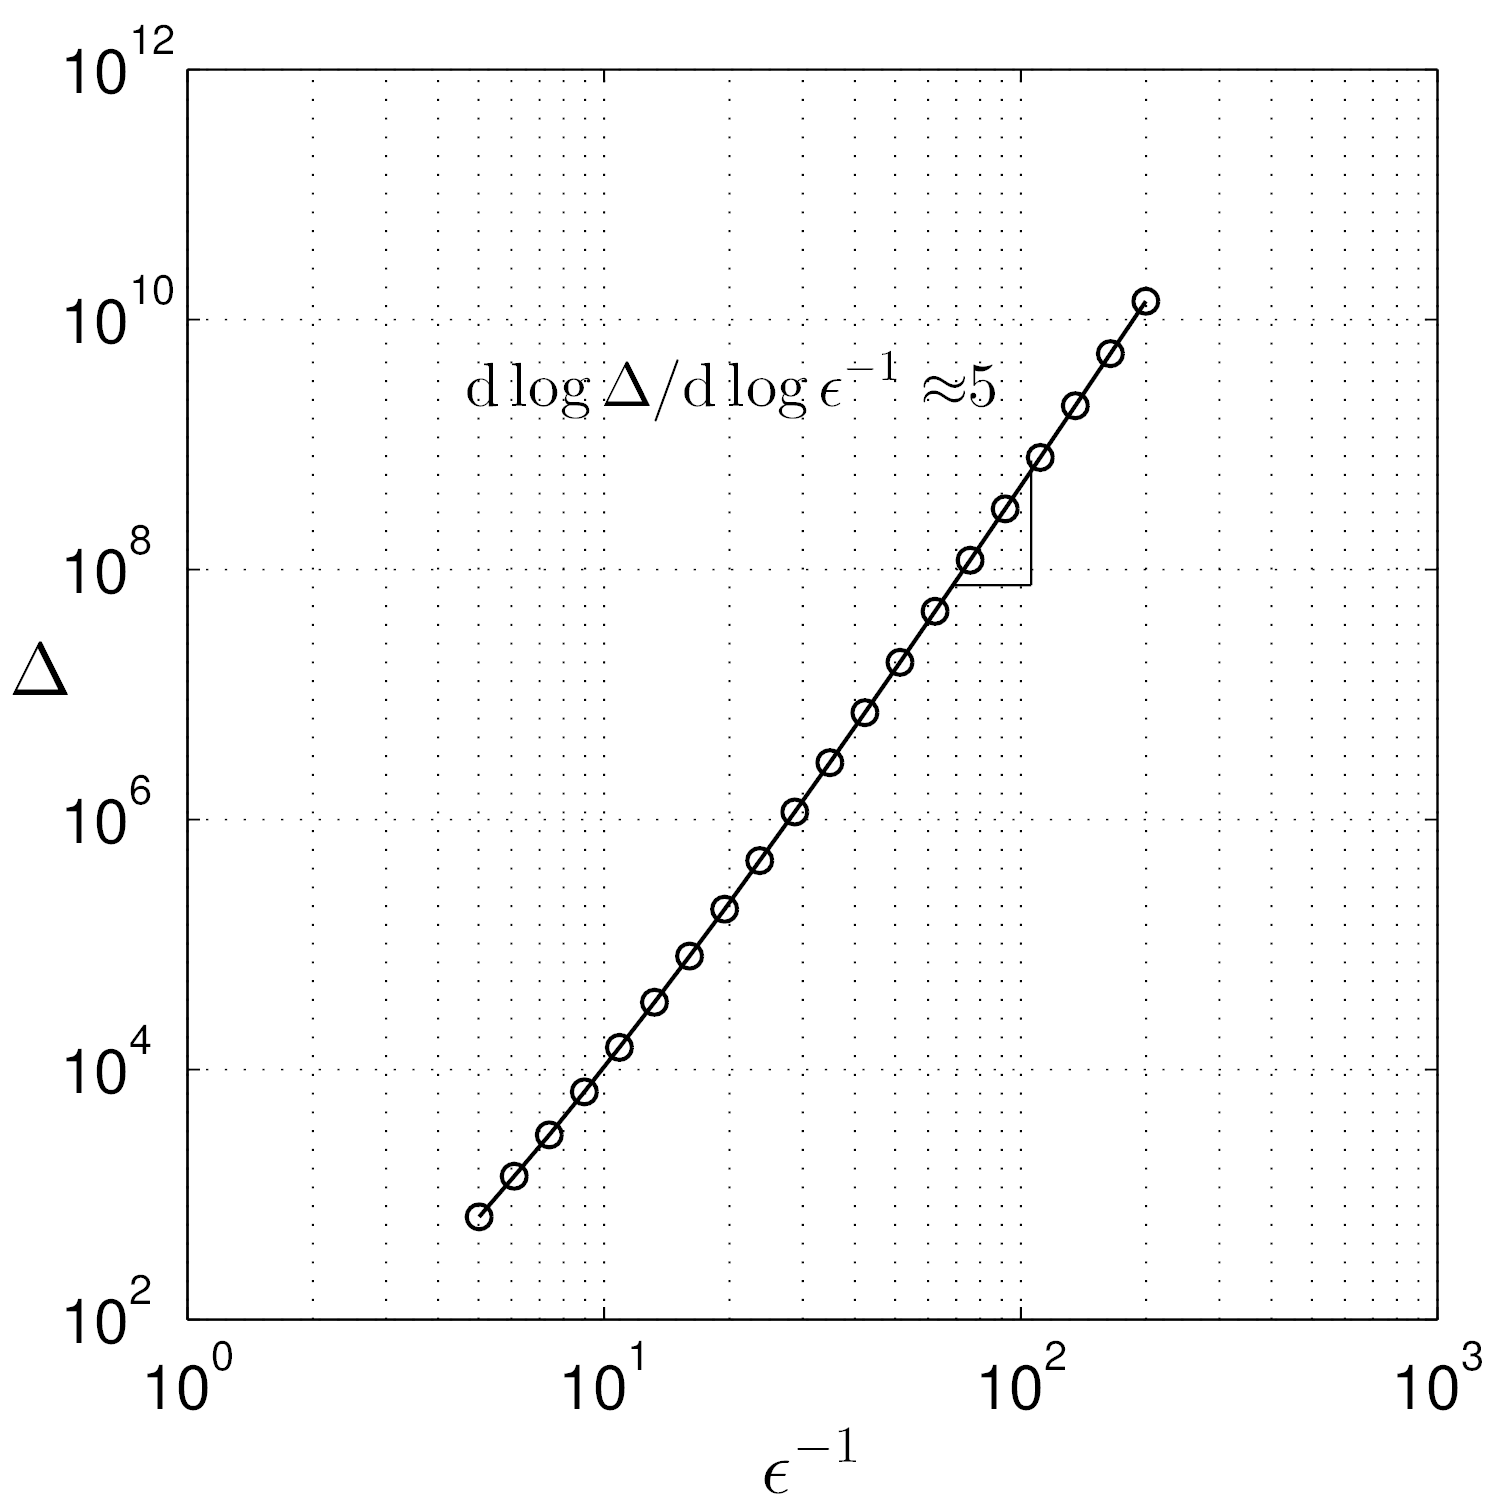
\includegraphics[scale=0.15]{pics/sup_fig6a.png}
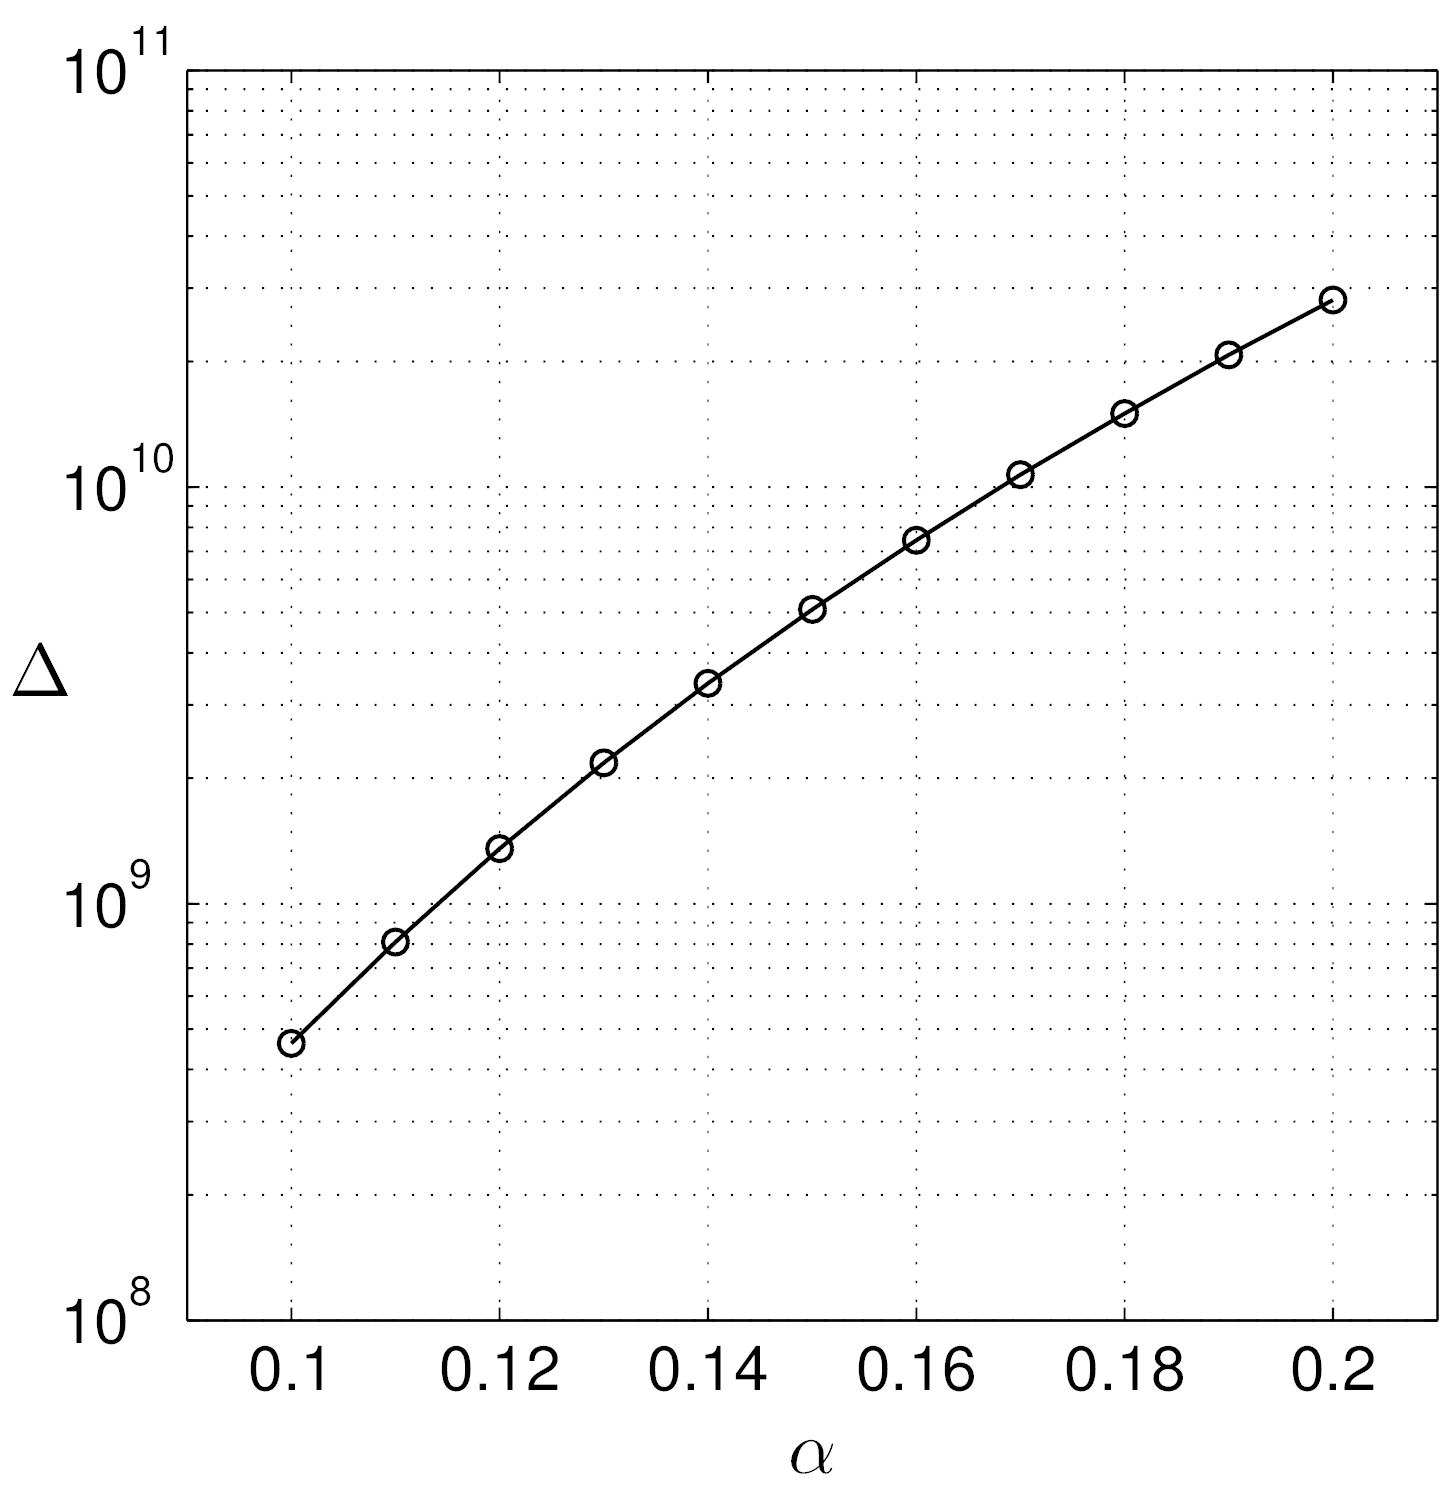
\includegraphics[scale=0.15]{pics/sup_fig6b.png}
\makebox[0.8cm]{}(a)\makebox[8cm]{}(b)
\caption{\normalsize (a) The scaling of minimum $\Delta$ needed to ensure $\|\Sigma_-(z)-H_\text{eff}\|\le\epsilon$ as a function of $\epsilon^{-1}$. Here we choose $\|H_\text{else}\|=0$, $\alpha=0.1$ and $\epsilon$ ranging from $10^{-0.7}$ to $10^{-2.3}$. The values of minimum $\Delta$ are numerically optimized \cite{footnote:num_op}. The slope of the line at large $\epsilon^{-1}$ is $4.97\approx{5}$, which provides evidence that with the assignments of ${\mu}=(\alpha\Delta^4/6)^{1/5}$, the optimal scaling of $\Delta$ is $\Theta(\epsilon^{-5})$. (b) The numerically optimized \cite{footnote:num_op} gap versus the desired coupling $\alpha$ in the target Hamiltonian. Here $\epsilon=0.01$ and $\|H_\text{else}\|=0$.}
\label{fig:ZZZ_fifth_Delta_eps}
\end{figure}

\refsec

\end{comment}

\newpage
\section{Perturbative Direct Gadgets}

Here we do not reduce $k$ by one order at a time (1B1 reduction) or by $\nicefrac{k}{2}$ at a time (SD reduction), but we directly reduce $k$-local terms to 2-local terms.
% Instead of reducing $k$ in a one-by-one (1B1) way, or in a $\nicefrac{k}{2}$-by-$\nicefrac{k}{2}$ way as in sub-division (SD) gadgets, we reduce from $k$-local to 2-local in one step, using $k$  auxiliary qubits for each $k$-local term.

\subsection{PD-JF (Jordan \& Farhi, 2008)}

\summarysec

Express a sum of $k$-local terms as a sum of products of Pauli matrices $s_{ij}$, and define $k$ auxiliary qubits laelled by $a_{ij}$ for each term $i$, and make the transformmation:

\begin{equation}
\sum_i \alpha_i \prod_{j}^k s_{ij} \rightarrow \frac{1}{2} \sum_{i} \sum_{1 \leq j < l \leq k} \left( 1 - z_{a_{ij}} z_{a_{il}} \right) + \epsilon \sum_{i} \left( \alpha_i s_{i1}x_{i1} +  \sum_{j = 2}^k s_{ij}x_{ij} \right) - \sum_{i}\alpha_{i}
\end{equation}

% there is some P_+ operator in JF's Eq. 14
% Above Eq. 8 of JF, tthere's an H_+ which we might need to care about. i.e project the whole of the baove equation onto one subspeace.

\noindent The result is a 2-local Hamiltonian with the same low-lying spectrum to within $\epsilon^{k+1}$ for sufficiently small $\epsilon$.

\notessec
\begin{itemize}
\item $ - \sum_{i}\alpha_{i}$ term not in original paper.
\end{itemize}

\costsec
\begin{itemize}
\item Number of auxiliary qubits is $tk$ for $t$ terms.
\item Unknown requirement for $\epsilon$.
\end{itemize}

\prossec
\begin{itemize}
\item All done in one step, so easier to implement than 1B1 and SD gadgets.
\end{itemize}

%
\conssec
\begin{itemize}
\item Requires 2 more auxiliary qubits per term than 1B1-KKR.
\item Unknown polynomial $f(\lambda)$
\end{itemize}

\examplesec
\begin{align}
3x_{1}y_{2}z_{3} + 5y_{1}z_{2}y_{4} \rightarrow & \frac{1}{2}(6 - z_{a_{11}}z_{a_{12}} - z_{a_{11}}z_{a_{13}} - z_{a_{12}}z_{a_{13}} - z_{a_{21}}z_{a_{22}} - z_{a_{21}}z_{a_{23}} - z_{a_{22}}z_{a_{23}}) \\
& + \epsilon (3x_{1}x_{a_{11}} + y_{2}x_{a_{12}} + z_{3}x_{a_{13}} + 5y_{1}x_{a_{21}} + z_{2}x_{a_{22}} + y_{4}x_{a_{23}}) - 8
\end{align}

\refsec
\begin{itemize}
\item Original paper (Eq. 4-6): \cite{Jordan2008}.
\end{itemize}

\newpage

\subsection{PD-BFBD (Brell, Flammia, Bartlett, Doherty, 2011)}

\summarysec

The 4-body Hamiltonian:

\begin{eqnarray}
H_{\textrm{4-local}} = -\sum_{ij}\left( z_{4i+1,j}z_{4i+2,j}z_{4i+3,j}z_{4i+4,j} + x_{4i+3,j}x_{4i+4,j}x_{4i+6,j}x_{4i+4,j+1}  \right)
\end{eqnarray}

\noindent is transformed into the 2-body Hamiltonian:

\begin{align}
H_{\textrm{2-local}} &= -\sum_{ij} \left( x_{8i+4,j}x_{8i+6,j} + x_{8i+3,j+1}x_{8i+5,j+1} + z_{8i+4,j}z_{8i+3,j+1} + z_{8i+6,j}z_{8i+5,j+1} +  \right.\\
&   + \lambda\left( x_{8i+1,j}x_{8i+3,j+1} + x_{8i+2,j}x_{8i+4,j} + x_{8i+5,j+1}x_{8i+7,j} + x_{8i+6,j}x_{8i+8,j}\right. \\
& + \left.\left.      z_{8i+1,j}z_{8i+3,j+1} + z_{8i+2,j}z_{8i+4,j} + z_{8i+5,j+1}z_{8i+7,j} + z_{8i+6,j}z_{8i+8,j} \right)\right) \
\end{align}

% there is some P_+ operator in JF's Eq. 14
% Above Eq. 8 of JF, tthere's an H_+ which we might need to care about. i.e project the whole of the baove equation onto one subspeace.

\noindent For $\lambda=\mathcal{O}\left(\epsilon^{-5}\right)$, the 2-local Hamiltonian has the same low-lying spectrum as the 4-local Hamiltonian, to within an error of $\epsilon$.

\costsec
\begin{itemize}
\item In total, uses four times the number of qubits of the original Hamiltonian.
\item Unknown requirement for $\lambda$.
\end{itemize}

\prossec
\begin{itemize}
\item All done in one step, so easier to implement than implementing two 1B1 gadgets.
\item Very symmetric
\end{itemize}

%
\conssec
\begin{itemize}
\item Ordinary 1B1 or SD followed by 3$\rightarrow$2 gadgets would require half as many total qubits.
\item Many 2-local terms.
\item Perturbative, as opposed to NR-OY which is similar but does not involve any $\lambda$ parameter.
\item Required value of $\lambda$ for it to work, is presently unknown.
\end{itemize}

%\examplesec

\refsec
\begin{itemize}
\item Original paper (Eq. 3-7): \cite{Brell2011}.
\end{itemize}

\newpage

\subsection{PD-CK (Cao, Kais, 2016)}

\summarysec

 Given a sum of $m$ $k$-local terms, we can define $k$ auxiliary qubits for each $k$-local term and make the following transformation:
\begin{align}
\sum_{i = 1}^{m}a_{i}\prod_{j = 1}^{k}s_{ij} \rightarrow & \sum_{i}\sum_{1 \leq s < t \leq k}\frac{\Delta}{2(k-1)}(1 - z_{a_{is}}z_{a_{it}}) + \sum_{i}\sum_{j}a_{i}^{1/k}s_{ij}x_{ij}
\end{align}

 The result is 2-local and its low-lying spectrum will be the same as the $k$-local Hamiltonian when $\Delta$ is large enough.

\costsec
\begin{itemize}
\item $k$ auxiliary qubits for each $k$-local term, for a total of $km$ auxiliary qubits.
\item $\Delta = O(\epsilon^{-k})$
\end{itemize}

\prossec

\conssec

\examplesec
{\footnotesize
\begin{align}
a_{1}x_{1}x_{2}x_{3} + a_{2}x_{2}y_{4}z_{5} \rightarrow & \frac{\Delta}{4}(3 - z_{a_{11}}z_{a_{12}} - z_{a_{12}}z_{a_{13}} - z_{a_{11}}z_{a_{13}}) + \frac{\Delta}{4}(3 - z_{a_{21}}z_{a_{22}} - z_{a_{22}}z_{a_{23}} - z_{a_{21}}z_{a_{23}}) \\
& + a_{1}^{\nicefrac{1}{3}}(x_{1}x_{a_{11}} + x_{2}x_{a_{12}} + x_{3}x_{a_{13}}) + a_{2}^{\nicefrac{1}{3}}(y_{4}x_{a_{21}} + x_{2}x_{a_{22}} + z_{5}x_{a_{23}})
\end{align}
}

\refsec
\begin{itemize}
\item Original paper (Eq. 4-5, Example on Eq. 44-45): \cite{Cao2017}
\end{itemize}


\newpage
\part{{\normalsize {\underline{Appendix}}}}


%\newpage

\section{Transformations from ternary to binary variables}

\begin{eqnarray}
H_{\textrm{ternary}} = -\lambda (z_1\,z_2+z_1-z_2)
\end{eqnarray}

In this implementation the variable $\frac{1}{2}(z_1+z_2)$ plays the role of $t$, assuming $\lambda$ is large and positive. For instance, when coupled to a binary variable $t\, z_3\rightarrow \frac{1}{2}(z_1+z_2)\,z_3$.

%\section{Notation}
%
%The left Kronecker product by a $2\times2$ identity matrix is implied by Eqs. \eqref{eq:XZ+Z} and \eqref{eq:XX+Z} in the following way for qubit operators $q\in\{z,x\}$, assuming $i<j$:
%Subasi \& Jarzynski (2016)
%
%\begin{align}
%q_{i} & =\mathbf{1}^{\otimes i-1}q\mathbf{1}^{\otimes(N-i+1)}\\
%q_{i}\bar{q}_{j} & =\mathbf{1}^{\otimes i-1}q\mathbf{1}^{\otimes(j-1+i)}\bar{q}\mathbf{1}^{\otimes(N-j+1)}.
%\end{align}
%Thinking in this way, with this notation might take some time to get
%used to, but tens of thousands of people are comfortable thinking
%this way (including any undergraduate student after a 1-semester quantum
%computing course). You can now see that $H$ is a $2^{N}\times2^{N}$
%matrix with elements that are complex numbers. ``Minimizing the Hamiltonian''
%just means finding the eigenvector of this matrix with lowest eigenvalue.
%On a classical computer, the cost of finding this eigenvector is the
%cost of diagonalizing the matrix: $\mathcal{O}(2^{3N})$, but undergraduate
%level quantum mechanics tells us that any physical system's state
%(wavefunction, $\psi_{n}$) is an eigenvector of a Hamiltonian and
%the eigenvalue $E_{n}$ is just the energy associated with being in
%the $n^{{\rm th}}$ energy level:
%\begin{equation}
%H\psi_{n}=E_{n}\psi_{n}.\label{eq:TISE}
%\end{equation}
%Eq. \ref{eq:TISE} is just the time-independent version of the Schroedinger
%equation, which you have at least heard of. The diagonal elements
%are the energies of the $n$ levels and the off-diagonals are associated
%with the propensity for tunnelling from level $n$ to level $m$.
%Any $2^{N}$ level system can be represented by $N$ spin-$\nicefrac{1}{2}$
%particles (\textbf{\uline{qubtis}}), and an example of a spin-$\nicefrac{1}{2}$
%particle is simply an electron. Some of the $N$ electrons will have
%spin up and some will have spin down, hence $2^{N}$ possibilities.
%So instead of $\mathcal{O}(2^{3N})$ operations on a classical computer
%for finding the eigenvector with lowest eigenvalue (and hence doing
%the completely arbitrary computation), we can just (for example) put
%$N$ electrons together %
%\begin{comment}
%such that the $2^{N}$ energy levels have energies $H_{ii}$ and tunelling
%amplitudes $H_{ij}$
%\end{comment}
%with the appropriate $H$ describing their energy, and then cool the
%system down to its ground state. This ground state is one out of $2^{N}$
%possible states , and the configuration of spin up and spin down electrons
%encodes the desired computation.
%
\newpage


\section{Further Examples}

\examplesec \label{subsec:Example_Ramsey_deduc_reduc}
Here we show how deductions can arise naturally from the Ramsey number problem.
Consider $\mathbb{\mathcal{R}}(4,3)$ with $N=4$ nodes.
Consider a Hamiltonian:
\begin{equation}
H = (1-z_{12})(1-z_{13})(1-z_{23})+\ldots+(1-z_{23})(1-z_{24})(1-z_{34})+ z_{12}z_{13}z_{14}z_{23}z_{24}z_{34}.
\end{equation}

\begin{comment}
We should assume there are no 3-independent sets, so we have deductions:
$(1-z_{ij})(1-z_{ik})(1-z_{jk})=0$, for each $i,j,k$.
\end{comment}
See \cite{Okada2015} for full details of how we arrive at this Hamiltonian.

Since we are assuming we have no 3-independent sets, we know that
$(1-z_{12})(1-z_{13})(1-z_{23})=0$, so $z_{12}z_{13}z_{23}=z_{12}z_{13}+z_{12}z_{23}+z_{13}z_{23}-z_{12}-z_{13}-z_{23}+1$.
This will be our deduction.

Using deduc-reduc we can substitute this into our 6-local term to get:
\begin{eqnarray}
H & = & 2(1-z_{12})(1-z_{13})(1-z_{23})+\ldots+(1-z_{23})(1-z_{24})(1-z_{34})+\\
 &  & z_{14}z_{24}z_{34}(z_{12}z_{13}+z_{12}z_{23}+z_{13}z_{23}-z_{12}-z_{13}-z_{23}+1).
\end{eqnarray}

We could repeat this process to remove all 5- and 4-local terms without adding any auxiliary qubits.
Note in this case the error terms added by deduc-reduc already appear in our Hamiltonian.

%3->2-KKR, presented the original way:
%\begin{align}
%\sum_i\prod_j^3 s_{ij} + H_{2-\rm{local}} \rightarrow \frac{1}{24\Delta} \left( \sum_i \left( \sum_j z_{a_{ij}} \right)^2 - \sum_j 1\right) - \frac{1}{6\Delta^{\nicefrac{2}{3}}}\left( \sum_{ij} x_{a_{ij}} \right) - \frac{1}{6\Delta^{\nicefrac{1}{3}}}\left( s_{ij}^2  \right) -\frac{1}{6} H_{\textrm{2-local}}
%\end{align}
%%\sum_i\prod_{j}^k s_{ij} \mapsto \frac{\Delta}{4}\left( 9 - \sum_i \left( \sum_j  z_{a_{ij}} \right)^2 - \sum_j z_{a_{ij}}^2 + \frac{1}{\sqrt[3]{6\Delta}} x_{a_{ij}}  \right).

%\newpage

%\section




\newpage
%\section{$2-$local to $2-$local gadgets}
\section{$2\rightarrow 2$ gadgets}
This review has only focused on $k-$local to $2-$local transformations where $k>2$. There is also a large number of $2-$local to $2-$local transformations in the literature, which are used for various pruposes. Some of these are listed here:

\vspace{10mm}

\begin{itemize}
\item Gadgetization of any $2-$local Hamiltonian into $\{\openone,z,x,zz,xx\}$ or $\{\openone,z,x,zx\}$ \cite{Biamonte2008}. Used for the proof that $xx + zz$ or $xz$ is universal is enough for universal quantum computation. In other words, \textit{any} computation can be transformed into a problem of finding the ground state of a $2-$local Hamiltonian containing terms from $\{\openone,z,x,zz,xx\}$ or from $\{\openone,z,x,zx\}$ with real coefficients, and the ground state can be found by adiabatic quantum computing with only polynomial time and space overhead over the best alternative algorithm for the problem.

\item Transformation of any $2-$local Hamiltonian into $\{\openone,z,x,zz,xx+yy\}$, without any perturbative gadgets, and only requiring the qubits to be connected in an almost 2D lattice \cite{Lloyd2016}.


\item "Cross gadget", "fork gadget", and "triangle gadget" described in \cite{Oliveira2008}.
\item Gadgetizeation of a $2-$local Hamiltonian with very strong couplings, into a $2-$local Hamiltonian with strengths in $\mathcal{O}\left( \nicefrac{1}{\textrm{poly}\left( \epsilon^{-1},n\right)}  \right)$, and $\textrm{poly}\left( \epsilon^{-1},n  \right)$ auxiliary qubits and $\textrm{poly}\left( \epsilon^{-1},n  \right)$ new quadratic terms. \cite{Cao2015a}.
\item $yy$ creation gadget: Simulation of $yy$ terms  using $\{\openone,z,x,zz,xx\}$, with coupling strength restriction defined according to $\Delta = \Theta\left(\epsilon^{-4}\right)$ \cite{Cao2015}. % they do not even say they need \openone, but maybe they are ignoring it due to causing a constant shift.
\end{itemize}

\subsection{Minor-embedding quadratic functions for different graphs}
\begin{itemize}
\item Minor-embedding general problems for the Chimera  \cite{Neven2009} graph \cite{vchoi08,Choi2011a}.
\item Minor-embedding quadratization gadgets for the Pegasus  \cite{Dattani2019b} graph \cite{Dattani2019c}.
\end{itemize}



\newpage




\section{Further References}
\begin{itemize}
\item Gadgets for pseudo-Boolean optimization problems, with reduced precision requirements: \cite{Babbush2013}.
\item Formalization of pseudo-Boolean gadgets in quantum language. \cite{Biamonte2008a}.
\item By adding more couplers and more auxiliary qubits, we can bring the error down arbitrarily low:  \cite{Cao2015a}.
\item More toric code gadgets: \cite{Brell2014}.
\item Parity adiabatic quantum computing (LHZ lattice): \cite{Lechner2015}.
\item Extensions of the LHZ scheme: \cite{Rocchetto2016}.
\item Minimizing $k$-local discrete functions with the help of continuous variable calculus \cite{Shen2017a}.
\item ORI graph which attempts to give optimal quadratizations \cite{Gallagher2011}.
\item Survey on pseudo-Boolean optimization \cite{Boros2002}.
\item Linearization of equations before they are squared \cite{Schaller2010}, and its application to factoring numbers \cite{Xu2012}.
\item Mentioned in \cite{Ali2008} as an early application of quadratization: \cite{Cunningham1985}.
\item Characterizaton of NTRs for cubics: \cite{Crama2014a}.
\item Relation between cones of nonnegative quadratic pseudo-Boolean functions and the Boolean quadric polytope \cite{BorosLari2014}.
\item Relation between cones of nonnegative quadratic pseudo-Boolean functions and the Boolean quadric polytope \cite{BorosLari2014}.
\item Effective non-Hermitian Hamiltonian with 3-body interactions which helps to calcualte electronic structure energies closer to the complete basis set limit \cite{Cohen2019}.
\item Hubbard-Stratonovich transformation \cite{Stratonovich1957,Hubbard1959} is used to derive Eq. 10a, 10b, and 10c of \cite{Hirsch1983}, in which the exponential of a quadratic equals the trace/integral of an exponential of something linear. In the case where the number operator is written as a product of two operators, this means a 4-body operator in the exponent becomes a 2-body operator in the exponent.
%\item Verma-Lewis paper
%\item Aritanan Gruber's thesis on quadratization \cite{}.
% 25:30 of Lechner's 2016 AQC talk mentions another paper that can do 4-local to 2-local with 1 auxiliary using 5 connections (better than Ishikawa which requires 15?).
% LHZ can do k-local to 4-local (?) with maybe (N choose k) auxiliaries. (N choose 2) for 2-local, (N choose 3) for 3-local, etc. look into
% Lechner's talk says that Rocchetto's scheme can add k-locals to LHZ lattice by sacrificing not being able to do all-2-all
% Gruber's review paper with Boros
% The other things in the LyX file
% Gruber's suggested papers (the Oxford guys, for example), and a book he mentioned which I haven't looked at yet.
% LZL: k-local to 3-local
% Toby's k-local to 3-local
% Richard's technique for using most methods on MULTIPLE terms
% Ocko-Yoshida's original scheme, quantum double scheme, and triangular lattice
% Brell's 2014 paper.
%PTR inspired by NTR-KZFD on bit flipped variables is given. What about with NTR-ABCB?
\end{itemize}

\newpage
\section{Circuits that effectively implement degree-$k$ terms for superconducting qubits}
\begin{itemize}
\item Presentation by Northrop Grumman about a $zzz$ coupler \cite{Strand2017} and associated patent \cite{Ferguson2017,Ferguson2018}.
\item Presentaiton that included discussion about engineering multi-qubit interactions \cite{Kerman2018}, presentation by the same lab about the design and experimental demonstration of a $zzzz$ coupling \cite{Menke2019}, and associated patent \cite{Kerman2018a,Kerman2019,Kerman2019a}.
\item Design of an effective $zzzz$ coupling without any auxiliary logical qubits \cite{Schondorf2018}.
\item Design of a tunable $zzz$ coupling with 2 auxiliary qubits in which all $zz$ couplings are cancelled, and its experimental demonstration \cite{Melanson2019}.
\end{itemize}

\newpage

% add NMR papers that implement multi-body physics.

\section{Contributors}

\subsection*{Richard Tanburn}
\begin{itemize}
\item Richard was the original creator and maintaner of the Git repository.
\item Richard created the Tex commands used throughout the document, and contributed majorly to the overall layout.
\item Richard wrote the original versions of the following sections: (1) Deduc-Reduc, (2) ELC Reduction, (3) Groebner Bases, (4) Split Reduction, (5) NTR-KZFD, (6) NTR-GBP, (7) PTR, (8) PTR-Ishikawa, (9) PTR-KZ, (10) PTR-GBP, (11) Bit flipping, (12) RBS, and (13) FGBZ.
\item Richard also wrote the "Further Example" of Deduc-Reduc in the Appendix.
% need to check some of these, for example, was NTR-KZFD there in the original version?, which Boros 2018 ones did he actually add? I know there was one  I told him to add from Wikipedia and he didn't add much so I had to do things.
\end{itemize}

\subsection*{Nicholas Chancellor}
\begin{itemize}
\item Nick made contributions to the following sections: (1) RMS (in terms of z), (2) PTR-RBL-(3$\rightarrow$2), (3) PTR-RBL-(4$\rightarrow$2), (4) SBM, (5) Flag based SAT Mapping, and to the qutrit $\rightarrow$ qubit transformation (6).
\end{itemize}

\subsection*{Szilard Szalay}
\begin{itemize}
\item Szilard re-derived Nike's transformations for the sections: (1) SFR-BCR-1, (2) SFR-BCR-2, (3) SFR-BCR-3, and (4) SFR-BCR-4 from the notation of the original paper, into the format consistent with the rest of the book. In doing so he corrected errors in Nike's work and also fixed them in the main document.
\end{itemize}

\subsection*{Ka Wa Yip}
\begin{itemize}
\item Ka Wa Yip the original verison of a section which was later converted by Nike into the following two sections: (1) NTR-YXKK, and (2) PTR-YXKK.
\end{itemize}

\subsection*{Yudong Cao}
\begin{itemize}
\item Yudong wrote the first version of the following section: (1) PSD-CN.
\end{itemize}

\subsection*{Daniel Nagaj}
\begin{itemize}
\item Daniel provided a .tex document to Nike in May 2018 which helped Nike to write the following sections: (1) NP-Nagaj-1, (2) NP-Nagaj-2. The document that Daniel provided made it easier for Nike to write these sections than the original papers.
\end{itemize}

\subsection*{Aritanan Gruber}
\begin{itemize}
\item Aritanan informed us in August 2015 of what we ended up making the following sections: (1) PTR-Ishikawa. % and much more, look through the emails.
\end{itemize}

\subsection*{Charles Herrmann}
\begin{itemize}
\item Charles informed us in May 2018 of the papers which contained results which became the following sections: (1) PTR-BCR-1,  (2) PTR-BCR-2, (3) PTR-BCR-3, (4) PTR-BCR-4, (5) SFR-BCR-1, (6) SFR-BCR-2, (7) SFR-BCR-3, (8) SFR-BCR-4, (9) SFR-BCR-5, (10) SFR-BCR-6. % need to read emails to get the other things.
\end{itemize}

\subsection*{Elisabeth Rodriguez-Heck}
\begin{itemize}
\item Elisabeth provided us with a 2-page PDF document with valuable comments on the entire Book.
\item Elisabeth also pointed us to what became the following section: (1) ABCG Reduction.
\end{itemize}

\subsection*{Hou Tin Chau}
\begin{itemize}
\item Tin made the examples for the following sections: SFR-BCR-1,2,3,4.
\item Tin fixed a typo in the alternative forms of the following sections: SFR-BCR-3,4.
\end{itemize}

\subsection*{Andreas Soteriou}
\begin{itemize}
\item Andreas found typos on the opening page in the arXiv version which surprisingly no one else found (or pointed out), and he diligently fixed them.
\item Andreas created the example involving $x$,$y$, and $z$ presented on the opening page in the September 2019 version (I plan to have this example further improved at a later time).
\item Andreas added the minimum and maximum coefficient ranges into the cost section for PTR-BCR-4.
\end{itemize}

\subsection*{Jacob Biamonte}
\begin{itemize}
\item Jacob made valuable edits during a proof-reading of the book.
\end{itemize}



\newpage

\section*{Acknowledgments}
\begin{itemize} % check when Toby helped us with the bit-flipping stuff
\item It is with immense pleasure that we thank Emile Okada of Cambridge University, who during his first year of udnergraduate study, worked with Nike Dattani and Richard Tanburn on quadratization of pseudo-boolean functions for quantum annealing, and in the first half of 2015 played a role in the development of the Deduc-Reduc and Split-Reduc and Groebner bases methods presented in this review.
\item We thank Gernot Schaller of University of Berlin, who in December 2014 provided Nike Dattani with insights into his quadratization methods mentioned in this review paper, as well as for sharnig his Mathematica code which could be used to generate such quadratization formulas and others.
\item We thank Mohammad Amin of D-Wave for pointing Nike Dattani to the paper \cite{Bian2013} on determining Ramsey numbers on the D-Wave device, which contained what we call in this review "Reduction by substitution", later found through Ishikawa's paper to be from the much older 1970s paper by Rozenberg.
\item We thank Catherine McGeoch of Amherst University and D-Wave, for helpful discussions with Nike Dattani in December 2014 about how to map quadratic pseudo-Boolean optimization problems onto the chimera graph of the D-Wave hardware and for pointing us to the important references of Vicky Choi. While chimerization is very different from quadratization, understanding that roughly $n^2$ variables would be needed to map a quadratic function of $n$ variables, helped Nike Dattani and Richard Tanburn to appreciate how impotrant it is to be able to quadratize with as few variables as possible, and having this in mind throughout our studies helped inspire us in our goals towards "optimal quadratization".
\item We thank Aritanan Gruber and Endre Boros of Rutgers University, who in August 2015 shared with Nike Dattani and Richard Tanburn some of their wisdom about sub-modularity, and Aritanan Gruber for pointing us to the then very recent paper of Hiroshi Ishikawa on what we call in this review "ELC reductions", which was also a valuable paper due to the references in it. We also thank him for helping us in our quest to determine whether or not "deduc-reduc" was a re-discovery by Richard, Emile, and Nike, or perhaps a novel quadratization scheme.
\item We thank Toby Cathcart-Burn of Oxford University, who during the third year of undergraduate study, worked with Nike Dattani and Richard Tanburn and in Autumn 2015 and Winter 2016 helped us gain insights about the application of deduc-reduc and bit flipping to the problem of determining Ramsey numbers via discrete optimization, and for insights into the trade-offs between Ishikawa's symmetric reduction and reduction by substitution.
\item  We thank Hiroshi Ishikawa of Waseda University, who Nike Dattani had the memorable opportunity to visit in November 2015, and through discussions about the computer vision problem and neural network problem (two examples of real-world discrete optimization problems that benefit from quadratization), provided insights about the role of quadratization for calculations on classical computers. In particular, solving the computer vision problem in which he had experience solving on classical computers, was very different from the integer factoring problem and Ramsey number problem which we had been attempting to quadratize for D-Wave and NMR devices. He taught us that far more total (original plus auxiliary) variables can be tolerated on classical computers than on D-Wave machines or NMR systems, and approximate solutions to the optimization problems are acceptable (unlike for the factorization and Ramsey number problems in which we were interested). This gave us more insight into what trade-offs one might wish to prioritize when quadratizing optially. We also thank him for helping us in our quest to determine whether or not "deduc-reduc" was a re-discovery by Richard, Emile, and Nike, or perhaps a novel quadratization scheme.
\item We thank Salil Bedkihal for informing Nike of the paper by Hirsch which uses the Hubbard-Stratonovich transformation, now mentioned in the "Further References" section.
\item Last but indubitably not least, we thank Jacob Biamonte of Skolkovo Institute of Technology, who Nike Dattani enjoyed visiting in Hangzhou in January 2017 and meeting at Harvard University in April 2018. Jacob provided us plenty of insights about perturbative gadgets, made valuable comments on early versions of our manuscript, and has been a major supporter of this review paper since the idea was presented to him in December 2016. At many points during the preparation of this review, we had prioritized other commitments and put preparation of this review aside. Jake's frequent encouragement was often what got us working on this review again. Without him, we are not certain this paper would have been completed by this time (or ever!).
%Mike Mosca for Grubner Bases suggestion.
%Bill McGreedy for finding bug in split-redc code.
%Ojas Metha
%Peng, Du, Li, Ke, Chen?  Osaka City University
%Alex McCaskey, since in recent times I've been working hard on this to give him something easy to work with ???
% Courtney Brell from the Toric codes.
% Terhal
% Ocko
% Nagaj
% Charles, Zabih
% More Ishikawa
% More Gruber?

% Combining gadgets together. CBBK talks about parallel subdivision, and BDLT has a section on "combining the gadgets together" mainly useful for looking at the error analysis.

\end{itemize}











\newpage
%\bibliographystyle{apsrev4-1}
\bibliography{k-local-quadratization}

\end{document}

% More ideas.
%---------- Forwarded message ----------
%From: Nike Dattani <dattani.nike@gmail.com>
%Date: 20 October 2015 at 18:02
%Subject: Re: Quantum Computing Project
%To: Toby Cathcart Burn <toby.cathcartburn@merton.ox.ac.uk>
%
%
%Dear Toby,
%
%I can see some easy ways of doing better than M-3 or M-4 extra qubits. Simply pairing variables halves the number of extra qubits required if you use Ishikawa's method, while giving a few quartics;
%
%If by "simply pairing" you mean x1x2x3x4 -> y1y2, where y1=x1x2 and y2=x3x4, I can see how it halves the number of extra qubits, and how it introduces the quartic term a*y1y2. I can also see that the cubic term introduced has negative coefficient, so can be quadratized with only 1 qubit.
%
%...
%
%and similar pairing can be used to modify the penalty function given in the appendix to replace a cubic(quartic) with a single variable using only cubic(quartic) terms.

%%%%%%%%%%%%% MUST ADD CITATION TO KEMPE REGEV KITAEV !!!!!!11
